% !TeX encoding = UTF-8
% !TeX program = xelatex
% !TeX spellcheck = en_US

\documentclass[degree=master]{thuthesis}
  % 学位 degree:
  %   doctor | master | bachelor | postdoc
  % 学位类型 degree-type:
  %   academic(默认)| professional
  % 语言 language
  %   chinese(默认)| english
  % 字体库 fontset
  %   windows | mac | fandol | ubuntu
  % 建议终版使用 Windows 平台的字体编译


% 论文基本配置,加载宏包等全局配置
% !TeX root = ./thuthesis-example.tex

% 论文基本信息配置

\thusetup{
  %******************************
  % 注意:
  %   1. 配置里面不要出现空行
  %   2. 不需要的配置信息可以删除
  %   3. 建议先阅读文档中所有关于选项的说明
  %******************************
  %
  % 输出格式
  %   选择打印版(print)或用于提交的电子版(electronic),前者会插入空白页以便直接双面打印
  %
  output = print,
  %
  % 标题
  %   可使用“\\”命令手动控制换行
  %
  title  = {基于最优控制理论的触摸运动模型},
  title* = {Modeling, Sensing and Understanding Pervasive Touch Input},
  %
  % 学位
  %   1. 学术型
  %      - 中文
  %        需注明所属的学科门类,例如:
  %        哲学、经济学、法学、教育学、文学、历史学、理学、工学、农学、医学、
  %        军事学、管理学、艺术学
  %      - 英文
  %        博士:Doctor of Philosophy
  %        硕士:
  %          哲学、文学、历史学、法学、教育学、艺术学门类,公共管理学科
  %          填写“Master of Arts“,其它填写“Master of Science”
  %   2. 专业型
  %      直接填写专业学位的名称,例如:
  %      教育博士、工程硕士等
  %      Doctor of Education, Master of Engineering
  %   3. 本科生不需要填写
  %
  degree-name  = {工学博士},
  degree-name* = {Doctor of Philosophy},
  %
  % 培养单位
  %   填写所属院系的全名
  %
  department = {计算机科学与技术系},
  %
  % 学科
  %   1. 学术型学位
  %      获得一级学科授权的学科填写一级学科名称,其他填写二级学科名称
  %   2. 工程硕士
  %      工程领域名称
  %   3. 其他专业型学位
  %      不填写此项
  %   4. 本科生填写专业名称,第二学位论文需标注“(第二学位)”
  %
  discipline  = {计算机科学与技术},
  discipline* = {Computer Science and Technology},
  %
  % 姓名
  %
  author  = {古裔正},
  author* = {Gu Yizheng},
  %
  % 指导教师
  %   中文姓名和职称之间以英文逗号“,”分开,下同
  %
  supervisor  = {史元春, 教授},
  supervisor* = {Professor Shi Yuanchun},
  %
  % 副指导教师
  %
  associate-supervisor  = {喻纯, 副教授},
  associate-supervisor* = {Associate Professor Yu Chun},
  %
  % 联合指导教师
  %
  % co-supervisor  = {某某某, 教授},
  % co-supervisor* = {Professor Mou Moumou},
  %
  % 日期
  %   使用 ISO 格式;默认为当前时间
  %
  % date = {2019-07-07},
  %
  % 是否在中文封面后的空白页生成书脊(默认 false)
  %
  include-spine = false,
  %
  % 密级和年限
  %   秘密, 机密, 绝密
  %
  % secret-level = {秘密},
  % secret-year  = {10},
  %
  % 博士后专有部分
  %
  % clc                = {分类号},
  % udc                = {UDC},
  % id                 = {编号},
  % discipline-level-1 = {计算机科学与技术},  % 流动站(一级学科)名称
  % discipline-level-2 = {系统结构},          % 专业(二级学科)名称
  % start-date         = {2011-07-01},        % 研究工作起始时间
}

% 载入所需的宏包

% 定理类环境宏包
\usepackage{amsthm}
% 也可以使用 ntheorem
% \usepackage[amsmath,thmmarks,hyperref]{ntheorem}

\thusetup{
  %
  % 数学字体
  % math-style = GB,  % GB | ISO | TeX
  math-font  = xits,  % sitx | xits | libertinus
}

% 可以使用 nomencl 生成符号和缩略语说明
% \usepackage{nomencl}
% \makenomenclature

% 表格加脚注
\usepackage{threeparttable}

% 表格中支持跨行
\usepackage{multirow}

% 固定宽度的表格。
% \usepackage{tabularx}

% 跨页表格
\usepackage{longtable}

% 算法
\usepackage{algorithm}
\usepackage{algorithmic}

% 量和单位
\usepackage{siunitx}

% 参考文献使用 BibTeX + natbib 宏包
% 顺序编码制
\usepackage[sort]{natbib}
\bibliographystyle{thuthesis-numeric}

% 著者-出版年制
% \usepackage{natbib}
% \bibliographystyle{thuthesis-author-year}

% 本科生参考文献的著录格式
% \usepackage[sort]{natbib}
% \bibliographystyle{thuthesis-bachelor}

% 参考文献使用 BibLaTeX 宏包
% \usepackage[backend=biber,style=thuthesis-numeric]{biblatex}
% \usepackage[backend=biber,style=thuthesis-author-year]{biblatex}
% \usepackage[backend=biber,style=apa]{biblatex}
% \usepackage[backend=biber,style=mla-new]{biblatex}
% 声明 BibLaTeX 的数据库
% \addbibresource{ref/refs.bib}

% 定义所有的图片文件在 figures 子目录下
\graphicspath{{figures/}}

% 数学命令
\makeatletter
\newcommand\dif{%  % 微分符号
  \mathop{}\!%
  \ifthu@math@style@TeX
    d%
  \else
    \mathrm{d}%
  \fi
}
\makeatother

% hyperref 宏包在最后调用
\usepackage{hyperref}



\begin{document}

% 封面
\maketitle

% 学位论文指导小组、公开评阅人和答辩委员会名单
% !TeX root = ../thuthesis-example.tex

\begin{committee}[name={学位论文指导小组、公开评阅人和答辩委员会名单}]

  \newcolumntype{C}[1]{@{}>{\centering\arraybackslash}p{#1}}

  \section*{指导小组名单}

  \begin{center}
    \begin{tabular}{C{3cm}C{3cm}C{9cm}@{}}
      李XX & 教授     & 清华大学 \\
      王XX & 副教授   & 清华大学 \\
      张XX & 助理教授 & 清华大学 \\
    \end{tabular}
  \end{center}


  \section*{公开评阅人名单}

  \begin{center}
    \begin{tabular}{C{3cm}C{3cm}C{9cm}@{}}
      刘XX & 教授   & 清华大学                    \\
      陈XX & 副教授 & XXXX大学                    \\
      杨XX & 研究员 & 中国XXXX科学院XXXXXXX研究所 \\
    \end{tabular}
  \end{center}


  \section*{答辩委员会名单}

  \begin{center}
    \begin{tabular}{C{2.75cm}C{2.98cm}C{4.63cm}C{4.63cm}@{}}
      主席 & 赵XX                  & 教授                    & 清华大学       \\
      委员 & 刘XX                  & 教授                    & 清华大学       \\
          & \multirow{2}{*}{杨XX} & \multirow{2}{*}{研究员} & 中国XXXX科学院 \\
          &                       &                         & XXXXXXX研究所  \\
          & 黄XX                  & 教授                    & XXXX大学       \\
          & 周XX                  & 副教授                  & XXXX大学       \\
      秘书 & 吴XX                  & 助理研究员              & 清华大学       \\
    \end{tabular}
  \end{center}

\end{committee}



% 也可以导入 Word 版转的 PDF 文件
% \begin{committee}[file=figures/committee.pdf]
% \end{committee}


% 使用授权的说明
\copyrightpage
% 将签字扫描后授权文件 scan-copyright.pdf 替换原始页面
% \copyrightpage[file=scan-copyright.pdf]

\frontmatter
% !TeX root = ../thuthesis-example.tex

% 中英文摘要和关键字

\begin{abstract}

% [V1] 触摸输入是自然人机交互的重要组成部分,在过去和当下,人通过触屏设备向计算机输入信息。随着AR头盔、智能手表等可穿戴设备的发展,交互向着普适计算的方向发展,在未来,人能在任何时间地点、以任何形式进行信息的获取和处理。在此背景下,本文提出\textbf{普适触摸输入}的概念:\textit{人能在任何表面,如桌面、墙面和手掌上通过触摸向计算机输入信息;触摸输入感知摆脱对触屏的依赖,转而利用可穿戴设备等普适计算单元识别}。本文研究普适触摸输入的感知技术,有两大难点:(1)难点一是判断人是否触摸了表面。人对触摸交互的敏感程度高,在判别准确率、延迟和定位精度这三方面给触摸感知提出了高要求。在普适触摸模态下,不可能在任意表面上加装传感器,而是利用普适计算单元识别,感知难度大大提升。(2)难点二是判断触摸是否表达交互意图。当人能在任意表面触摸输入,表面就同时具有物理属性和数字属性,人触摸表面具有二义性,既可能表达数字交互意图,也可能是利用表面的物理属性。因此,系统需要判断触摸是否表达交互意图,防止误触。本文基于普适触摸输入的行为模型,提出了多信道融合的触摸感知技术,准确、快速感知普适触摸,同时利用连续触摸的时空相关性表征人的触摸行为,有效辨识触摸是否表达交互意图。具体研究贡献包括:(1)提出了触摸的多信道行为模型:本文研究了触摸的行为模型,从视觉、听觉、震动等多个信道总结了触摸瞬间的客观物理现象规律。(2)提出了多信道融合的触摸感知技术:针对触摸感知在判别、延迟和定位这三方面的性能需求,本文结合各信道上突出的信号特征,实现了高性能的普适触摸输入感知技术,判别准确率大于98.5\%,延迟小于10毫秒,定位误差小于1厘米。(3)提出了多信道融合的触摸意图推理技术:在普适触摸输入模态下,系统需要鉴别触摸是否表达数字意图,防止误触。本文提出利用连续触摸的时空相关性表征触摸行为的方法,实现了准确的普适触摸输入意图推理技术。在最复杂的触摸输入任务——文本输入实验的验证下,该技术的防误触能力达到98.9\%。

%探索触摸前后多维度行为数据的时空相关性特征,本文针对多种触摸交互任务(目标选择、文本输入)提高交互效率,本文改进了触摸的感知和意图推理技术,从而改善用户体验。触摸的多信道融合模型为触摸的感知和交互技术提供了有效的计算理论基础,在此融合的模型的支持下,本文从三个方向改进了触摸感知和交互技术,具体贡献如下:

%如何建模和利用触摸的多信道特征,是触摸交互的重要研究问题——多信道融合技术将在广度和深度上改进触摸交互技术:(1)广度上,基于多信道融合的穿戴式传感技术将支持普通表面上的触摸感知,赋能桌面、墙面上的触摸交互,使触摸交互摆脱对触屏的依赖;(2)深度上,基于多信道融合的意图推理技术将准确区分有意触摸输入和无意触碰。本文提出触摸的多信道融合模型,探索触摸在视觉、声音、震动和压力等维度上的时空相关性特征,针对多种触摸交互任务(目标选择、文本输入)提高交互效率,改进触摸的感知和意图推理技术,从而改善用户体验。具体研究贡献包括:

%(1)提出了触摸的多信道融合模型:针对相关工作在触摸的视觉、声音、震动、压力等信道上存在空缺的研究现状,本文提出了触摸的多信道融合模型,为触摸交互技术的改进提供了计算理论基础。该模型是在广度和深度上提升触摸交互能力的利器,以下两条贡献均为其应用实例。

【题目】基于最优控制理论的触摸运动模型

触摸交互是重要的人机交互方式,是人控制手指触摸交互表面,通过点击、长按、滑动等手势向计算机输入信息的方式。尽管触摸交互的主要载体触摸屏已问世数十年,触摸交互仍存在三点不足:(1)普适性:触摸交互被限制于有源表面上,不满足普适计算中人随时随地与计算机交互的需求;(2)响应性:人对触摸交互响应性的感官需求极高,能察觉到低至10毫秒的延迟,而常用触摸屏的延迟为50毫秒,不能提供最佳用户体验;(3)意图性:人机交互朝着自然动作输入的方向发展,而自然触摸交互中人的有意触摸和无意触碰混杂,误触更频繁。为克服上述不足,设计无源、低延迟、精准的触摸交互技术,本文提出了基于最优控制理论的触摸运动模型,揭示触摸前后极短时间内手指的运动规律。该模型为基于运动传感(包括位移、速度和加速度)的触摸交互技术提供了计算理论基础。基于模型,本文针对多种触摸交互任务(目标选择、文本输入),优化触摸感知和防误触技术,提升交互效率和用户体验。具体贡献如下:

(1)提出了基于最佳控制理论的触摸运动模型,包含数学模型(描述触摸运动的数学方程)和计算模型(利用位移、速度、加速度传感信号拟合触摸运动方程的计算方法)。本文详细描述了模型的表达、提出过程和推导过程,通过实验验证了模型的有效性,最后讨论了模型在普适性、响应性和意图性三方面对触摸交互技术的指导意义。

(2)提出了基于运动传感指环的低延迟触摸感知技术:基于指环的触摸感知技术使用户能在无源表面(如桌面、墙面)上触摸输入[xx],具有较强的普适性。先前工作利用阈值方法感知触摸[xx],延迟高达200毫秒,准确率仅为85\%[xx]。本文基于触摸运动模型,提出了低延迟的基于指环的触摸感知技术,延迟低于10毫秒,准确率超过99\%。低延迟是技术的关键,由于用户无法在触摸交互中察觉到低于10毫秒的延迟,该技术理论上提供了最佳用户体验。

(3)提出了面向连续触摸输入的防误触技术:文本输入是最复杂的连续触摸输入任务,针对触摸屏十指文本输入中用户频繁误触的问题,本文提出基于触摸运动模型的防误触技术。本文通过文本输入任务评测防误触技术的性能,防误触技术的准确率达到99\%,且允许用户在打字时将非交互手指休息在触摸屏上(而不会引发误触),将打字速率提升20\%。

% (4)触摸运动模型为触摸交互技术提供了计算理论基础,对触摸交互技术具有指导性意义。例如,众多研究者利用视觉方法识别触摸,却受困于视线遮挡问题[xx]。我们的模型指出,触摸瞬间手指发生毫秒级的瞬停现象,因此触摸感知不一定要观察到接触本身,而可以检测手指是否瞬停,从而绕过遮挡问题。

  % 关键词用“英文逗号”分隔,输出时会自动处理为正确的分隔符
  \thusetup{
    keywords = {触摸交互, 感知技术, 意图识别},
  }
\end{abstract}

\begin{abstract*}
  An abstract of a dissertation is a summary and extraction of research work and contributions.
  Included in an abstract should be description of research topic and research objective, brief introduction to methodology and research process, and summary of conclusion and contributions of the research.
  An abstract should be characterized by independence and clarity and carry identical information with the dissertation.
  It should be such that the general idea and major contributions of the dissertation are conveyed without reading the dissertation.

  An abstract should be concise and to the point.
  It is a misunderstanding to make an abstract an outline of the dissertation and words “the first chapter”, “the second chapter” and the like should be avoided in the abstract.

  Keywords are terms used in a dissertation for indexing, reflecting core information of the dissertation.
  An abstract may contain a maximum of 5 keywords, with semi-colons used in between to separate one another.

  % Use comma as separator when inputting
  \thusetup{
    keywords* = {keyword 1, keyword 2, keyword 3, keyword 4, keyword 5},
  }
\end{abstract*}


% 目录
\tableofcontents

% 插图和附表清单
% 本科生的插图索引和表格索引需要移至正文之后、参考文献前
\listoffiguresandtables  % 插图和附表清单
% \listoffigures           % 插图清单
% \listoftables            % 附表清单

% 符号对照表
% !TeX root = ../thuthesis-example.tex

\begin{denotation}[3cm]
  \item[PI] 聚酰亚胺
  \item[MPI] 聚酰亚胺模型化合物,N-苯基邻苯酰亚胺
  \item[PBI] 聚苯并咪唑
  \item[MPBI] 聚苯并咪唑模型化合物,N-苯基苯并咪唑
  \item[PY] 聚吡咙
  \item[PMDA-BDA] 均苯四酸二酐与联苯四胺合成的聚吡咙薄膜
  \item[MPY] 聚吡咙模型化合物
  \item[As-PPT] 聚苯基不对称三嗪
  \item[MAsPPT] 聚苯基不对称三嗪单模型化合物,3,5,6-三苯基-1,2,4-三嗪
  \item[DMAsPPT] 聚苯基不对称三嗪双模型化合物(水解实验模型化合物)
  \item[S-PPT] 聚苯基对称三嗪
  \item[MSPPT] 聚苯基对称三嗪模型化合物,2,4,6-三苯基-1,3,5-三嗪
  \item[PPQ] 聚苯基喹噁啉
  \item[MPPQ] 聚苯基喹噁啉模型化合物,3,4-二苯基苯并二嗪
  \item[HMPI] 聚酰亚胺模型化合物的质子化产物
  \item[HMPY] 聚吡咙模型化合物的质子化产物
  \item[HMPBI] 聚苯并咪唑模型化合物的质子化产物
  \item[HMAsPPT] 聚苯基不对称三嗪模型化合物的质子化产物
  \item[HMSPPT] 聚苯基对称三嗪模型化合物的质子化产物
  \item[HMPPQ] 聚苯基喹噁啉模型化合物的质子化产物
  \item[PDT] 热分解温度
  \item[HPLC] 高效液相色谱(High Performance Liquid Chromatography)
  \item[HPCE] 高效毛细管电泳色谱(High Performance Capillary lectrophoresis)
  \item[LC-MS] 液相色谱-质谱联用(Liquid chromatography-Mass Spectrum)
  \item[TIC] 总离子浓度(Total Ion Content)
  \item[\textit{ab initio}] 基于第一原理的量子化学计算方法,常称从头算法
  \item[DFT] 密度泛函理论(Density Functional Theory)
  \item[$E_a$] 化学反应的活化能(Activation Energy)
  \item[ZPE] 零点振动能(Zero Vibration Energy)
  \item[PES] 势能面(Potential Energy Surface)
  \item[TS] 过渡态(Transition State)
  \item[TST] 过渡态理论(Transition State Theory)
  \item[$\increment G^\neq$] 活化自由能(Activation Free Energy)
  \item[$\kappa$] 传输系数(Transmission Coefficient)
  \item[IRC] 内禀反应坐标(Intrinsic Reaction Coordinates)
  \item[$\nu_i$] 虚频(Imaginary Frequency)
  \item[ONIOM] 分层算法(Our own N-layered Integrated molecular Orbital and molecular Mechanics)
  \item[SCF] 自洽场(Self-Consistent Field)
  \item[SCRF] 自洽反应场(Self-Consistent Reaction Field)
\end{denotation}



% 也可以使用 nomencl 宏包,需要在导言区
% \usepackage{nomencl}
% \makenomenclature

% 在这里输出符号说明
% \printnomenclature[3cm]

% 在正文中的任意为都可以标题
% \nomenclature{PI}{聚酰亚胺}
% \nomenclature{MPI}{聚酰亚胺模型化合物,N-苯基邻苯酰亚胺}
% \nomenclature{PBI}{聚苯并咪唑}
% \nomenclature{MPBI}{聚苯并咪唑模型化合物,N-苯基苯并咪唑}
% \nomenclature{PY}{聚吡咙}
% \nomenclature{PMDA-BDA}{均苯四酸二酐与联苯四胺合成的聚吡咙薄膜}
% \nomenclature{MPY}{聚吡咙模型化合物}
% \nomenclature{As-PPT}{聚苯基不对称三嗪}
% \nomenclature{MAsPPT}{聚苯基不对称三嗪单模型化合物,3,5,6-三苯基-1,2,4-三嗪}
% \nomenclature{DMAsPPT}{聚苯基不对称三嗪双模型化合物(水解实验模型化合物)}
% \nomenclature{S-PPT}{聚苯基对称三嗪}
% \nomenclature{MSPPT}{聚苯基对称三嗪模型化合物,2,4,6-三苯基-1,3,5-三嗪}
% \nomenclature{PPQ}{聚苯基喹噁啉}
% \nomenclature{MPPQ}{聚苯基喹噁啉模型化合物,3,4-二苯基苯并二嗪}
% \nomenclature{HMPI}{聚酰亚胺模型化合物的质子化产物}
% \nomenclature{HMPY}{聚吡咙模型化合物的质子化产物}
% \nomenclature{HMPBI}{聚苯并咪唑模型化合物的质子化产物}
% \nomenclature{HMAsPPT}{聚苯基不对称三嗪模型化合物的质子化产物}
% \nomenclature{HMSPPT}{聚苯基对称三嗪模型化合物的质子化产物}
% \nomenclature{HMPPQ}{聚苯基喹噁啉模型化合物的质子化产物}
% \nomenclature{PDT}{热分解温度}
% \nomenclature{HPLC}{高效液相色谱(High Performance Liquid Chromatography)}
% \nomenclature{HPCE}{高效毛细管电泳色谱(High Performance Capillary lectrophoresis)}
% \nomenclature{LC-MS}{液相色谱-质谱联用(Liquid chromatography-Mass Spectrum)}
% \nomenclature{TIC}{总离子浓度(Total Ion Content)}
% \nomenclature{\textit{ab initio}}{基于第一原理的量子化学计算方法,常称从头算法}
% \nomenclature{DFT}{密度泛函理论(Density Functional Theory)}
% \nomenclature{$E_a$}{化学反应的活化能(Activation Energy)}
% \nomenclature{ZPE}{零点振动能(Zero Vibration Energy)}
% \nomenclature{PES}{势能面(Potential Energy Surface)}
% \nomenclature{TS}{过渡态(Transition State)}
% \nomenclature{TST}{过渡态理论(Transition State Theory)}
% \nomenclature{$\increment G^\neq$}{活化自由能(Activation Free Energy)}
% \nomenclature{$\kappa$}{传输系数(Transmission Coefficient)}
% \nomenclature{IRC}{内禀反应坐标(Intrinsic Reaction Coordinates)}
% \nomenclature{$\nu_i$}{虚频(Imaginary Frequency)}
% \nomenclature{ONIOM}{分层算法(Our own N-layered Integrated molecular Orbital and molecular Mechanics)}
% \nomenclature{SCF}{自洽场(Self-Consistent Field)}
% \nomenclature{SCRF}{自洽反应场(Self-Consistent Reaction Field)}



% 正文部分
\mainmatter
% !TeX root = ../thuthesis-example.tex

\chapter{引言}

触摸交互是自然人机交互的重要组成部分,是人主动控制手指触摸交互表面,通过点击、长按、滑动等手势向计算机输入信息的方式。电容触摸屏作为触摸交互的主要载体已问世数十年,触摸交互技术得到了长足的发展,然而,触摸交互仍有改进空间,包括更强的普适性、更高的响应性和更准确的有意性判断。改进触摸交互的一条技术路线是充分利用触摸运动的规律,从原理的角度发掘改进触摸交互的机会。本章首先介绍触摸交互在人机交互领域的重要性和待改进方向,随后通过文献综述总结已有触摸交互技术及其不足,接下来简述本文提出的触摸运动模型及其研究内容,最后介绍论文组织结构。

\section{选题背景及意义}

\subsection{触摸交互的重要性}

目前,触摸交互是最重要的人机交互方式之一。2021年,手机、平板电脑等触摸屏设备的全球出货量达到15.1亿台,而笔记本、台式机等基于键鼠交互的设备的全球出货量为3.6亿台\cite{alsop2020shipment},其规模仅为触摸屏设备的23.8\%。相比于键鼠交互,触摸交互具有便捷、易学、自然等优势,使其适用于包括老人、儿童在内的更广泛用户群体。

【图:smartphone=1350; tablet=160; laptop=280; desktop=80】

在未来,触摸交互仍将是重要的研究课题。人机交互研究者普遍认为,头戴式混合现实设备(简称MR头盔,代表性产品是微软的Hololens2)是最有可能取代手机的下一代智能终端。MR头盔利用深度摄像头扫描物理环境,将虚拟元素叠加渲染在物理实体之上。如图\ref{fig:MR_touch_envision}所示,MR头盔中一种有前景的交互方式是将虚拟的用户界面渲染在无源表面上(如桌面、墙面),支持用户通过触摸与用户界面进行交互[xx]。触摸交互将摆脱触摸屏表面的限制,用户获得在任意表面上触摸交互的能力。与目前MR头盔中流行的空中手势交互相比,触摸交互为用户提供了触觉反馈和物理支撑,给交互的确认感[xx]、输入精度[xx]和抗疲劳性[xx]带来诸多好处。然而,目前MR头盔中的触摸交互技术尚未成熟,仍然值得进一步研究。

\begin{figure}
	\centering
	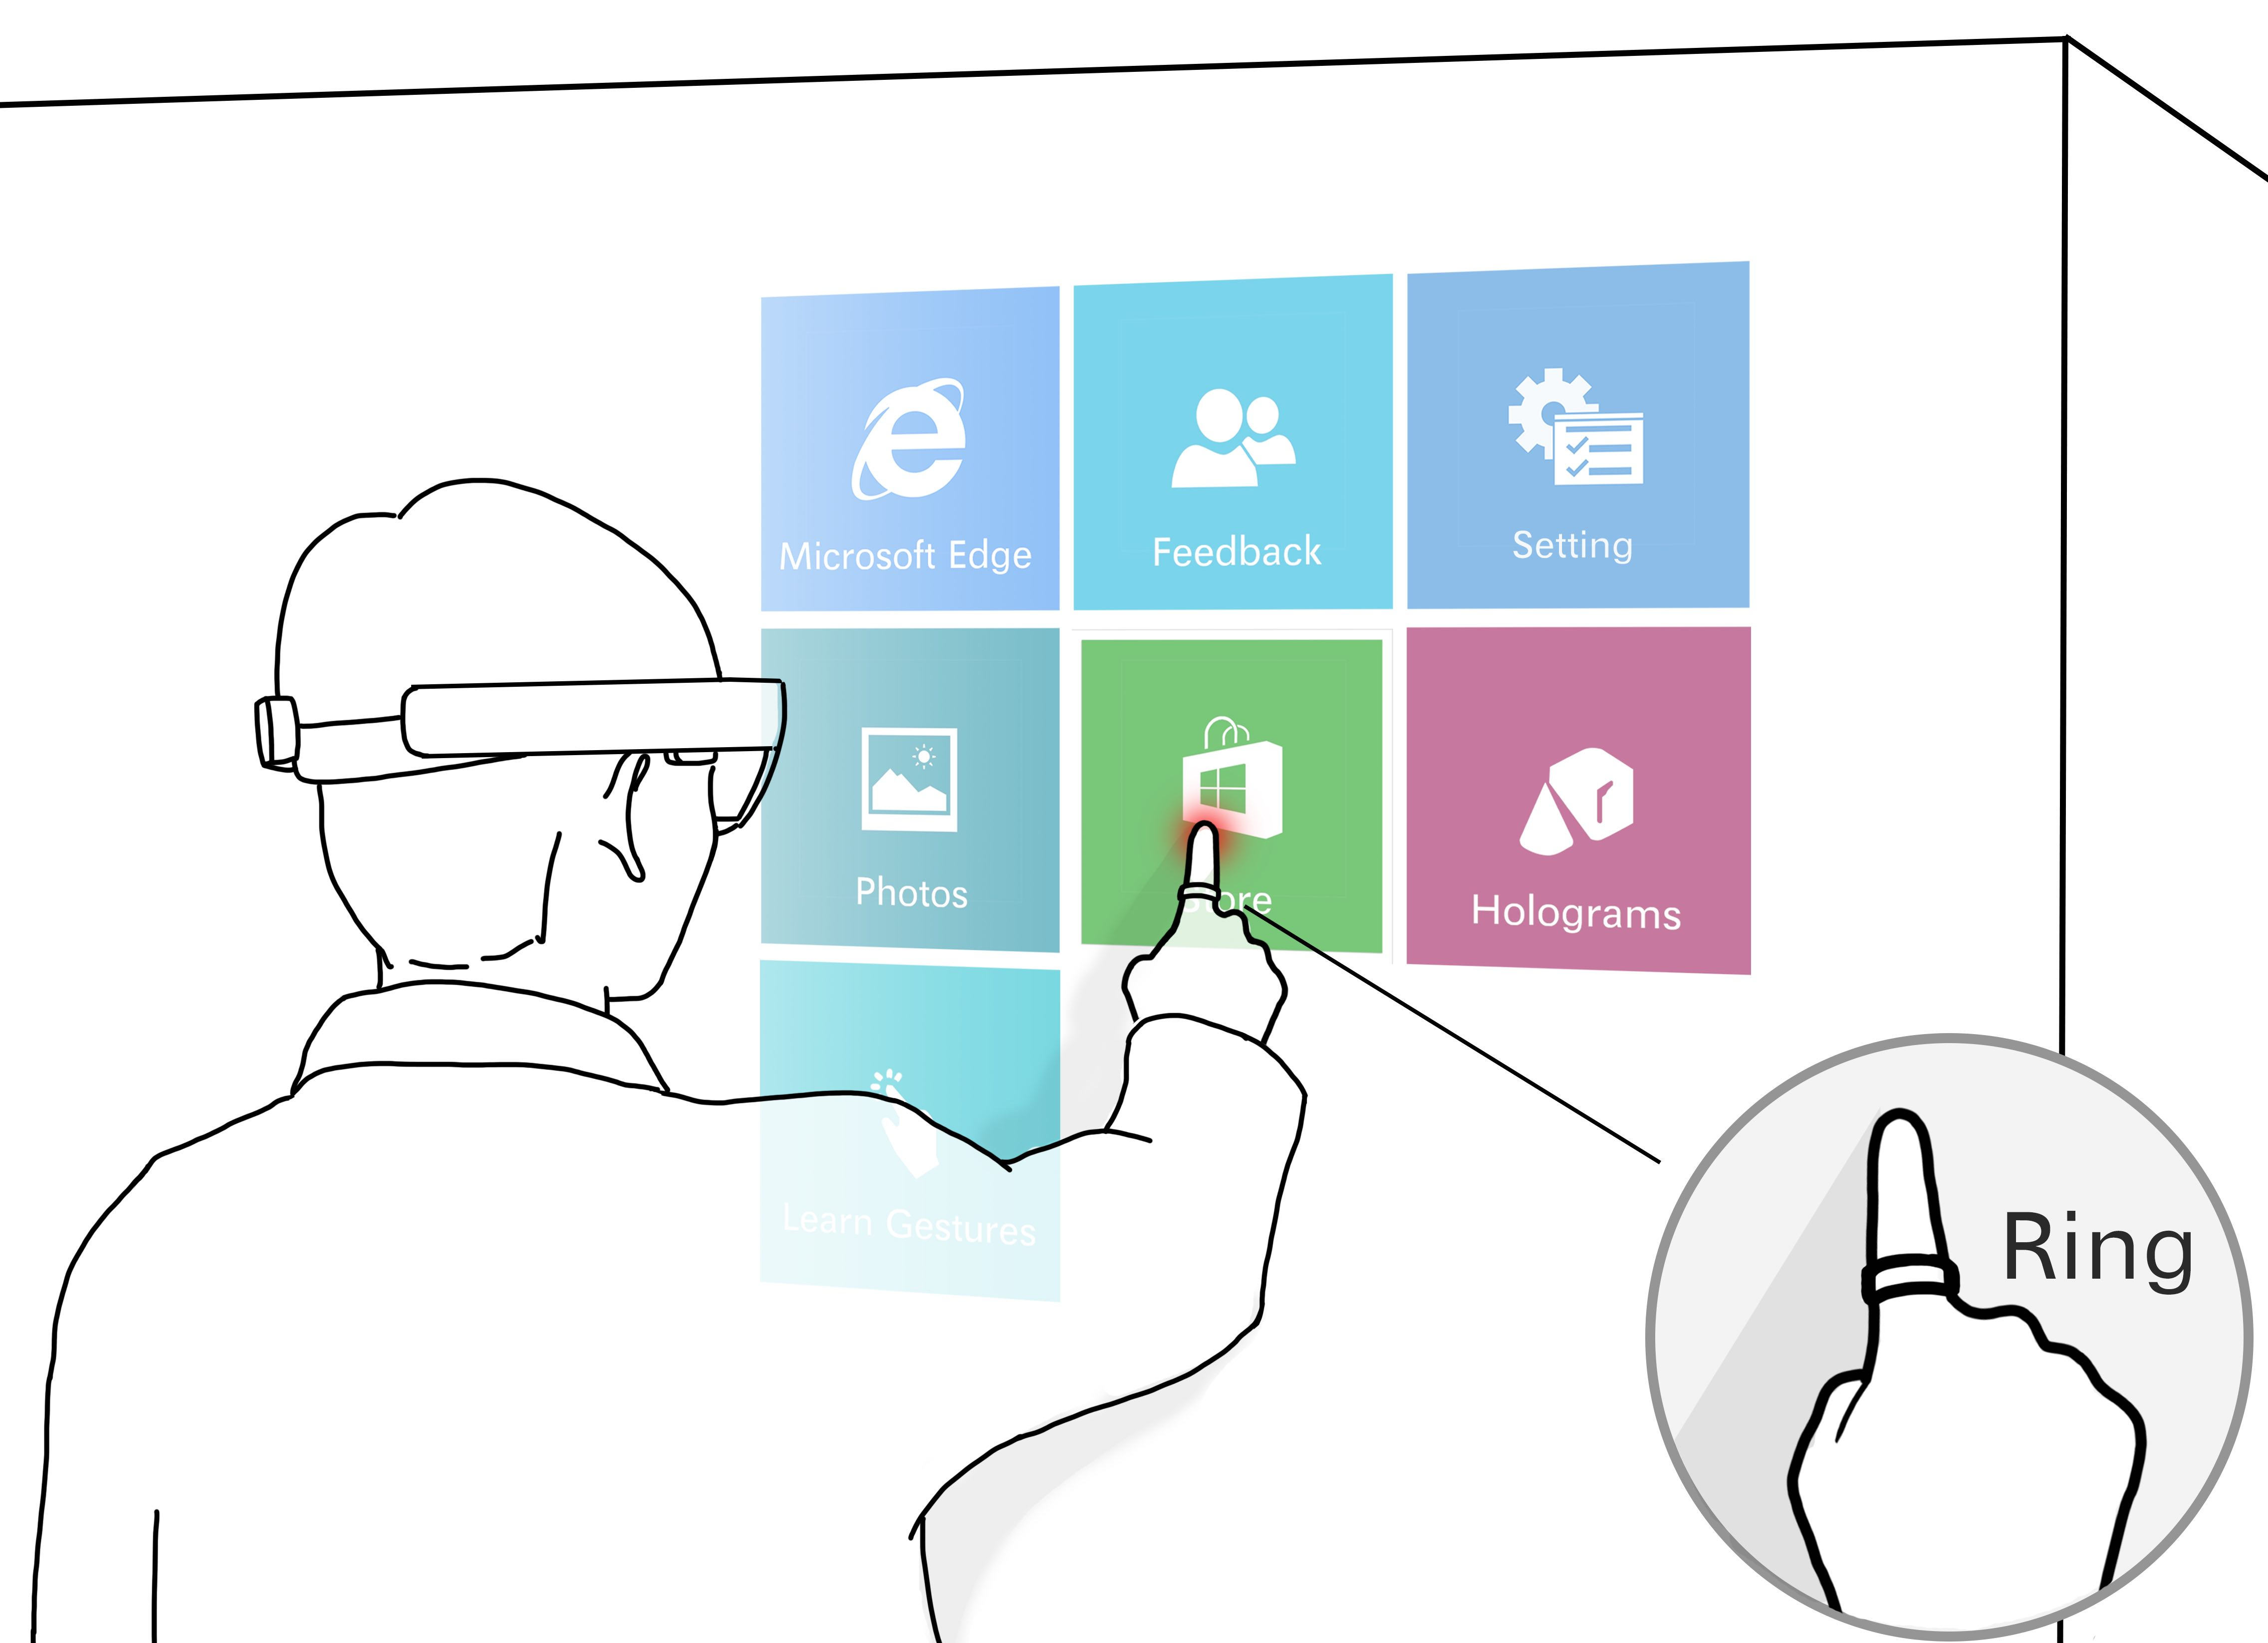
\includegraphics[width=0.8\linewidth]{MR_touch_envision.jpg}
	\caption*{介绍}
	\caption{名称}
	\label{fig:MR_touch_envision}
\end{figure}


\subsection{触摸交互的改进方向}

尽管触摸屏技术已经问世数十年,技术得到了长足的发展,但触摸交互仍有值得改进的地方,分别体现在普适性、响应性和有意性三个方面。

\textbf{(1)普适性}:普适计算是一个强调和环境融为一体的计算概念,主张计算设备朝小型化、可穿戴的方向发展,直至消失在人们的视线当中,人们能在任何时间、地点,以任何方式与与数字世界交互。在人机交互往普适计算发展的过程中,触摸屏等专用输入设备可能是第一批消失的,此时如何支持触摸交互是值得研究的问题。例如,上一小节中所述的基于MR头盔的触摸交互技术是增强触摸普适性的一个实例。

\textbf{(2)响应性}:人对触摸交互响应性的感官需求极高,在点击触摸任务中,人能察觉到低至10毫秒的端到端延迟,并对高于100毫秒的延迟感到极度厌烦[xx]。然而,目前智能手机触摸屏的延迟普遍在50毫秒以上,未能给用户提供极致的用户体验。一种容易察觉到延迟的方法是快速的拖拽任务,例如,在手机中长按APP图标并快速移动。尽管目前的触摸屏延迟在多数任务下不会让用户感到厌烦,但如果要将用户体验提升到最高水平,就需要将触摸交互的延迟降低到10毫秒以内,让用户无法察觉延迟的存在。

\textbf{(3)意图性}:自然动作交互是人机交互的发展趋势,其特点是有意动作和无意动作混杂,给交互的意图识别带来困难。例如,在目前的触摸屏十指打字中,用户必须将手悬空,久而久之会导致疲劳的问题,这种要求用户故意悬空手部以防止误触的交互方式是不自然的,应该开发一款强力的防误触算法,允许用户在打字的间隙将手指休息在触摸屏上(而不会引发误触);又例如,在上一小节所述的基于MR头盔的触摸交互模态中,用户既可以在普通的桌子上触摸交互,也可能仅仅是将手休息在桌子上,在此场景下的触摸交互技术需要发展出识别用户触摸是否具有交互意图的能力。

改进触摸交互的一条技术路径是充分利用触摸的运动规律,即总结触摸前后手指的位移、速度和加速度特征,建立触摸的运动模型。触摸的运动模型将有利于提高触摸交互的普适性、响应性和有意性,这是因为:(1)基于视觉方法的运动传感是普适计算场景下容易获得的传感能力;(2)触摸运动模型可利用手指触摸表面前的传感信号拟合触摸的运动方程,从而以低延迟、甚至负延迟识别触摸事件;(3)触摸运动方程中的参数将能作为判断触摸有意性的有效特征。

\section{研究现状}

\subsection{电容触摸屏}

很准确、常用,但在普适性、响应性和有意性上存在弊端。

\subsection{基于运动传感的触摸感知技术}

位置识别可以做到很准,但是触摸瞬间的感知是难点。

MR头盔中一种直观的感知触摸事件的方法,是利用MR头盔的前置摄像头来观察用户的手指是否接触到交互表面。然而, 基于视觉的方法在触摸感知方面存在两大内在缺点:首先,由于MR头盔的摄像头是从手背的方向观察手指运动的,手指与交互平面的接触点时常被遮挡,因此很难准确、低延迟地识别触摸事件;第二,基于手型恢复的视觉方法往往会消耗大量的计算资源,导致系统延迟过大,影响用户体验。出于以上原因,此前最先进的利用Hololens识别任意物体表面触摸事件的工作中,实验表面存在3.5\%的未识别点击和19.0\%的误触[xx],系统延迟达到180毫秒。在相关工作中,有许多工作致力于提高触摸的识别准确率[2019-5,31],降低识别延迟[2019-18,43,2,6]。因此,基于视觉的触摸感知技术仍然未达到实用水平,仍然需要进一步改进。

\section{研究内容}

触摸交互是人主动控制手指触摸交互表面,通过点击、长按、滑动、拖拽等手势向计算机输入信息的方式。目前,触摸交互技术的改进难点在于触摸瞬间的识别,是否具有强普适性[]、高响应性[]和准确的有意性[],这要求研究者在触摸前后极短的时间跨度上优化触摸交互技术。在此背景下,本文提出了基于最佳控制理论的触摸运动模型。

触摸运动模型描述了一次触摸中,用户从产生触摸意图,到手指触碰到交互表面这一段短暂时间中的运动规律,时间跨度大约为100毫秒,运动规律包括手指的位移、速度和加速度的时空运动规律。围绕触摸运动模型的建立和应用,我们提出了以下三点研究内容:

\textbf{(1)触摸运动数学模型}:本文中的触摸运动特指从用户产生触摸意图,到手指触碰到交互表面的这一段时间中手指的运动规律,触摸运动的数学模型是描述触摸运动时空轨迹的数学方程$x(t)$,描述手指位置$x$与时间$t$之间的关系。通过对时间$t$求导,该方程可描述手指瞬时速度$v$、加速度$a$与时间$t$之间的关系。本文的第一个研究内容是触摸运动的数学模型是什么,即$x(t)$的表达式具体是什么。

\textbf{(2)触摸运动计算模型}:在已知触摸运动方程的前提下,想要利用模型来改进触摸交互技术,还需要弄清楚一个问题,即如何利用传感信号拟合触摸运动方程。在工程上,有若干传感器种可用于传感手指的运动信号,例如,深度摄像头可以感知手指的位移$x$;戴在手指上的运动传感器可以感知手指的加速度$a$。然而,传感信号并非真值,传感器总是收到采样率和采样精度的限制,在这些限制之下,如何更精准地拟合触摸运动方程,是第二个研究内容——触摸运动计算模型需要回答的问题。

\textbf{(3)模型对触摸交互技术的指导性意义}:触摸运动模型揭示了触摸事件前后手指运动的规律,与触摸交互技术息息相关,在此背景下,如何利用触摸运动模型改进触摸运动交互,是值得研究的内容。

\section{主要研究成果}

本文提出了基于最优控制理论的触摸运动模型,揭示了触摸事件前后极短时间内手指的运动规律,探讨了如何利用触摸传感信号(包括位移、速度和加速度)更准确地拟合触摸运动方程。本文详细描述了触摸运动模型(第2章),讨论了模型对触摸交互技术的指导性意义。基于触摸运动模型,本文针对经典的触摸交互任务(目标选择和文本输入),优化触摸感知(第3章)和意图推理技术(第4章),提升触摸交互的效率和用户体验。

\textbf{(1)提出了基于最佳控制理论的触摸运动模型}

通过实验观察和验证,本文发现,人产生触摸意图时,已对触摸运动做出了完整的规划,其心理可描述为:\emph{“在规定时间$t_1$内,最平稳地将手指从初始点$x_0$移动到目标点$x_1$。”}其中,目标点$x_1$是位于交互表面之下的虚构点。在触碰到交互表面之前,手指会沿着最平稳的时空轨迹向目标点$x_1$移动,直到接触交互表面而停止。根据Tamar等人关于最佳控制理论适用于手部运动建模的论述[xx],“最平稳的”指的是最小化手指运动急动度的平方的积分,由此约束可解得触摸运动的方程如下所示:

\begin{equation}
x(\tau)=
\begin{cases}
x_0+(x_1-x_0)(6\tau^5-15\tau^4+10\tau^3)& \tau<=\tau_c \\
0& \tau>\tau_c
\end{cases}
\end{equation}

其中,$\tau=\frac{t}{t1}$是运动的时间进度,$\tau_c$表示手指触摸到交互表面的时间。以上是触摸运动模型的数学模型部分。

在工程技术中,只有对触摸运动方程进行有效的拟合,才能充分发挥模型的作用。本文提出了触摸运动的计算模型,提出了利用运动传感信号更准确地拟合触摸运动方程的计算方法。本文讨论了各运动传感信道(位移、速度、加速度)、传感精度和采样率对运动方程拟合精度的影响。最后,本文讨论了模型对触摸交互技术的指导性意义,包括(1)低延迟触摸感知,(2)防误触技术,(3)触摸瞬间力度估计,和(4)运动传感器性能改进建议。其中,低延迟触摸感知技术和防误触技术具有重要的实用价值,为此,作者基于模型实现了对这两项交互技术的优化,做出后续两点主要贡献:

\textbf{(2)提出了基于运动传感指环的低延迟触摸感知技术:}

针对现有触摸感知技术普适性不强,响应性不高的问题,本文提出了基于运动传感指环的低延迟触摸感知技术。目前主流的电容触摸屏技术存在普适性不强的缺点,用户只能在专用触摸屏设备上进行触摸交互,不符合普适计算中随时、随地、随心交互的原则。xx等人提出了基于运动传感指环的触摸感知技术,使得用户能在无源物体表面(如桌面、墙面)上触摸输入,增强了触摸交互的普适性。然而,先前基于运动传感指环的技术采用阈值方法判断触摸事件,延迟高达200毫秒,准确率仅为85\%,不满足触摸交互的高响应性需求。

基于触摸运动模型,本提出了基于运动传感指环的低延迟触摸感知技术。从信息论的角度能够论证,基于触摸运动模型的触摸感知技术最大限度地利用了传感器所提供的信息,其感知能力远优于先前工作中所使用的阈值方法或机器学习方法,通过实验我们也验证了这一观点:本技术的触摸感知延迟低至10毫秒,准确率超过99\%。低延迟是本技术的关键词,由于人在触摸交互中无法察觉到10毫秒的延迟,本技术为用户提供了最佳用户体验,与先前技术相比实现了质的飞越。

在触摸感知的基础上,本文介绍了一种基于运动传感指环的单指文本输入法,用户可以在普通的桌子上打字,速度达到每分钟输入20.59个英文单词。该文本输入技术为混合现实场景提供了高效、实用的文本输入方案。鉴于文本输入是最复杂的触摸输入任务之一,该文本输入技术的成功验证了低延迟触摸感知技术的鲁棒性。

\textbf{(3)提出了面向连续触摸输入的防误触技术:}

针对现有触摸屏设备上,连续触摸输入误触频发的问题,本文提出了基于触摸运动模型的防误触技术。触摸屏文本输入是典型的连续触摸任务,是最复杂的触摸交互任务之一。目前,用户在触摸屏上十指打字时需要将手指悬空,以避免误触发生,久而久之会产生疲劳的问题;而若用户不将手指悬空,则手指在贴近触摸屏时会引发误触。

解决上述问题最直接的方法是开发一款强力的防误触技术,让用户在触摸屏十指打字的间隙可以将手指休息在屏幕上,而不引发误触,系统只对表达打字意图的触摸做出响应。通过实验观察和数据分析,作者发现:(1)同样是手指触摸屏幕,有意触摸和误触在触摸运动方程的参数上是有差异的,触摸的速度、力度、时长都是触摸有意性的重要表征;(2)有意触摸中,手指触摸运动方程的参数与其它手指独立,而多指休息导致的误触中,不同手指的触摸运动方程的参数具有强相关性。结合以上规律,作者提出了面向连续触摸输入的防误触技术,识别准确率达到99\%,且允许用户在十指打字的间隙将手指休息在触摸屏上(而不会引发误触)。实验表明,该技术改变了用户的打字行为,用户将手指休息在触摸屏上,打字行为更自然、更抗疲劳,打字速度也提升了20\%。

\section{论文组织结构}

本文后续章节的组织结构如下:

第2章介绍了基于最优控制理论的触摸运动模型,包括触摸运动的数学建模、计算建模、推导过程和实验评估,并讨论了触摸运动模型对改进触摸交互技术的指导性意义。

第3章介绍了基于运动传感指环的低延迟触摸感知技术,包括触摸的运动传感信号分析、基于模型的触摸感知技术介绍、针对目标选取任务的用户实验评估、基于指环触摸感知的文本输入技术介绍,和针对文本输入任务的用户实验评估。

第4章介绍了面向连续触摸输入的防误触技术,包括连续触摸输入中有意点击行为和误触行为分析、基于模型的防误触技术介绍、基于防误触技术的有触觉反馈的触屏文本输入技术介绍,以及针对文本输入任务的用户实验评估。

第5章对本文内容进行总结和展望。

\iffalse

\section{插图}

图片通常在 \env{figure} 环境中使用 \cs{includegraphics} 插入,如图~\ref{fig:example} 的源代码。
建议矢量图片使用 PDF 格式,比如数据可视化的绘图;
照片应使用 JPG 格式;
其他的栅格图应使用无损的 PNG 格式。
注意,LaTeX 不支持 TIFF 格式;EPS 格式已经过时。

\begin{figure}
	\centering
	
\includegraphics[width=0.5\linewidth]{example-image-a.pdf}
	\caption*{国外的期刊习惯将图表的标题和说明文字写成一段,需要改写为标题只含图表的名称,其他说明文字以注释方式写在图表下方,或者写在正文中。}
	\caption{示例图片标题}
	\label{fig:example}
\end{figure}

若图或表中有附注,采用英文小写字母顺序编号,附注写在图或表的下方。
国外的期刊习惯将图表的标题和说明文字写成一段,需要改写为标题只含图表的名称,其他说明文字以注释方式写在图表下方,或者写在正文中。

如果一个图由两个或两个以上分图组成时,各分图分别以 (a)、(b)、(c)...... 作为图序,并须有分图题。
推荐使用 \pkg{subcaption} 宏包来处理, 比如图~\ref{fig:subfig-a} 和图~\ref{fig:subfig-b}。

\begin{figure}
	\centering
	\subcaptionbox{分图 A\label{fig:subfig-a}}
	{
\includegraphics[width=0.35\linewidth]{example-image-a.pdf}}
	\subcaptionbox{分图 B\label{fig:subfig-b}}
	{
\includegraphics[width=0.35\linewidth]{example-image-b.pdf}}
	\caption{多个分图的示例}
	\label{fig:multi-image}
\end{figure}



\section{表格}

表应具有自明性。为使表格简洁易读,尽可能采用三线表,如表~\ref{tab:three-line}。
三条线可以使用 \pkg{booktabs} 宏包提供的命令生成。

\begin{table}
	\centering
	\caption{三线表示例}
	\begin{tabular}{ll}
		\toprule
		文件名          & 描述                         \\
		\midrule
		thuthesis.dtx   & 模板的源文件,包括文档和注释 \\
		thuthesis.cls   & 模板文件                     \\
		thuthesis-*.bst & BibTeX 参考文献表样式文件    \\
		\bottomrule
	\end{tabular}
	\label{tab:three-line}
\end{table}

表格如果有附注,尤其是需要在表格中进行标注时,可以使用 \pkg{threeparttable} 宏包。
研究生要求使用英文小写字母 a、b、c……顺序编号,本科生使用圈码 ①、②、③……编号。

\begin{table}
	\centering
	\begin{threeparttable}[c]
		\caption{带附注的表格示例}
		\label{tab:three-part-table}
		\begin{tabular}{ll}
			\toprule
			文件名                 & 描述                         \\
			\midrule
			thuthesis.dtx\tnote{a} & 模板的源文件,包括文档和注释 \\
			thuthesis.cls\tnote{b} & 模板文件                     \\
			thuthesis-*.bst        & BibTeX 参考文献表样式文件    \\
			\bottomrule
		\end{tabular}
		\begin{tablenotes}
			\item [a] 可以通过 xelatex 编译生成模板的使用说明文档;
			使用 xetex 编译 \file{thuthesis.ins} 时则会从 \file{.dtx} 中去除掉文档和注释,得到精简的 \file{.cls} 文件。
			\item [b] 更新模板时,一定要记得编译生成 \file{.cls} 文件,否则编译论文时载入的依然是旧版的模板。
		\end{tablenotes}
	\end{threeparttable}
\end{table}

如某个表需要转页接排,可以使用 \pkg{longtable} 宏包,需要在随后的各页上重复表的编号。
编号后跟表题(可省略)和“(续)”,置于表上方。续表均应重复表头。

\begin{longtable}{cccc}
	\caption{跨页长表格的表题} \\
	\toprule
	表头 1 & 表头 2 & 表头 3 & 表头 4 \\
	\midrule
	\endfirsthead
	\caption[]{跨页长表格的表题(续)} \\
	\toprule
	表头 1 & 表头 2 & 表头 3 & 表头 4 \\
	\midrule
	\endhead
	\bottomrule
	\endfoot
	Row 1  & & & \\
	Row 2  & & & \\
	Row 3  & & & \\
	Row 4  & & & \\
	Row 5  & & & \\
	Row 6  & & & \\
	Row 7  & & & \\
	Row 8  & & & \\
	Row 9  & & & \\
	Row 10 & & & \\
\end{longtable}



\section{算法}

算法环境可以使用 \pkg{algorithms} 或者 \pkg{algorithm2e} 宏包。

\renewcommand{\algorithmicrequire}{\textbf{输入:}\unskip}
\renewcommand{\algorithmicensure}{\textbf{输出:}\unskip}

\begin{algorithm}
	\caption{Calculate $y = x^n$}
	\label{alg1}
	\small
	\begin{algorithmic}
		\REQUIRE $n \geq 0$
		\ENSURE $y = x^n$
		
		\STATE $y \leftarrow 1$
		\STATE $X \leftarrow x$
		\STATE $N \leftarrow n$
		
		\WHILE{$N \neq 0$}
		\IF{$N$ is even}
		\STATE $X \leftarrow X \times X$
		\STATE $N \leftarrow N / 2$
		\ELSE[$N$ is odd]
		\STATE $y \leftarrow y \times X$
		\STATE $N \leftarrow N - 1$
		\ENDIF
		\ENDWHILE
	\end{algorithmic}
\end{algorithm}


模板支持 BibTeX 和 BibLaTeX 两种方式处理参考文献。
下文主要介绍 BibTeX 配合 \pkg{natbib} 宏包的主要使用方法。


\section{顺序编码制}

在顺序编码制下,默认的 \cs{cite} 命令同 \cs{citep} 一样,序号置于方括号中,
引文页码会放在括号外。
统一处引用的连续序号会自动用短横线连接。

\thusetup{
	cite-style = super,
}
\begin{tabular}{l@{\quad$\Rightarrow$\quad}l}
	\verb|\cite{zhangkun1994}|               & \cite{zhangkun1994}               \\
	\verb|\citet{zhangkun1994}|              & \citet{zhangkun1994}              \\
	\verb|\citep{zhangkun1994}|              & \citep{zhangkun1994}              \\
	\verb|\cite[42]{zhangkun1994}|           & \cite[42]{zhangkun1994}           \\
	\verb|\cite{zhangkun1994,zhukezhen1973}| & \cite{zhangkun1994,zhukezhen1973} \\
\end{tabular}


也可以取消上标格式,将数字序号作为文字的一部分。
建议全文统一使用相同的格式。

\thusetup{
	cite-style = inline,
}
\begin{tabular}{l@{\quad$\Rightarrow$\quad}l}
	\verb|\cite{zhangkun1994}|               & \cite{zhangkun1994}               \\
	\verb|\citet{zhangkun1994}|              & \citet{zhangkun1994}              \\
	\verb|\citep{zhangkun1994}|              & \citep{zhangkun1994}              \\
	\verb|\cite[42]{zhangkun1994}|           & \cite[42]{zhangkun1994}           \\
	\verb|\cite{zhangkun1994,zhukezhen1973}| & \cite{zhangkun1994,zhukezhen1973} \\
\end{tabular}



\section{著者-出版年制}

著者-出版年制下的 \cs{cite} 跟 \cs{citet} 一样。

\thusetup{
	cite-style = author-year,
}
\begin{tabular}{l@{\quad$\Rightarrow$\quad}l}
	\verb|\cite{zhangkun1994}|                & \cite{zhangkun1994}                \\
	\verb|\citet{zhangkun1994}|               & \citet{zhangkun1994}               \\
	\verb|\citep{zhangkun1994}|               & \citep{zhangkun1994}               \\
	\verb|\cite[42]{zhangkun1994}|            & \cite[42]{zhangkun1994}            \\
	\verb|\citep{zhangkun1994,zhukezhen1973}| & \citep{zhangkun1994,zhukezhen1973} \\
\end{tabular}

\vskip 2ex
\thusetup{
	cite-style = super,
}
注意,引文参考文献的每条都要在正文中标注
\cite{zhangkun1994,zhukezhen1973,dupont1974bone,zhengkaiqing1987,%
	jiangxizhou1980,jianduju1994,merkt1995rotational,mellinger1996laser,%
	bixon1996dynamics,mahui1995,carlson1981two,taylor1983scanning,%
	taylor1981study,shimizu1983laser,atkinson1982experimental,%
	kusch1975perturbations,guangxi1993,huosini1989guwu,wangfuzhi1865songlun,%
	zhaoyaodong1998xinshidai,biaozhunhua2002tushu,chubanzhuanye2004,%
	who1970factors,peebles2001probability,baishunong1998zhiwu,%
	weinstein1974pathogenic,hanjiren1985lun,dizhi1936dizhi,%
	tushuguan1957tushuguanxue,aaas1883science,fugang2000fengsha,%
	xiaoyu2001chubanye,oclc2000about,scitor2000project%
}。


\section{数学符号}

中文论文的数学符号默认遵循 GB/T 3102.11—1993《物理科学和技术中使用的数学符号》
\footnote{原 GB 3102.11—1993,自 2017 年 3 月 23 日起,该标准转为推荐性标准。}。
该标准参照采纳 ISO 31-11:1992 \footnote{目前已更新为 ISO 80000-2:2019。},
但是与 \TeX{} 默认的美国数学学会(AMS)的符号习惯有所区别。
具体地来说主要有以下差异:
\begin{enumerate}
	\item 大写希腊字母默认为斜体,如
	\begin{equation*}
		\Gamma \Delta \Theta \Lambda \Xi \Pi \Sigma \Upsilon \Phi \Psi \Omega.
	\end{equation*}
	注意有限增量符号 $\increment$ 固定使用正体,模板提供了 \cs{increment} 命令。
	\item 小于等于号和大于等于号使用倾斜的字形 $\le$、$\ge$。
	\item 积分号使用正体,比如 $\int$、$\oint$。
	\item 行间公式积分号的上下限位于积分号的上下两端,比如
	\begin{equation*}
		\int_a^b f(x) \dif x.
	\end{equation*}
	行内公式为了版面的美观,统一居右侧,如 $\int_a^b f(x) \dif x$ 。
	\item
	偏微分符号 $\partial$ 使用正体。
	\item
	省略号 \cs{dots} 按照中文的习惯固定居中,比如
	\begin{equation*}
		1, 2, \dots, n \quad 1 + 2 + \dots + n.
	\end{equation*}
	\item
	实部 $\Re$ 和虚部 $\Im$ 的字体使用罗马体。
\end{enumerate}

以上数学符号样式的差异可以在模板中统一设置。
另外国标还有一些与 AMS 不同的符号使用习惯,需要用户在写作时进行处理:
\begin{enumerate}
	\item 数学常数和特殊函数名用正体,如
	\begin{equation*}
		\uppi = 3.14\dots; \quad
		\symup{i}^2 = -1; \quad
		\symup{e} = \lim_{n \to \infty} \left( 1 + \frac{1}{n} \right)^n.
	\end{equation*}
	\item 微分号使用正体,比如 $\dif y / \dif x$。
	\item 向量、矩阵和张量用粗斜体(\cs{symbf}),如 $\symbf{x}$、$\symbf{\Sigma}$、$\symbfsf{T}$。
	\item 自然对数用 $\ln x$ 不用 $\log x$。
\end{enumerate}


英文论文的数学符号使用 \TeX{} 默认的样式。
如果有必要,也可以通过设置 \verb|math-style| 选择数学符号样式。

关于量和单位推荐使用
\href{http://mirrors.ctan.org/macros/latex/contrib/siunitx/siunitx.pdf}{\pkg{siunitx}}
宏包,
可以方便地处理希腊字母以及数字与单位之间的空白,
比如:
\SI{6.4e6}{m},
\SI{9}{\micro\meter},
\si{kg.m.s^{-1}},
\SIrange{10}{20}{\degreeCelsius}。

\section{数学公式}

数学公式可以使用 \env{equation} 和 \env{equation*} 环境。
注意数学公式的引用应前后带括号,建议使用 \cs{eqref} 命令,比如式\eqref{eq:example}。
\begin{equation}
	\frac{1}{2 \uppi \symup{i}} \int_\gamma f = \sum_{k=1}^m n(\gamma; a_k) \mathscr{R}(f; a_k)
	\label{eq:example}
\end{equation}
注意公式编号的引用应含有圆括号,可以使用 \cs{eqref} 命令。

多行公式尽可能在“=”处对齐,推荐使用 \env{align} 环境。
\begin{align}
	a & = b + c + d + e \\
	& = f + g
\end{align}



\section{数学定理}

定理环境的格式可以使用 \pkg{amsthm} 或者 \pkg{ntheorem} 宏包配置。
用户在导言区载入这两者之一后,模板会自动配置 \env{thoerem}、\env{proof} 等环境。

\begin{theorem}[Lindeberg--Lévy 中心极限定理]
	设随机变量 $X_1, X_2, \dots, X_n$ 独立同分布, 且具有期望 $\mu$ 和有限的方差 $\sigma^2 \ne 0$,
	记 $\bar{X}_n = \frac{1}{n} \sum_{i+1}^n X_i$,则
	\begin{equation}
		\lim_{n \to \infty} P \left(\frac{\sqrt{n} \left( \bar{X}_n - \mu \right)}{\sigma} \le z \right) = \Phi(z),
	\end{equation}
	其中 $\Phi(z)$ 是标准正态分布的分布函数。
\end{theorem}
\begin{proof}
	Trivial.
\end{proof}

同时模板还提供了 \env{assumption}、\env{definition}、\env{proposition}、
\env{lemma}、\env{theorem}、\env{axiom}、\env{corollary}、\env{exercise}、
\env{example}、\env{remar}、\env{problem}、\env{conjecture} 这些相关的环境。

\fi
% !TeX root = ../thuthesis-example.tex

\chapter{基于最优控制理论的触摸运动模型}

最优控制理论是数学最优化的分支,研究使动力控制系统的性能指标实现最优化的综合方法。自1962年Potryagin等人提出最优控制理论以来[xx],该理论被广泛应用于空间技术[]、电力系统控制[]、经济调控[]等重要领域。1985年,Tamar等人指出,最优控制理论还可用于描述人的手部运动过程[xx]。论文指出,人在手部运动的控制过程中,大脑并不会具体地控制肩关节和肘关节的旋转角度,而是将注意力集中在手部(由手掌和手指构成的整体),试图“\emph{在规定时间$t_1$内,最平稳地将手部从初始点$(x_0, y_0, z_0)$移动到目标点$(x_f, y_f, z_f)$}”。其中,“最平稳地”指的是人下意识地最小化手了部运动急动度平方的积分:

\begin{equation}
	C=\frac{1}{2}\int_{0}^{t_1}\left(\left(\frac{d^3x}{dt^3}\right)^2+\left(\frac{d^3y}{dt^3}\right)^2+\left(\frac{d^3z}{dt^3}\right)^2\right)dt
	\label{equ:objective_function}
\end{equation}

其中,$x(t)$,$y(t)$和$z(t)$是手部位置随时间变化的函数。受到这份工作的启发,本文作者通过实验验证发现,触摸运动过程同样可由公式\ref{equ:objective_function}描述。在此公式的约束下,本文提出了基于最优控制理论的触摸运动模型。本章分三部分介绍触摸运动模型:(1)触摸运动的数学模型,即描述触摸运动过程的数学方程;(2)触摸运动的计算模型,即利用运动传感信号(位移、速度、加速度时间序列)拟合触摸运动方程的最优化方法;(3)模型对触摸交互技术的指导性意义,即探讨触摸运动方程能给触摸交互技术带来哪些有用的信息,及如何利用这些信息改进交互技术。

\section{触摸运动的数学模型}

触摸运动的数学模型是描述触摸事件前后短暂时间内手指运动过程的数学方程。触摸运动的过程可描述为:“\emph{如图\ref{fig:touch_model_virtual}所示,若交互表面凭空消失,人会在时间$t_1$内最平稳地将手指从初始点$x_0$移动到目标点$x_1$。但实际情况是如图\ref{fig:touch_model_real}所示的情况,交互表面真实存在,手指会在时间点$t_c$因与交互表面接触而停止。}”,触摸运动的方程是:

\begin{figure}
	\centering
	\begin{subfigure}[b]{0.45\textwidth}
		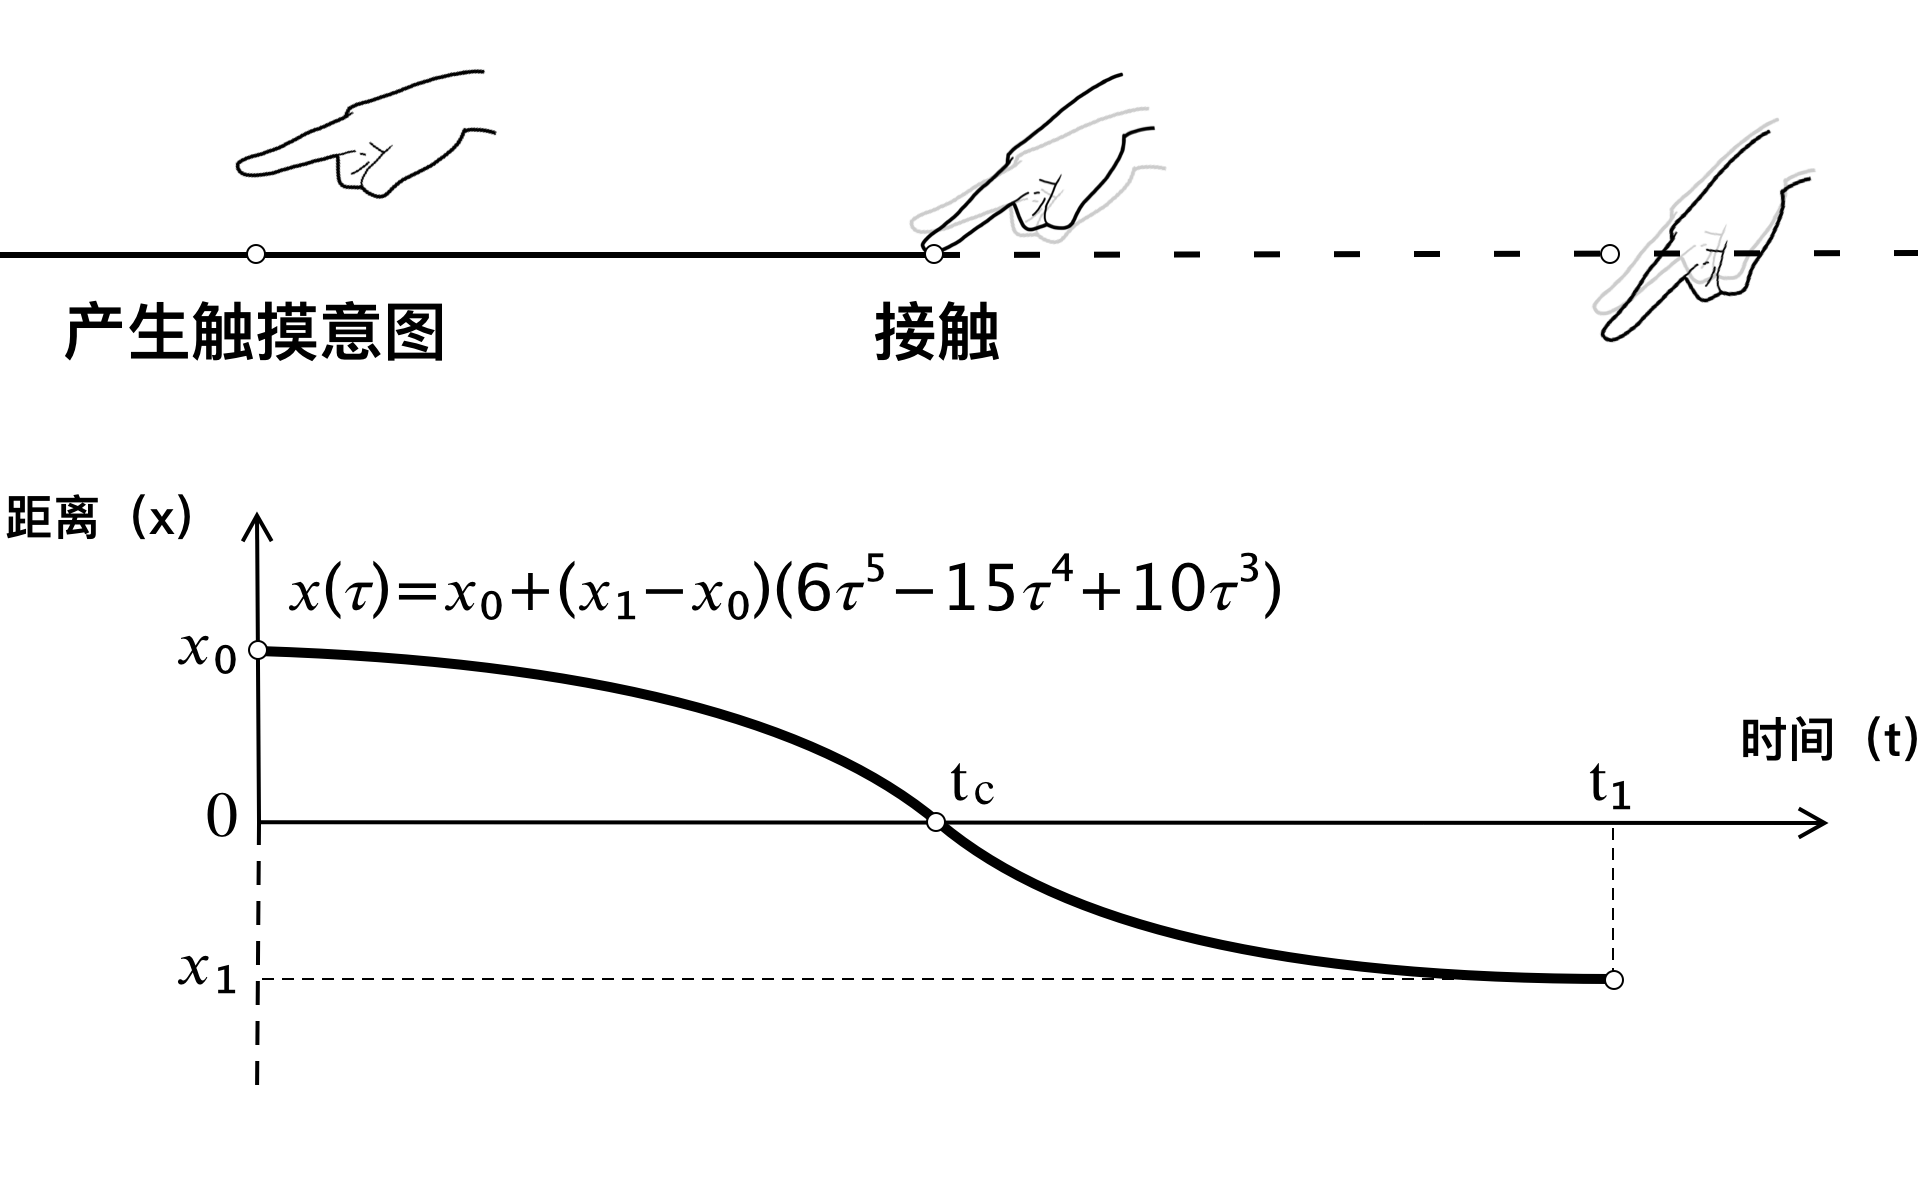
\includegraphics[width=\textwidth]{touch_model_virtual.png}
		\caption{若交互表面凭空消失}
		\label{fig:touch_model_virtual}
	\end{subfigure}\hfill% or \hspace{5mm} or \hspace{0.3\textwidth}
	\begin{subfigure}[b]{0.45\textwidth}
		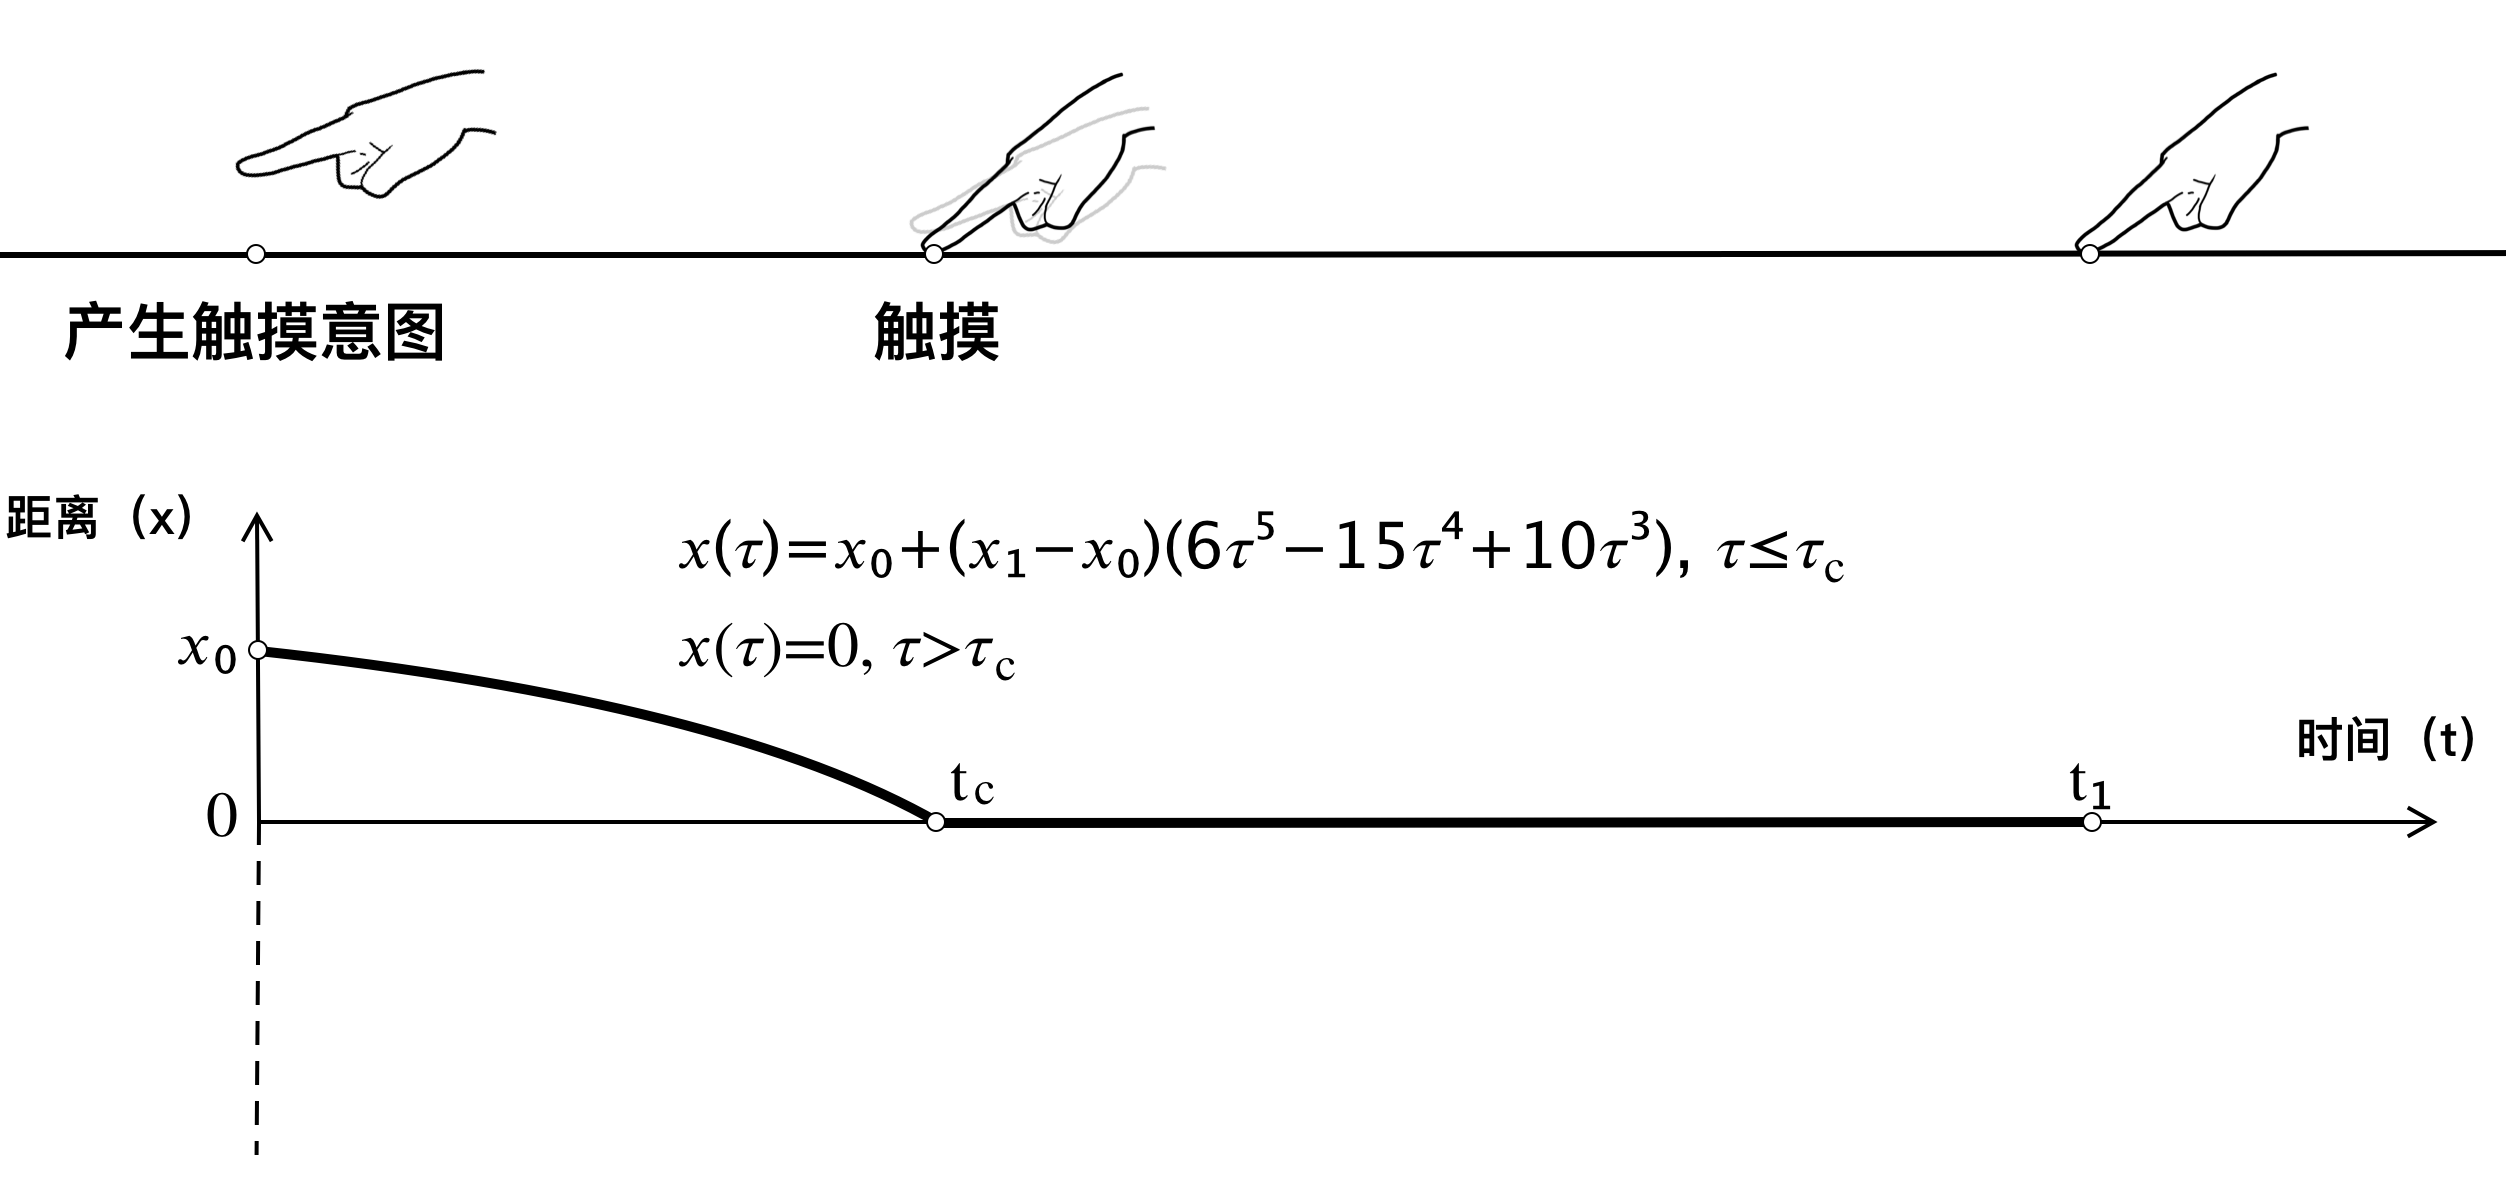
\includegraphics[width=\textwidth]{touch_model_real.png}
		\caption{实际情况}
		\label{fig:touch_model_real}
	\end{subfigure}
	\caption{基于最佳控制理论的触摸运动模型图示}
	\label{fig:touch_model}
\end{figure}

\begin{equation}
	x(\tau)=
	\begin{cases}
		x_0+(x_1-x_0)(6\tau^5-15\tau^4+10\tau^3)& \tau<=\tau_c \\
		0& \tau>\tau_c
	\end{cases}
\label{equ:touch_model}
\end{equation}

其中,$x$是手指与交互表面的高度之差,$\tau=\frac{t}{t1}$是时间进度。通过对上述函数的求导不难发现,触摸运动模型同时揭示了手指速度$v$和加速度$a$与时间$t$之间的关系:

\begin{equation}
v(\tau)=
\begin{cases}
	(x_1-x_0)(30\tau^4-60\tau^3+30\tau^2)& \tau<\tau_c \\
	0& \tau>\tau_c
\end{cases}
\end{equation}

\begin{equation}
	a(\tau)=
	\begin{cases}
		(x_1-x_0)(120\tau^3-180\tau^2+60\tau)& \tau<\tau_c \\
		0& \tau>\tau_c
	\end{cases}
\label{equ:touch_model_a}
\end{equation}

公式\ref{equ:touch_model}即为触摸运动的数学模型,本小节剩余内容将介绍模型的提出和推导过程。需要声明的是,本文提出的触摸运动模型是对触摸运动过程的良好拟合,后续章节会通过用户实验验证模型的预测精度。然而,同人机交互中许多经典的模型一样(如费茨定理[xx]),本模型的正确性是无法从人体机理的角度证明的,模型有可能在未来工作中会得到修正和完善。

本文中,触摸运动模型的提出源于一个非正式实验。如图xx所示,16名被试参与了实验,被试用食指连续地点击一块木板,实验者使用300Hz的高速摄像头记录被试手指的运动过程。在被试连续点击数次之后,实验者要求被试闭上双眼,继续点击。实验者在数秒后迅速移开木板,这一次,被试的手指触摸运动会“踏空”,实验也随即结束。每名用户只会进行一次实验,采集一次手指踏空的数据,而不会重复实验,这是为了防止用户知道实验意图之后,其触摸心理发生改变。高速摄像头记录的数据显示,在被试手指踏空的触摸运动中,其手指移动到了位于原来木板表面的高度之下,约1到3厘米的位置上。实验表明,人在组织一次触摸时,其心理并非将手指从初始点带到交互表面上,而是将手指带到交互表面之下的一个虚构点上。

【图:手指踏空实验】

根据最优控制理论,用户组织触摸运动的心理可描述为:“在规定时间$t_1$内,最平稳地将手部从初始点$(x_0, y_0, z_0)$移动到目标点$(x_1, y_1, z_1)$。”其中,“最平稳地”指的是最小化手指运动急动度的平方的积分(公式\ref{equ:objective_function})。为了简化触摸运动方程,作者假设手指在触摸运动的初始点和目标点上都是静止的,即速度和加速度同时为零。该假设是近似的,是考虑到当前传感器精度有限而做出的折中的约束条件,这是因为,如果运动方程的约束条件太少,运动方程的未知变量会变多,使得实际工程项目中很难以有限的运动传感精度和采样率拟合出准确的触摸运动轨迹。综上所述,若交互表面凭空消失,求解触摸运动方程等价于以下最优化问题:

\begin{equation}
	\begin{cases}
		x(t),y(t),z(t) \\
		s.t. x(0)=x_0,x^{'}(0)=x^{''}(0)=0,x(t_1)=x_1,x^{'}(t_1)=x^{''}(t_1)=0 \\
		y(0)=y_0,y^{'}(0)=y^{''}(0)=0,y(t_1)=y_1,y^{'}(t_1)=y^{''}(t_1)=0 \\
		z(0)=x_0,z^{'}(0)=x^{''}(0)=0,z(t_1)=z_1,z^{'}(t_1)=z^{''}(t_1)=0 \\
		min\frac{1}{2}\int_{0}^{t_1}\left(\left(\frac{d^3x}{dt^3}\right)^2+\left(\frac{d^3y}{dt^3}\right)^2+\left(\frac{d^3z}{dt^3}\right)^2\right)dt
	\end{cases}
\end{equation}

读者可能注意到,手部运动应该受到人的运动能力的限制,比如手部运动存在一个速度或加速度的上限。然而,上述最优化问题未包含对运动能力作出条件约束,这是因为,该问题的解天然地不会产生超出手部运动能力限制的情况[xx]。作者将上述最优化问题的求解过程写在附录xx中,此处直接给出问题的解:

\begin{equation}
	\begin{cases}
		x(\tau)=x_0+(x_1-x_0)(6\tau^5-15\tau^4+10\tau^3) \\
		y(\tau)=y_0+(y_1-y_0)(6\tau^5-15\tau^4+10\tau^3) \\
		z(\tau)=z_0+(z_1-z_0)(6\tau^5-15\tau^4+10\tau^3)
	\end{cases}
\end{equation}

上述公式表明,在触摸运动方程中,手指在$x$、$y$、$z$三个轴上的时空运动轨迹是相互独立的。本文在选题背景中已经阐述,本文的研究重点在于提高触摸交互的普适性、响应性和有意性,而不关心触摸在交互表面上2D位置的识别,因此,我们仅保留上述公式中$x$轴上的时空轨迹函数,作为触摸运动模型的表述(公式\ref{equ:touch_model})。

\section{触摸运动的计算模型}

触摸运动的计算模型是在已知数学模型的情况下,利用位移、速度、加速度等传感器信号来拟合触摸运动方程参数的计算方法。在工程技术中,常见的运动信号传感方法主要有(1)基于视觉方法的位移传感,和(2)基于运动传感器的加速度传感。由于速度传感器大多通过位移除以时间来计算,本文只讨论位移信号,而省去速度信号。

实验观察发现,一次触摸运动从用户产生触摸意图(手指开始加速运动),到手指触碰到交互表面的时长最短不低于50毫秒,最长不超过200毫秒。因此,从实用的角度出发,触摸运动的计算模型应该讨论,如何利用触摸事件发生前50毫秒的采样数据拟合触摸运动方程。假设我们用采样频率为$f_x$的位移传感器和采样频率为$f_a$的加速度传感器监测手指运动,在触摸发生前50毫秒内收集到以下数据:

\begin{equation}
\begin{cases}
[X_1, X_2, \cdots, X_n]& n=\lfloor0.05f_x\rfloor \\
[A_1, A_2, \cdots, A_m]& m=\lfloor0.05f_a\rfloor
\end{cases}
\end{equation}

则触摸运动的计算模型是利用上述时间序列拟合触摸运动方程(公式\ref{equ:touch_model})的计算方法。本小节剩余内容将按照计算顺序介绍此问题的解决方法。

\subsection{卡尔曼滤波}

卡尔曼滤波可用于控制测量数据的误触。研究工作中一般认为,基于视觉方法的位移信号和基于运动传感器的加速度信号的传感误差都符合正态分布[xx],设位移信号的标准差为$\sigma_x$,加速度信号的标准差为$\sigma_a$。$\sigma_x$和$\sigma_a$的值取决于传感器的质量,可以通过实验测量。

卡尔曼滤波器如何设计。

由于卡尔曼滤波联立了位移信号和加速度信号,最终可以将位移传感信号的误差降低至$\bigtriangleup x=k_x\sigma_x$,将加速度传感信号的误差降低至$\bigtriangleup a=k_a\sigma_a$。

\subsection{最小二乘拟合}

拟合触摸运动方程的过程是求解未知量$x_0$、$x_1$、$t_1$、$t_s$,使得方程的时空轨迹与测量结果相符,其中$x_0$、$x_1$、$t_1$是触摸运动方程(公式\ref{equ:touch_model})中的未知常量,而$t_s$是测量结果第一帧$(X_1,A_1)$对应到触摸运动过程的时间戳。即时间序列$[X_1, X_2, \cdots, X_n]$和$[A_1, A_2, \cdots, A_m]$分别对应触摸运动位移方程(公式\ref{equ:touch_model})和触摸运动加速度方程(公式\ref{equ:touch_model_a})中时间跨度$t\in [t_s,t_s+0.05]$的部分。

由于传感器误触符合正态分布,应采用最小二乘法拟合触摸运动方程,即求解以下最优化问题:

\begin{equation}
\begin{cases}
x_0, x_1, t_1, t_s \\
min \frac{\Sigma^n_{i=1}{\left(X_i-x(t_s+\frac{i}{f_x})\right)^2}}{(\bigtriangleup x)^2}
+ \frac{\Sigma^m_{i=1}{\left(A_i-a(t_s+\frac{i}{f_a})\right)^2}}{(\bigtriangleup a)^2}
\end{cases}
\end{equation}

求解以上最优化的计算机算法有许多[xx,xx,xx],建议使用SLSQP[xx]以在拟合效率和精度之间取得平衡。另外,给未知量$x_0$、$x_1$、$t_1$、$t_s$加上符合实际情况的约束也可以提高拟合的性能,此处建议值为$x_0\in[0,0.03], x_1\in[-0.08,0], t_1\in[0.05,0.3], t_s\in[0,0.05]$,最优化过程的初始估计值为$(x_0,x_1,t_1,t_s)=(0.01,-0.01,0.2,0.01)$。

\begin{figure}
	\centering
	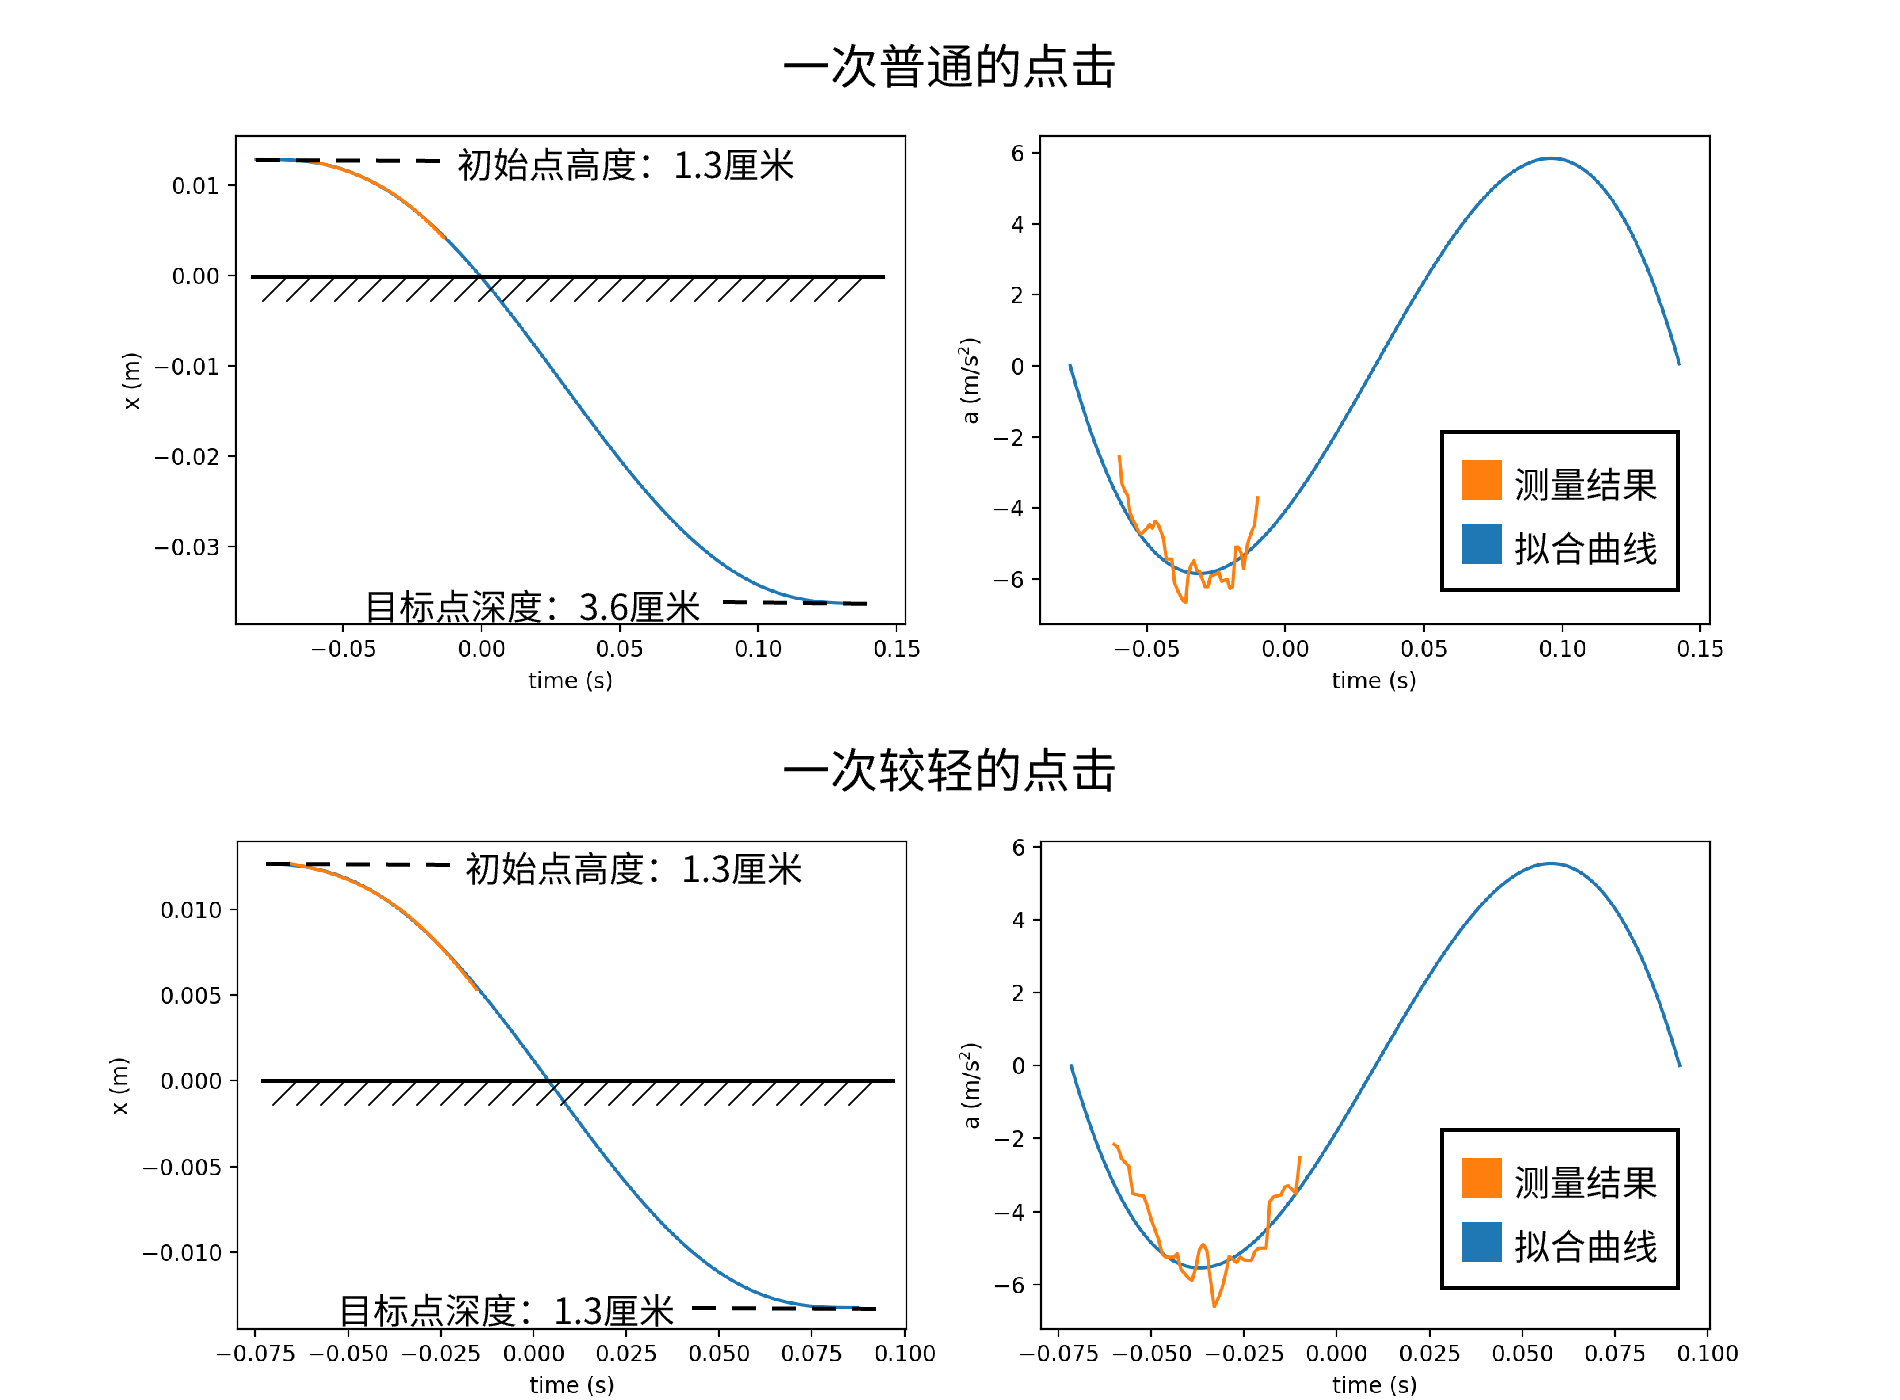
\includegraphics[width=0.8\linewidth]{model_fitting.png}
	\caption*{介绍}
	\caption{触摸运动计算模型的拟合实例}
	\label{fig:model_fitting}
\end{figure}

如上图所示是使用触摸运动计算模型拟合实际测量数据的两个实例,上方的两幅子图展示了一次普通力度点击的拟合效果,左上方是对触摸运动位移的拟合,右上方是对运动的加速度的拟合;下方的两幅子图展示了一次较轻点击的拟合效果。通过观察上图,读者很容易从中找到有用的信息,可用户指导触摸交互技术的改进。

\section{触摸运动的应用}

\textbf{(1)低延迟的触摸感知技术}:当实际测量结果与运动方程差异过大时,大到必定是外力作用(而不是手指运动或传感器误差时),可以判定为触摸事件的发生。

\textbf{(2)推测点击力度}:根据公式,可以精准计算触摸瞬间手指的速度,该速度与点击力度成正比。点击力度可用于拓展触摸交互的可达性[xx]。

\textbf{(3)为传感器的性能改进提供了指导}:例如,传感器的精度作用是平方级的,而传感器采样率的作用是线性的。

\textbf{(4)防误触技术}:在十指打字等连续触摸任务中,若对每只手指下落的过程拟合其运动方程,手指间运动方程的相关性是判断触摸意图的有力特征子。







\iffalse

其中,$\tau=\frac{t}{t_1-t_0}$表示当前时刻的运动进度。从公式中可以看出,无约束端到端运动在空间上沿直线运行,只在时间上存在一个先加速后减速的过程。

通过实验观察,我们发现了两种触摸运动,分别是:(1)长时触摸运动,即长按、拖拽等触摸过后手指保持与交互表面接触的触摸运动;(2)短时触摸运动,即轻敲、文本输入点击等触摸过后手指立即抬起的触摸运动。我们借鉴Tamar的手部运动模型[xx]来描述触摸运动,由于手部运动方程在笛卡尔坐标系的三个轴上的方程是独立的,且触摸运动的主要分量是手指与交互表面的距离$x$,以下我们仅研究$x$与时间$t$的关系:

\emph{“长时触摸运动:假设交互表面在触摸瞬间消失,长时触摸运动可描述为无约束端到端运动,其中起始点$x_0$是人产生触摸意图时手指的位置,手指将下落至位于交互表面之下的虚构目标点$x_1$,然后静止。”}

\emph{“短时触摸运动:假设交互表面在触摸瞬间消失,短时触摸运动可描述为过特定点的端到端运动,其中起始点$x_0$是人产生触摸意图时手指的位置,手指将下落至位于交互表面之下的虚构点$x_1$,随即抬起到目标点$x_2$。”}

【图:交互表面在触摸瞬间消失的情况】

对于无约束端到端运动,我们有$x^{'}(t_1)=0,x^{''}(t_1)=0$;对于上述过特定点的端到端运动,由于$x_1$是运动的最低点,手指下落经过$x_1$后立即上抬,因此手指在$x_1$点上的速度为零,且加速度大于零,即$x^{'}(t_1)=0,x^{''}(t_1)>0$。从公式可以看出,无论是长时触摸运动,还是短时触摸运动,其初始点$x_0$至虚构点$x_1$之间的运动方程都可以描述为:

\begin{equation}
	\begin{cases}
		x(t) \\
		s.t. x(0)=x_0,x^{'}(0)=x^{''}(0)=0,x(t_1)=x_1,x^{'}(t_1)=0,x^{''}(t_1)\geq0 \\
		min\frac{1}{2}\int_{0}^{t_1}\left(\frac{d^3x}{dt^3}\right)^2 dt
	\end{cases}
\end{equation}

但由于交互表面的存在,手指总是会在叨叨虚构点$x_1$之前被交互表面阻挡,瞬间停止,因此,只有起始点$x_0$到虚构点$x_1$之间

\subsection{过特定点的端到端运动}

与端到端的直线运动不同,现实生活中更多的手部运动沿弧线运行,根据Tamar的理论,现实生活中大部分弧线手部运动属于过特定点的端到端运动,即由下述用户意图引导的手部运动:

\emph{“在规定时间$t_2$内,最平稳地将手部从初始点$(x_0, y_0, z_0)$移动到目标点$(x_2, y_2, z_2)$,且必须在中途经过特定点$(x_1, y_1, z_1)$。”}

其中,“最平稳地”指的仍然是最小化手部运动急动度的平方的积分(公式\ref{equ:objective_function}),因此求解无约束端到端运动的方程等价于以下最优化问题:

\begin{equation}
	\begin{cases}
		x(t),y(t),z(t),t_1 \\
		s.t. x(0)=x_0,x^{'}(0)=x^{''}(0)=0,x(t_1)=x_1,x(t_2)=x_2,x^{'}(t_2)=x^{''}(t_2)=0 \\
		y(0)=y_0,y^{'}(0)=y^{''}(0)=0,y(t_1)=y_1,y(t_2)=y2,y^{'}(t_2)=y^{''}(t_2)=0 \\
		z(0)=x_0,z^{'}(0)=x^{''}(0)=0,z(t_1)=z_1,z(t_2)=z2,z^{'}(t_2)=z^{''}(t_2)=0 \\
		min\frac{1}{2}\int_{0}^{t_2}\left(\left(\frac{d^3x}{dt^3}\right)^2+\left(\frac{d^3y}{dt^3}\right)^2+\left(\frac{d^3z}{dt^3}\right)^2\right)dt
	\end{cases}
\end{equation}

上述最优化问题的解是:

\begin{equation}
	\begin{cases}
		x^{-}(\tau)=\frac{t_2^5}{720}(\pi_1(\tau_1^4(15\tau^4-30\tau^3)+\tau_1^3(80\tau^3-30\tau^4)-60\tau^3\tau_1^2+30\tau^4\tau_1-6\tau^5) \\ +c_1(15\tau^4-10\tau^3-6\tau^5))+x_0 \\
		x^{+}(\tau)=\frac{t_2^5}{720}(\pi_1(\tau_1^4(15\tau^4-30\tau^3+30\tau-15)+\tau_1^3(80\tau^3-30\tau^4-60\tau^2+10) \\ +c_1(15\tau^4-10\tau^3-6\tau^5+1))+x_2
	\end{cases}
\end{equation}

其中,$\tau=\frac{t}{t_2-t_0}$表示当前时刻的运动进度,$x^{-}(\tau)$是手部在经过特定点$(x_1, y_1, z_1)$之前(即$t<=t_1$)的运动方程,$x^{+}(\tau)$是手部在经过特定点$(x_1, y_1, z_1)$之后(即$t>t_1$)的运动方程。$t_1$的值可以通过动态优化问题[xx]求解。$\pi_1$和$c_1$是常数使得$x^{-}(\tau_1)=x^{+}(\tau_1)=x_1$。运动在y轴、z轴上的运动方程$y^{-}(\tau)$、$y^{+}(\tau)$、$z^{-}(\tau)$、$z^{+}(\tau)$与上述公式类似,且运动在三个轴上的方程相互独立。

\fi


% !TeX root = ../thuthesis-example.tex

\chapter{指环上的高准确低延迟触摸检测技术}\label{section:TappingRing}

\section{引言}

头戴式混合现实设备(MR头盔,如微软的Hololens\cite{hololens2})为新一代人机交互范式带来了丰富的可能性。MR头盔通过前置深度摄像头感知物理环境和用户动作,通过带有显示器护目镜将三维虚拟元素渲染在物理实体之上,原则上使得MR头盔用户可以随时随地与数字世界交互。MR头盔上一种也有前景、有价值的应用场景是在无源表面(如桌面、墙面)上投射虚拟用户界面,并允许人通过触摸与用户界面进行交互。上述应用场景将触摸交互——当前用户规模最大的人机交互方式,从有源触摸屏的束缚中解放出来,拓展到任意物理表面上。与目前MR头盔上流行的空中手势交互相比,触摸交互提供真实的触觉反馈,这是自然人机交互体验的重要组成部分。

要在MR头盔情境下检测无源表面的触摸交互,一个直观的想法是利用MR头盔的前置深度摄像头,通过视觉方法检测触摸事件。然而,视觉方法在检测触摸交互时存在固有的缺陷:首先,由于摄像头在手背的方向,摄像头在捕捉手指接触交互表面时面临严重的遮挡问题,在大多数情况下,摄像头都无法直接观察到手指接触交互表面的位置;第二,目前主流的深度摄像头是基于双目视觉的,这一类型的深度摄像头在识别交互表面的深度时精度不高,特别是当交互表面是纯色的、无明显视觉关键点的时候,误差可能达到厘米级别,对触摸交互技术的响应性带来很大挑战;第三,视觉方法的计算过程复杂,在计算资源有限的机器上运算可能会带来用户难以接受的延迟。例如,在利用视觉方法检测无源表面触摸交互的代表性工作MRTouch\cite{xiao2018mrtouch}中,研究者利用Hololens混合现实头盔的前置摄像头检测触摸事件,其未识别率高达3.5\%,误触率高达19.0\%,端到端延迟高达180 毫秒。这说明,基于视觉方法的无源表面触摸交互技术仍需改进。

\begin{figure}
	\centering
	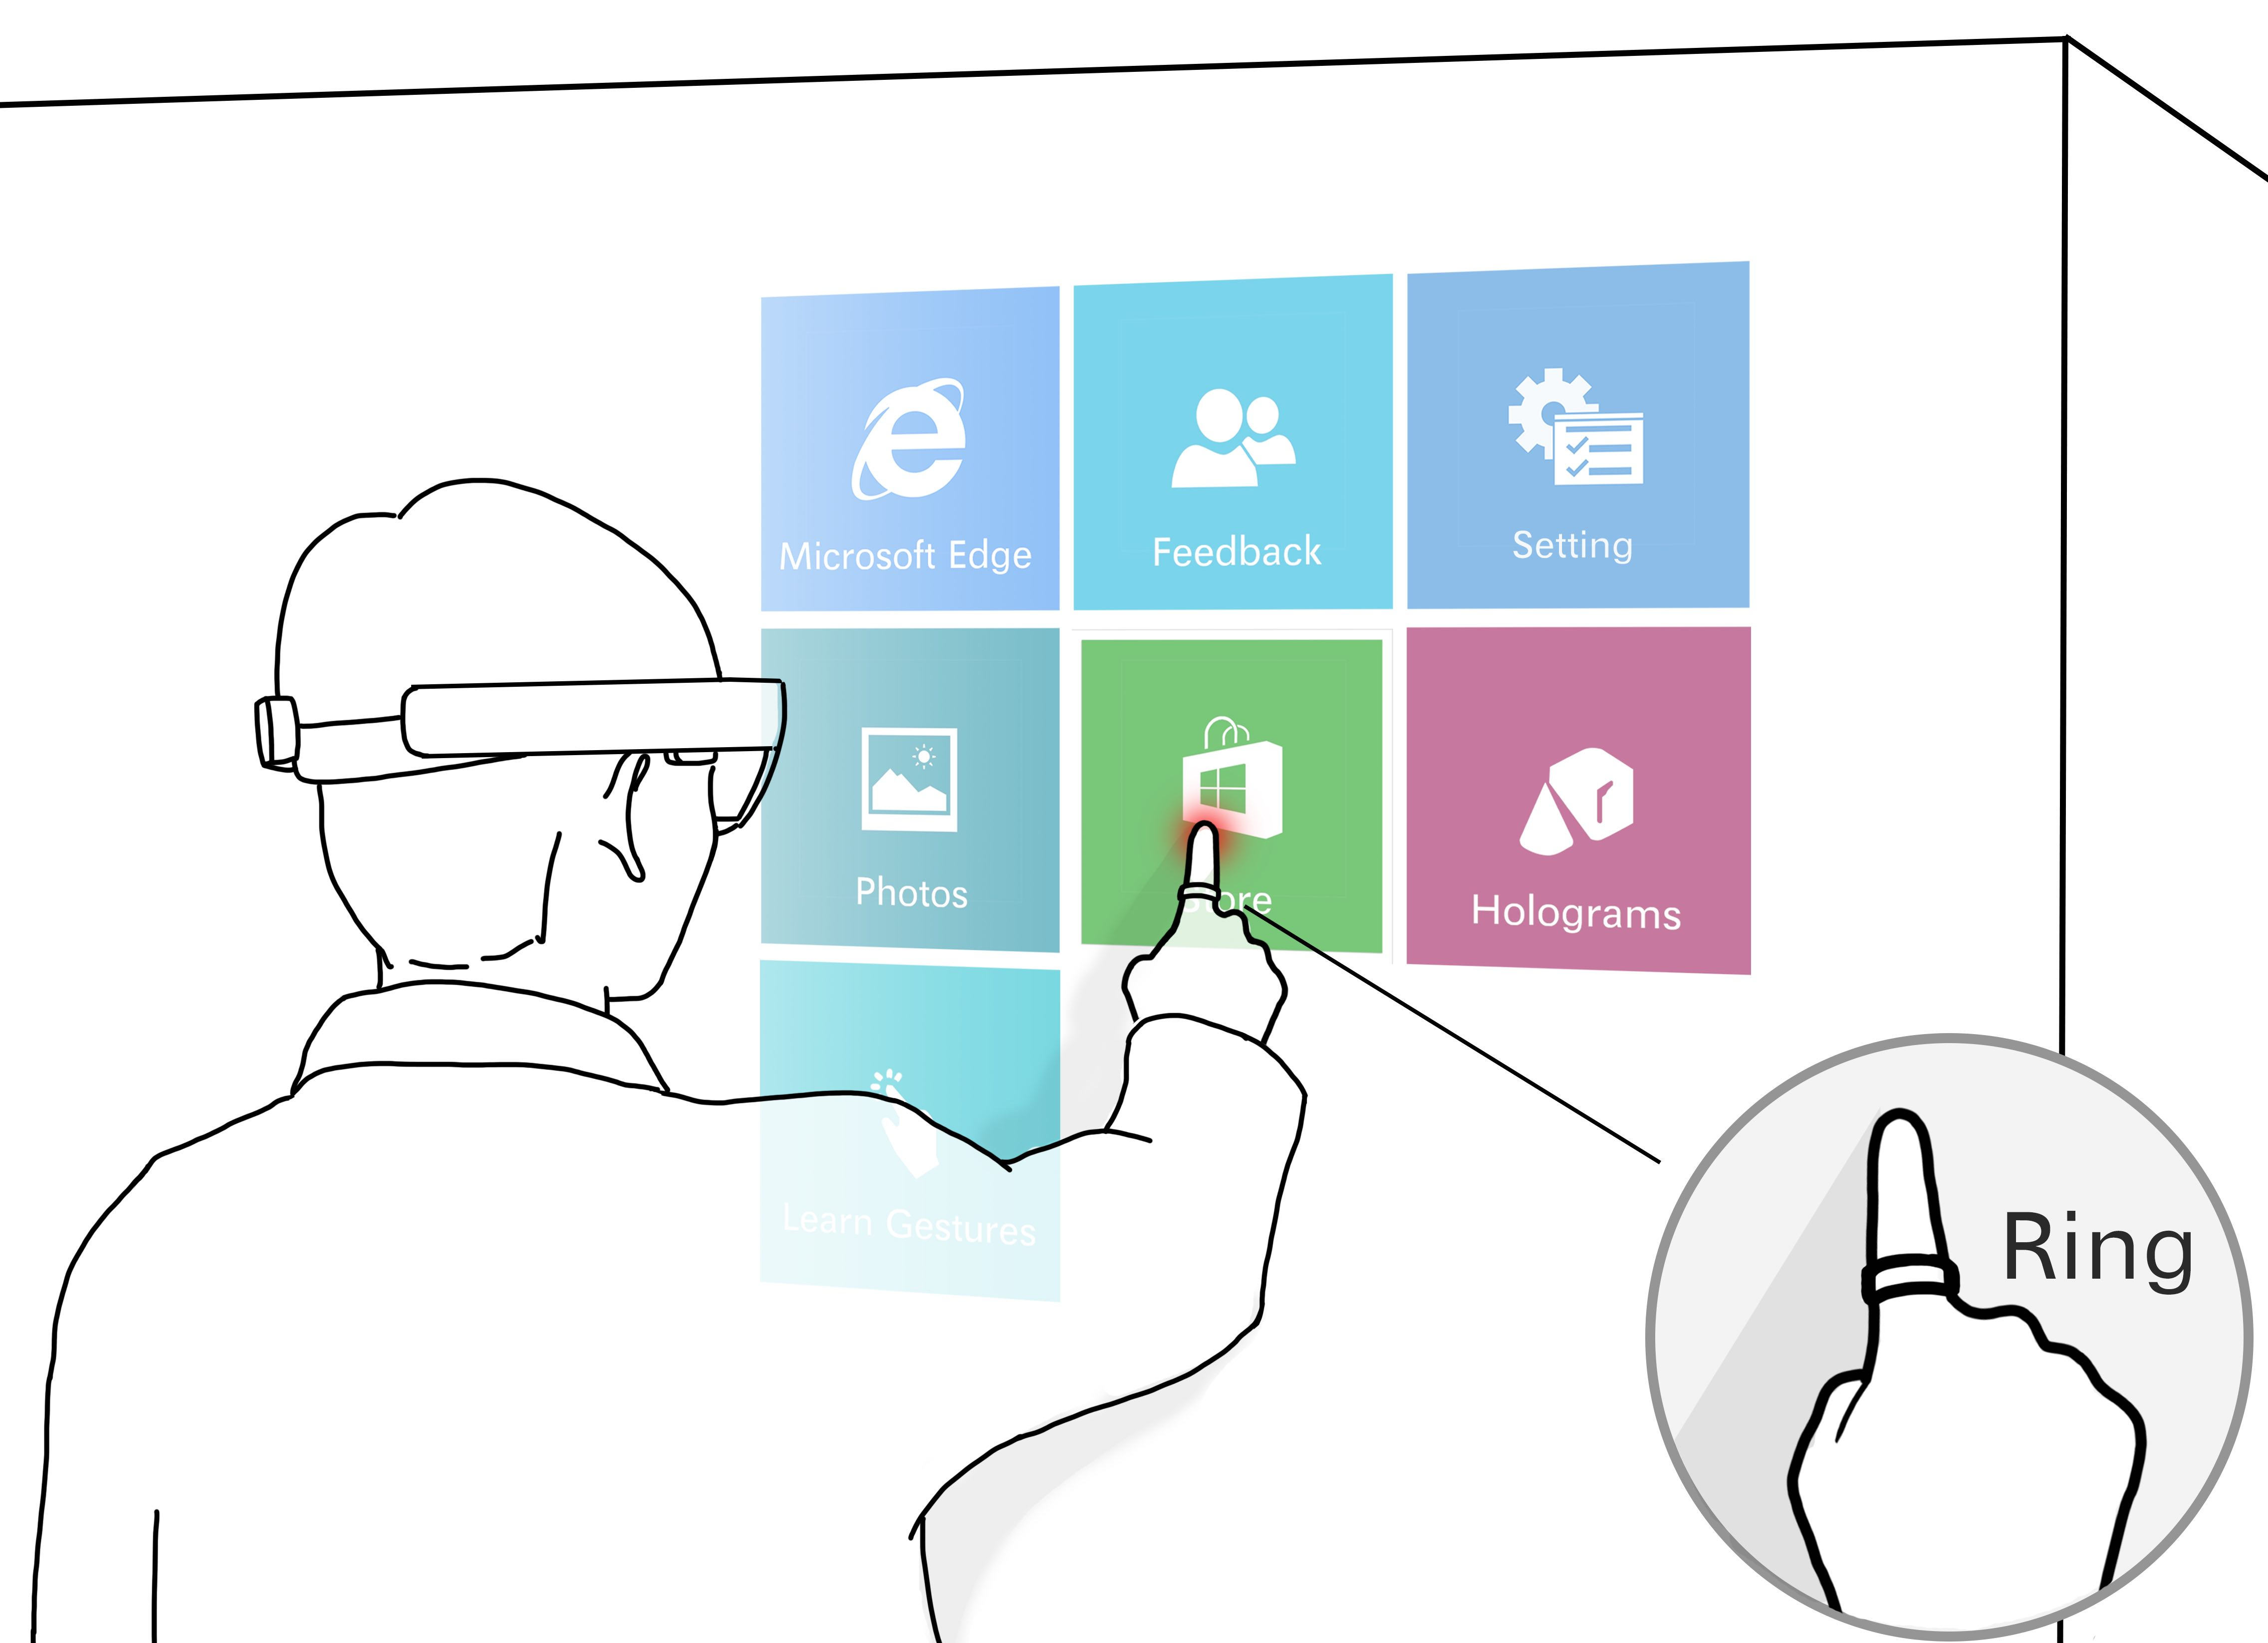
\includegraphics[width=0.8\linewidth]{MR_touch_envision.jpg}
	\caption*{结合MR头盔和智能指环有望在无源表面上支持流畅的触摸交互体验。}
	\caption{MR场景下触摸交互无处不在的设想}
	\label{fig:MR_touch_envision2}
\end{figure}

如图\ref{fig:MR_touch_envision2}所示,我们设想在未来结合MR头盔和智能指环来使能无源表面上流畅的触摸交互体验:MR头盔的前置摄像头主要负责识别手指的2D位置和姿态,而戴在手指上的惯性传感指环主要负责低延迟地检测手指是否接触到了交互表面。由于惯性传感器所提供的数据带宽较低,处理惯性传感器数据的计算通常是高效的,这确保了触摸检测的高响应性。在相关文献中,先前的工作已经探索过使用手指上佩戴的惯性传感器来增强触摸交互技术\cite{lam2002mids, oh2017anywheretouch, masson2017whichfingers}。使用智能指环感知触摸并不是本文的创新点,然而,先前工作仅对惯性传感器信号使用阈值方法来检测触摸事件,其响应性非常低下(准确率不超过89.8\%,延迟不低于50毫秒),因此基于惯性传感指环的触摸交互技术还有很大的改进空间。

为提高指环触摸交互技术的可用性,本文提出了基于惯性传感指环的低延迟触摸检测技术。低延迟是该技术与先前工作的主要区别,该技术的检测延迟低至10毫秒,而人无法在触摸交互中察觉到10毫秒的延迟,因此该技术在响应性上提供了最佳的用户体验。本章将从各个维度介绍基于惯性传感指环的低延迟触摸检测技术:

首先,本章开展了两项用户实验来调研触摸交互指环的设计问题,分别是用户对不同触摸姿态的主观喜好程度调研(实验一A),和用户对不同指环佩戴位置的主观喜好程度调研(实验一B),这两项实验的结果将指导技术的交互设计。然后,本章通过用户实验采集用户佩戴智能指环进行触摸交互的数据(实验二),再利用简单的机器学习方法实现了初版的触摸检测技术,用于对比指环佩戴在不同位置上时触摸交互技术的性能。最后,本章将触摸运动模型应用在指环触摸交互技术的改进上,介绍了基于基于惯性传感指环的低延迟触摸检测技术。评测实验(实验三)的结果显示,该技术的触摸检测准确率高达98.61\%(精确度98.61\%,召回率98.62\%),检测延迟低至10毫秒。这一结果说明,基于惯性传感指环的低延迟触摸检测技术具有高响应性,同时,该技术因支持无源表面触摸交互而具有高普适性,是一项有着广阔应用前景的新技术。

\section{相关工作}

本文引言已经提到,触摸交互技术主要分为有源触摸屏技术和无源表面触摸技术两大类。有源触摸屏技术是目前最常用的触摸交互技术\cite{lee1985multi, wang2009empirical, wilson2004touchlight},但由于它被束缚在有源表面上的内禀缺陷,触摸屏技术始终不具备适应未来穿戴计算交互模态的普适性。在MR头盔等新型交互设备兴起的背景之下,无源表面触摸交互技术是有前景的研究方向。无源表面触摸交互主要有种技术实现方案,基于摄像头的视觉方法和基于震动的方法,这两种方法在本质上分别对应触摸运动的位移信号和加速度信号。

\subsection{基于视觉的无源表面触摸交互}

摄像头可以通过视觉方法观察手指触碰交互表面的时间和位置,从而检测触摸事件,支持触摸交互。当摄像头部署在场景空间中,或作为可穿戴设备部署在人身上\cite{harrison2011omnitouch, xiao2018mrtouch},而非直接部署在交互表面上时,即可认为摄像头支持无源表面上的触摸交互,具有较高的普适性。在相关工作中,已有研究者利用激光雷达\cite{paradiso2000sensor}、RGB摄像头\cite{agarwal2007high, chang2005real, letessier2004visual, sugita2008touch}、红外摄像头\cite{grudin2001integrating}、热成像摄像头\cite{saba2012dante}和深度摄像头\cite{agarwal2007high, xiao2016direct, xiao2018mrtouch, benko2012miragetable, harrison2011omnitouch, wilson2010combining}实现基于视觉方法的无源表面触摸交互技术。然而,先前基于视觉的触摸交互技术的基本原理都是直接观察手指是否接触交互表面,这种方法面临严重的遮挡问题,影响了触摸交互技术的响应性,即使在最新工作中\cite{xiao2018mrtouch},该方案的误触率也高达19.0\%,端到端延迟高达180毫秒。本文的触摸运动模型为基于视觉的无源表面触摸交互技术带来了新思路,不同于先前技术中摄像头“直接”观察手指是否触摸表面的思路,触摸运动模型揭示:可以通过手指触摸表面时的瞬停现象“间接”地判断触摸事件,从而有效规避遮挡问题,提高触摸检测的响应性。

\subsection{基于震动的无源表面触摸交互}

在触摸交互中,当手指接触到交互表面上时,会引发手指的震动,并且发出声音。震动和声音可以被惯性传感器和麦克风所捕捉,因此,不少工作致力于探索基于震动的无源表面触摸交互,利用部署在人的手指\cite{gu2019accurate, shi2020ready, gu2020qwertyring}或手腕\cite{meier2021tapld}上的传感器感知触摸。然而,先前工作仅通过阈值方法感知触摸\cite{lam2002mids, oh2017anywheretouch, niikura2014anywhere},即当手指震动幅度或声音响度超过特定阈值时判定触摸发生,其准确率不超过89.8\%,端到端延迟不低于50毫秒,不满足触摸交互的高响应性需求。本文的触摸运动模型为基于震动的无源表面触摸交互技术提供计算理论基础,模型指出,除去手指接触交互表面瞬间引发的震动以外,手指向下过程中的众多运动信号规律都有助于提高触摸检测技术的响应性。在触摸运动模型的基础之上,本文作者在2019年提出基于惯性传感指环的低延迟触摸检测技术\cite{gu2019accurate},亦即本章所介绍的内容,该技术将无源表面触摸交互技术的响应性提升到用户无法察觉到延迟的标准,后来有研究者跟随并改进了这份工作。例如,本文作者和Shi等人在同一时期提出惯性传感指环不仅可用户检测单次触摸事件,还可以识别长按、滑动拖拽等触摸手势\cite{gu2020qwertyring, shi2020ready};Meier等人提出通过两个惯性传感器,可以将设备从手指上转移到手腕上\cite{meier2021tapld},而不会严重影响触摸交互技术的检测性能。

\subsection{触摸姿态}

触摸姿态指的是触摸交互中,人的手指接触交互表面时的全手型姿态,例如,食指指腹点击、中指指尖敲击、食指第二关节叩击、三指触摸都是不同的触摸姿态。触摸交互技术若能区分不同的触摸姿态,将能丰富触摸交互的表达力\cite{cao2008shapetouch, harrison2011tapsense},然而因为目前主流的触摸屏技术无法区分不同的触摸姿态,所以相关研究一直停留在实验室阶段。随着触摸交互技术的发展,触摸姿态的多样化将被相关技术所支撑,这也是本章将就用户对不同触摸姿态的主观喜好程度进行实验调研的动机。除了触摸姿态以外,触摸压力\cite{ramos2004pressure}、速度\cite{heo2011forcetap, iwasaki2009expressive}、切向力\cite{heo2011force}和手指朝向\cite{roudaut2009microrolls, xiao2015estimating}等额外的输入信道也能丰富触摸交互的表达力,可作为未来的研究方向。

\section{指环触摸交互的自然性研究}

由于指环上无源表面触摸交互技术对普通用户而言是陌生的,本章重视该交互方式的自然性研究。为此,本章开展了两项用户实验来探索指环触摸交互的自然性问题,分别调研了用户对不同触摸姿态和不同指环佩戴位置的主观喜好程度,从而指导本智能指环触摸检测技术的交互设计。

\subsection{实验一A:触摸姿态主观喜好程度调研}

本着人机交互以人为中心的原则,好的触摸交互技术应支持用户喜好的触摸姿态,而非易于识别的触摸姿态。为此,实验一A通过实验和问卷调研被试对不同触摸姿态的喜好程度,以寻找触摸交互技术应支持的触摸姿态集合。首先,我们定义了一套触摸姿态全集;然后,对于触摸姿态全集中的每个姿态,我们要求被试分别将水平的桌面和垂直的墙面视为交互表面,使用该姿态进行“触摸”,亲身感受后在问卷中对该触摸姿态进行评分。最后,实验者根据被试的评分选择出最受用户喜好的触摸姿态集合。

\subsubsection{触摸姿态全集}

如图\ref{fig:posture_set}所示,我们通过一个三维的设计空间来探索触摸姿态的全集,这三个维度分别是:

\begin{itemize}
\item \textbf{哪些手指触摸交互表面?}选项包括拇指、食指、中指、无名指、小指、双指和三指。
\item \textbf{手指的哪个部分触摸交互表面?}参考相关工作TapSense\cite{harrison2011tapsense},选项包括指腹、指尖、手指第二关节、指侧和指甲。
\item \textbf{手部状态?}选项包括五指张开和握拳。
\end{itemize}

\begin{figure}
	\centering
	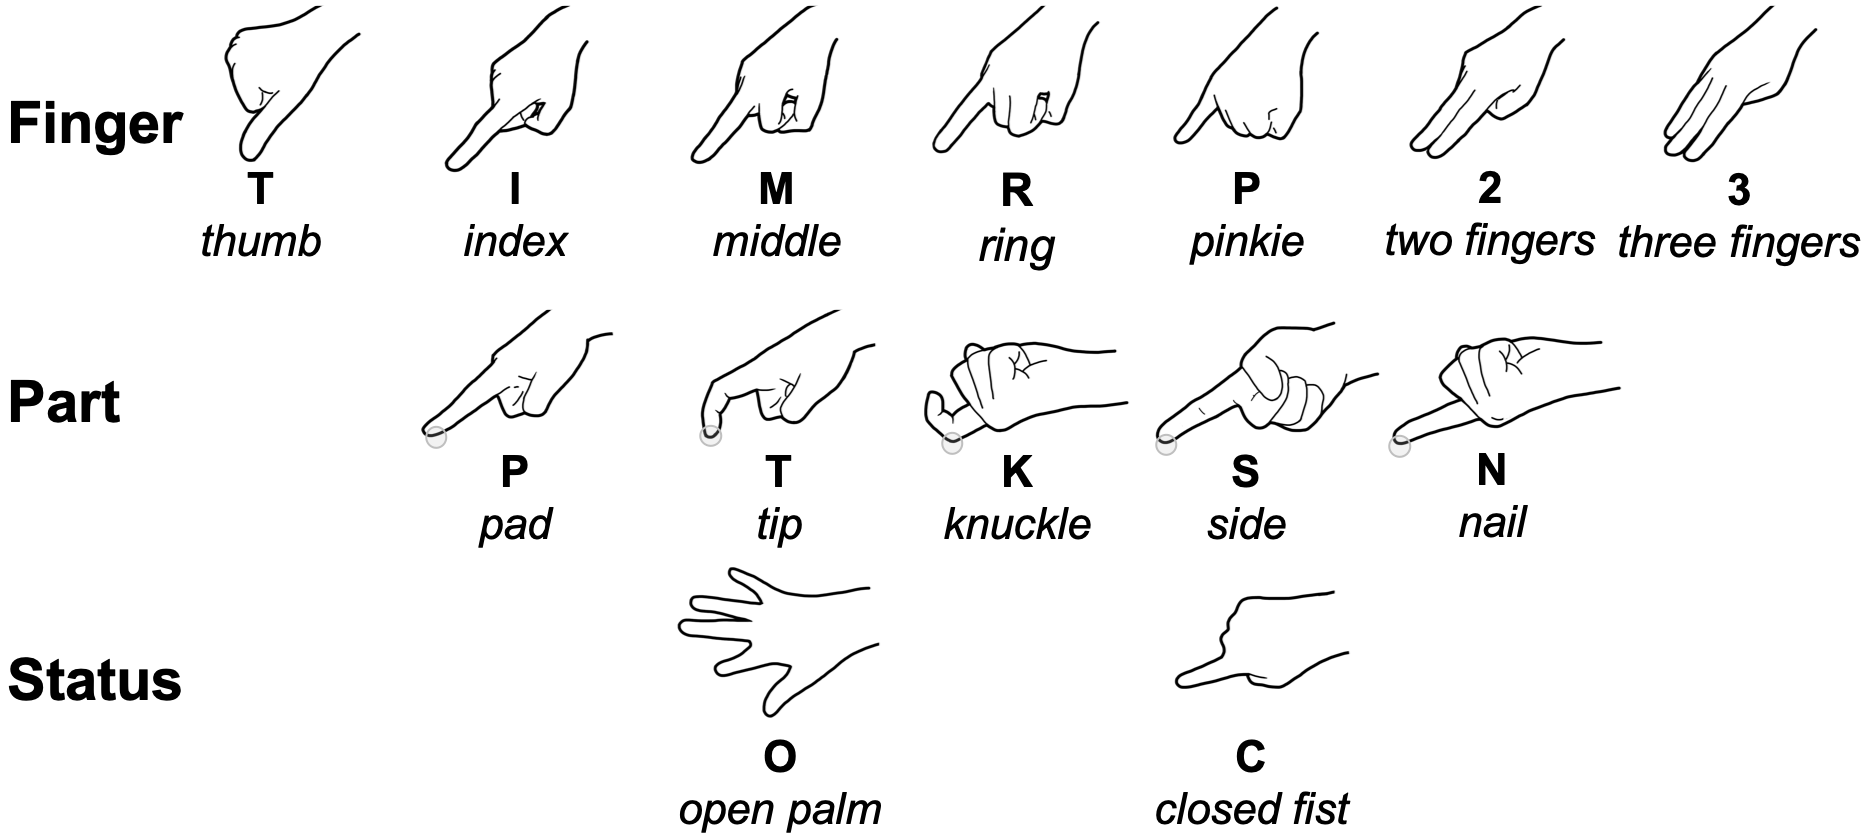
\includegraphics[width=0.8\linewidth]{posture_set.png}
	\caption*{触摸姿态的设计空间有三个维度,分别是哪些手指触摸、手指的哪个部分触摸和手部状态,三个维度的笛卡尔积就是触摸姿态全集。其中,粗体字母是根据每个状态的英文描述起的缩写。}
	\caption{触摸姿态的三维设计空间}
	\label{fig:posture_set}
\end{figure}

以上设计空间中三个维度的笛卡尔积即为触摸姿态的全集,共包含$7\times5\times2=70$种触摸姿态。实验者为他们定义了缩写,例如,五指张开状态下食指指腹触摸的缩写为IPO,其中I对于食指,P对应指腹,O对应五指张开的状态。

\subsubsection{实验设计和过程}

实验者从校园中招募了20名被试,其中7名为女性,被试的年龄是18岁到27岁不等,平均年龄为22.0岁。实验在两种交互表面上开展,分别是水平的桌面和垂直的墙面,它们是日常生活中场景的物体表面。实验采用组内实验设计,实验者采用拉丁方平衡被试在两种不同交互表面上的实验顺序。由于触摸姿态全集包含70中触摸姿态,而实验在两种交互表面上开展,每位被试在$70\times2=140$种设置下体验触摸交互,并给出评分。实验问卷采用了七级李克特量表,在三个方面上收集用户对每种触摸姿态的评分:

\begin{itemize}
\item \textbf{舒适度}:以该姿态触摸的物理和心理轻松程度(1 - 不轻松,7 - 非常轻松)。
\item \textbf{易记度}:记住该触摸姿态的难以程度(1 - 不容易,7 - 非常容易)。
\item \textbf{喜好度}:对该触摸姿态的总体喜好程度(1 - 完全不喜欢,7 - 非常喜欢)。
\end{itemize}

在实验的最后,实验者针对以下问题对被试进行了简短的采访:(1)您认为在本实验的触摸姿态全集之外是否有其它可用的触摸姿态?(2)在日常使用中,您愿意记住多少种不同的触摸姿态?

实验中,被试坐在可调节的椅子上,在开始实验前,被试需要调整座椅,让自己以最舒适的姿态进行接下来的实验。对于每一个触摸姿态,实验者都会首先进行示范,然后被试亲自执行该触摸姿态三遍,然后在问卷中对该触摸姿态的舒适度、易记度和喜好度评分。由于李克特量表的主要通过相对数值对比不同的被测量值,每一次触摸之后,被试都可以通过对比来修改之前作出的评分。被试每执行十个触摸姿态,就需要休息五分钟的时间,以避免疲劳。整个实验耗时一个小时。

\subsubsection{实验结果}

\begin{figure}
	\centering
	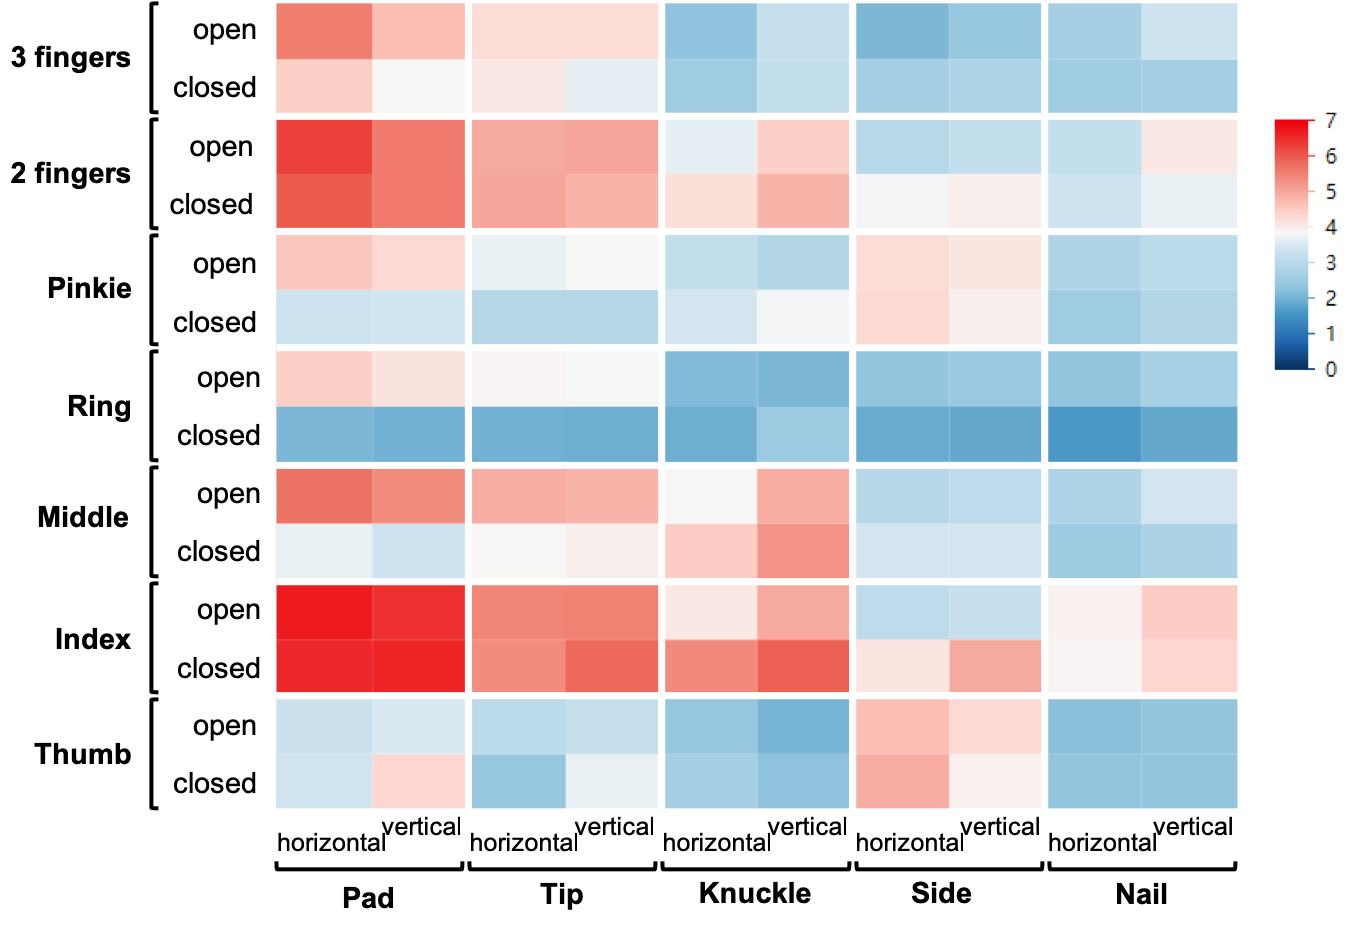
\includegraphics[width=0.8\linewidth]{posture_preference.png}
	\caption*{20名用户对两种交互表面上、70种不同触摸姿态的平均喜好程度,其中,1分表示完全不喜欢,7分表示非常喜欢。}
	\caption{触摸姿态主观评分热力图}
	\label{fig:posture_preference}
\end{figure}

图\ref{fig:posture_preference}展示了被试在水平和垂直交互表面下对所有70种触摸姿态的喜好程度评分,图\ref{fig:posture_top10}展示了被试们最喜好的触摸姿态前十名。Friedman检验显示交互表面的水平和垂直与否并不显著影响用户对各触摸姿态的喜好。在实验后的采访中,没有任何被试报告在触摸姿态全集以外存在其它可用的触摸姿态,因此,实验者认为图\ref{fig:posture_top10}中的就是人们最喜好的十种触摸姿态。

\begin{figure}
	\centering
	
\includegraphics[width=0.8\linewidth]{posture_top10.png}
	\caption*{在人们最喜好的十种触摸姿态中,有七种姿态来自常用的单指或多指指腹点击,另有ITO(食指指尖敲击-张手)、ITC(食指指尖敲击-握拳)和IKC(食指第二关节叩击-握拳)。}
	\caption{人们最喜好的触摸姿态前十名}
	\label{fig:posture_top10}
\end{figure}

喜好程度排名前五的触摸姿态分别是IPO(食指指腹触摸-张手)、IPC(食指指腹触摸-握拳)、2PO(双指指腹触摸-张手)、2PC(双指指腹触摸-握拳)和ITO(食指指尖敲击-张手),这些姿态都是目前常用的触摸手势。喜好程度排六到十名的触摸姿态是ITC、MPO、IKC、2TO和3PO,其中MPO(中指指腹触摸-张手)和IKC(食指第二关节叩击-握拳)值得关注:若触摸交互技术有能力区分食指指腹触摸和中指指腹触摸,部分用户将愿意让中指触摸表达特定的交互语义;食指第二关节叩击是触摸屏上不常用的触摸姿态,但近年来被华为手机用于触发截屏功能,从本实验结果来看,这一交互方式应会广受用户好评。

Friedman检验显示,“哪些手指触摸交互表面”($\chi^2=767.70, p<.0001$)和“手指的哪个部分触摸交互表面”($\chi^2=423.86, p<.0001$)都对被试的主观评分有显著性影响。被试更喜欢用食指、中指、两指和三指进行触摸交互,不喜欢用拇指、无名指和小指触摸。被试只接受指腹点击、指尖敲击和手指第二关节叩击,厌恶手指侧面点击和手指甲敲击。在实验后的采访中,被试报告说他们平均愿意记住 7.45(SD=2.61)个触摸姿态,这是因为,如果交互系统中表达特定交互意图的手势太多,会给用户带来很大的认知负担。因此,实验者认为这十种最受欢迎的触摸姿态是值得进一步研究的,也值得本章的低延迟触摸检测技术去检测,而这十种触摸姿态以外的情形就不需要更多的关注了。

\subsection{实验一B:指环佩戴位置主观喜好程度调研}

本小节介绍一个简短的用户实验,实验目的是调研用户对指环佩戴位置的主观喜好程度,其中,指环是用于触摸交互的智能指环,而非用于装饰的戒指。如图\ref{fig:ring_positions}(a)所示是实验所评测的九种不同的指环佩戴位置,分别是食指、中指和无名指的第一、二、三指骨。实验中,被试需要将一个嵌入了惯性传感器的指环佩戴在手指的不同位置上,在桌面上以自己喜欢的姿态触摸若干次,然后通过问卷对其体验进行主观评分。问卷采用七级李克特量表(1分 - 最差,7分 - 最好),在三个方面上收集用户对指环佩戴位置的主观看法:

\begin{itemize}
	\item \textbf{舒适度}:在此位置上佩戴指环进行触摸交互的舒服程度。
	\item \textbf{接受度}:在此位置上佩戴指环的社会接受程度,比如,是否会吸引他人不必要的注意。
	\item \textbf{喜好度}:对该指环佩戴位置的总体喜好程度。
\end{itemize}

\begin{figure}
	\centering
	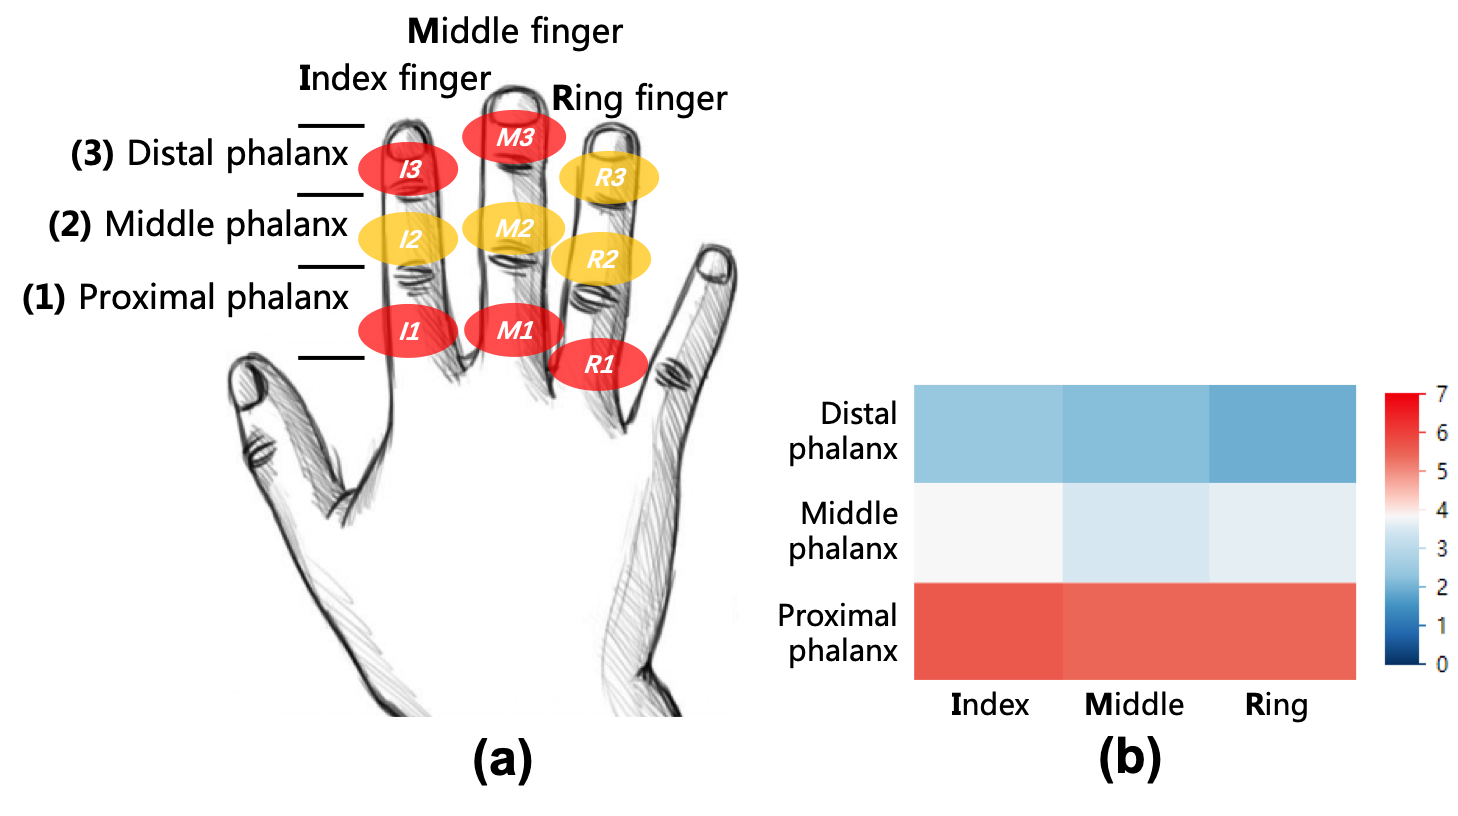
\includegraphics[width=0.8\linewidth]{ring_positions.png}
	\caption*{图a展示了实验所评测的九种不同的指环佩戴位置,实验者为每个位置定义了缩写,例如,I1表示食指的第一指骨;图b是被试对不同指环佩戴位置的喜好程度(1 - 完全不喜欢,7 - 非常喜欢)}
	\caption{指环佩戴位置主观评分热力图}
	\label{fig:ring_positions}
\end{figure}

实验一A的20名被试参与了本实验,如图\ref{fig:ring_positions}(b)所示,被试更喜欢在食指第一指骨(5.65分)、中指第一指骨(5.45分)和无名指第一指骨(5.45分)上佩戴指环,在这些指根的位置上佩戴指环是舒适、且可接受的。将指环佩戴在手指的第二指骨上的主观评分是中肯的,而将指环佩戴在手指末端令人厌恶。实验结果表明,人们更愿意将智能指环佩戴在手指的第一指骨上,但具体是戴在食指、中指还是无名指上都差异不大。因此,基于惯性传感指环的触摸检测技术应尽可能通过指根上的运动传感信号感知触摸事件。

\section{基于机器学习的触摸检测技术}

\subsection{实验二:收集触摸数据}

实验二采集了被试进行触摸交互的惯性传感器数据和头戴式摄像头数据,实验的动机是为两项后续工作提供数据支持:一是基于摄像头的触摸姿态识别,二是基于惯性传感信号的触摸检测技术。

\subsubsection{实验设计和过程}

实验者从校园中招募了12名学生作为被试,其中有4名女性,被试的年龄从20岁到29岁不等,平均年龄为23.1岁。实验分为两大部分,每名被试分别在水平的桌面和垂直的墙面上进行实验。实验采用了组内实验设计,实验者采用拉丁方平衡了水平或垂直表面的实验顺序。

对于每种交互表面,需要进行五段实验:如图\ref{fig:ring_positions}手指上的红色区域所示,每段实验中被试分别在五个不同的位置上佩戴智能指环,这五个位置分别是I1(食指第一指骨)、M1(中指第一指骨)、R1(无名指第一指骨)、I3(食指第三指骨)和M3(中指第三指骨)。选择I1、M1、R1等手指第一指骨位置是因为实验一的结果表明,用户更喜好将智能指环佩戴在这些位置上;而加入I3和M3这两个位置是因为实验者猜测,手指末端上惯性传感器所采样的触摸信号的震动强度更大,利用该信号感知触摸事件的能力可能会更强,实验者需要通过实验对比来验证此猜测是否成立。实验舍弃了采集指环佩戴在I2、M2、R2和R3位置上的触摸数据,这是因为冗余的、时间过长的实验可能会导致被试的疲劳,影响数据的可靠性。

每段实验包含十组,在每组实验中,被试分别以如图\ref{fig:posture_top10}所示的十种触摸姿态接触交互表面,各20次。实验者要求被试尽可能用自然的方式进行触摸交互,每名被试总共进行了$2\times5\times10\times20=2000$次触摸。最后,实验者还收集了一系列空中手势作为负样本,被试将惯性传感指环佩戴在不同的位置,执行画圈、画方框、空中点击等手势。采集空中手势的过程中,被试不允许让手指接触到其它物体。对于每个指环佩戴位置,需要采集持续一分钟的空中手势数据。在实验中,被试要在每200次触摸后休息两分钟,以避免疲劳问题。整个实验持续了一个半小时。

\subsubsection{实验设备}

如图\ref{fig:tapping_ring_config}所示是实验二的实验设置。被试在手指上佩戴了惯性传感指环,头上戴着一种商用手型追踪摄像头(LeapMotion),被试在一块自制的超低延迟触摸板上进行触摸交互。实验通过指环中的惯性传感单元采集加速度和角速度信号,通过LeapMotion采集手部的骨骼点数据,通过触摸板采集接触与否的真值。

\begin{figure}
	\centering
	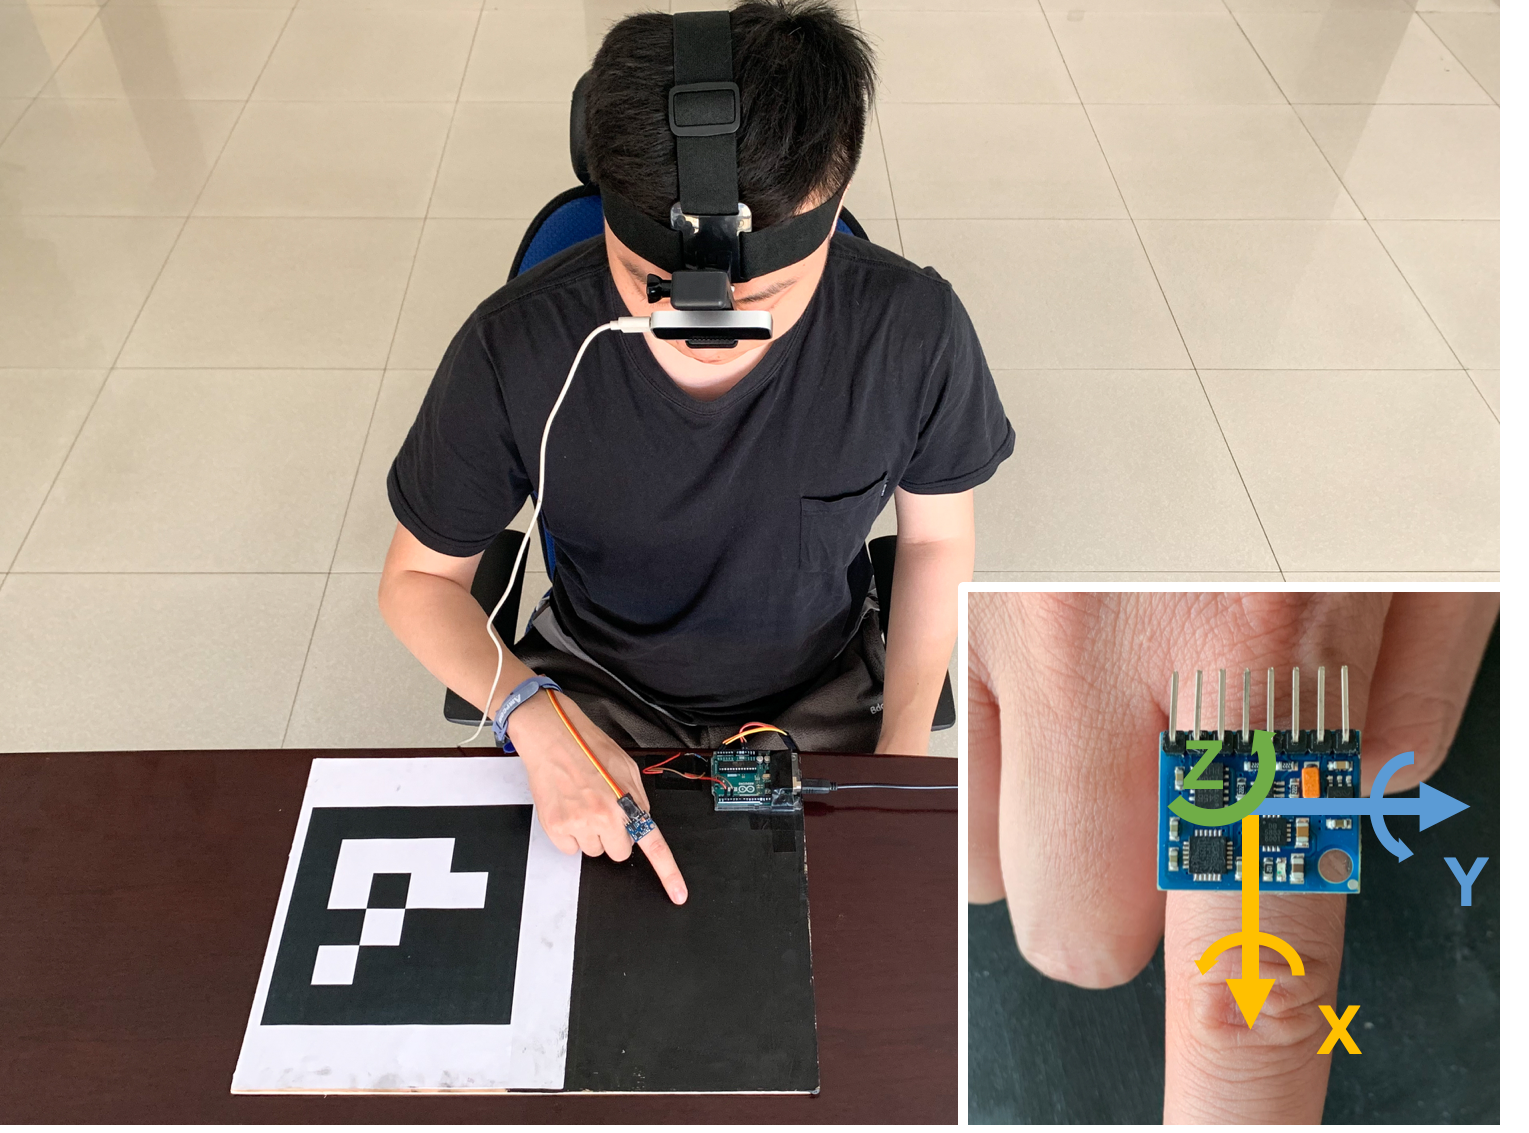
\includegraphics[width=0.6\linewidth]{tapping_ring_config.png}
	\caption*{实验二的实验设置,被试佩戴惯性传感指环接触触摸屏。子图展示了惯性传感指环及其信号所在的坐标系。}
	\caption{实验设置}
	\label{fig:tapping_ring_config}
\end{figure}

惯性传感指环由一个九轴的惯性传感单元(GY-85)和常规的戒指粘合而成,实验者一共制作了四个大小不一的惯性传感指环,以适应不同被试的手指大小,惯性传感单元通过杜邦线连接在Arduino(Uno R3)开发板上。实验者用魔术贴将杜邦线固定在被试的手腕上,以求在最大程度上减轻杜邦线对用户触摸交互造成的影响。超低延迟触摸板是一块覆盖有导电墨水的木板,当手指触摸到木板时,木板与用户的手指形成耦合电容,电容会增加,实验者利用这一现象来判断手指接触木板的精确时间\cite{badger2018capacitive}。

触摸板也通过杜邦线与Arduino连接,它和惯性传感指环共享相同的时间戳,他们的频率都为200赫兹。高速摄像头的图像分析表明,从人触摸木板到Arduino开发版上的信号灯亮起所需时间不超过5毫秒,也就是触摸板的延迟在5毫秒以下。触摸板旁边是一个二维码标识符,用于准确标记交互表面所在位置,以配合LeapMotion计算人的手指上每个关节与交互表面之间的距离。LeapMotion的传感频率为60赫兹,其与Arduino之间的传输延迟大概为20毫秒。LeapMotion在工作原理上依赖其自带的红外照明,一般而言,它时而会出现手型估计失败的情况,为此实验者非常注重实验的关照条件:实验在灯光明亮且避免阳光的环境中进行,触摸板上的导电墨水也专门采用吸收红外光的墨水,为摄像头提供了黑色背景,以上实验环境使得LeapMotion的传感精度得到保障。

\subsubsection{实验数据统计}

本实验共采集了$12\times2000=24000$次触摸的实验数据。实验者开发了一个交互式程序,用以人工剔除明显错误的数据,例如,有时候指甲太长的用户接触触摸板时,触摸板无法及时报告触摸事件。在剔除错误数据之后,实验共产生了超过23900 份有效的数据作为触摸的正样本,实验者从空中手势中随机抽取负样本,正样本和负样本的数量相同。

\subsection{基于机器学习的触摸姿态分类}

本小节将介绍基于支持向量机(SVM)的触摸姿态分类方法,该方法较为直观,其目的只是评测采用视觉方法分类触摸姿态的可行性,而非本文的贡献。若该方法的分类准确率达到可观的水平,说明本章提出的MR头盔加智能指环的组合不仅可以检测触摸事件,还能区分不同的触摸姿态。

\subsubsection{技术方案}

本小节参考了相关论文\cite{de2016skeleton}提取手部骨骼特征,特征包括手指尖与交互平面的距离、手指尖之间的距离、手指尖与手掌的距离和手指尖与手掌平面之间的夹角,这些值拼接成19维的手型特征向量,实验者根据此特征向量提取方法训练SVM模型,该模型即可分类不同的触摸姿态。

\subsubsection{评测结果}

如表\ref{tab:posture_accuracy}所示,实验者采用留一(被试)交叉验证法评估触摸姿态分类的准确率。IPO、IPC、2PC、IKC这四种最常用的触摸姿态的四分类准确率达到99.0\%,这说明触摸姿态四分类具有较高的可行性;在四分类的基础上,外加2PO、MPO 和 3PO这三种触摸姿态,得到七分类的准确率为88.5\%,这说明触摸姿态七分类的准确率仍在可接受范围内;然而,所有常用触摸姿态的十分类准确率却很不理想,准确率仅为77.0\%,这说明就目前的视觉技术而言,要准确分类十个或者以上的触摸姿态仍比较困难。

\begin{table}
	\centering
	\caption{触摸姿态分类的准确率(括号中数值为标准差)}
	\begin{tabular}{llll}
		\toprule
		无 & 四分类 & 七分类  & 十分类 \\
		\midrule
		水平桌面 & 99.1\% (1.3\%) & 89.5\% (3.9\%) & 76.4\% (6.8\%) \\
		垂直墙面 & 99.0\% (1.4\%) & 87.6\% (4.8\%) & 77.6\% (6.7\%) \\
		\bottomrule
	\end{tabular}
	\label{tab:posture_accuracy}
\end{table}

上述实验结果表明,头戴式前置摄像头大约可以稳健地区分四到七种不同的触摸姿态。随着手部跟踪技术的发展\cite{ge2018hand, spurr2018cross, yuan2018depth},作者认为,通过触摸姿态的多样化来丰富触摸交互将很快成为可能。

\subsection{基于机器学习的触摸检测技术}

本小节将介绍基于支持向量机(SVM)的触摸检测技术。支持向量机是一种简单的机器学习方法,具有开发敏捷的特点,因此,本小节的目的并不是实现终版触摸检测技术,而是通过简单的机器学习方法探索指环触摸检测技术中尚待确定的因素。

\subsubsection{数据分析}

惯性传感指环的中能收集到的数据包括指环的加速度、角速度和磁力计数据。由于磁力计数据的刷新频率只有8赫兹,实验者舍弃了磁力计数据。原始的加速度数据中混杂了重力,实验者通过Madgwick过滤器\cite{madgwick2010efficient}将原始加速度信号分解为加速度和重力。最后,经过处理的实验数据共包含九个维度,包括三轴加速度、三轴角速度和三轴重力。

\begin{figure}
	\centering
	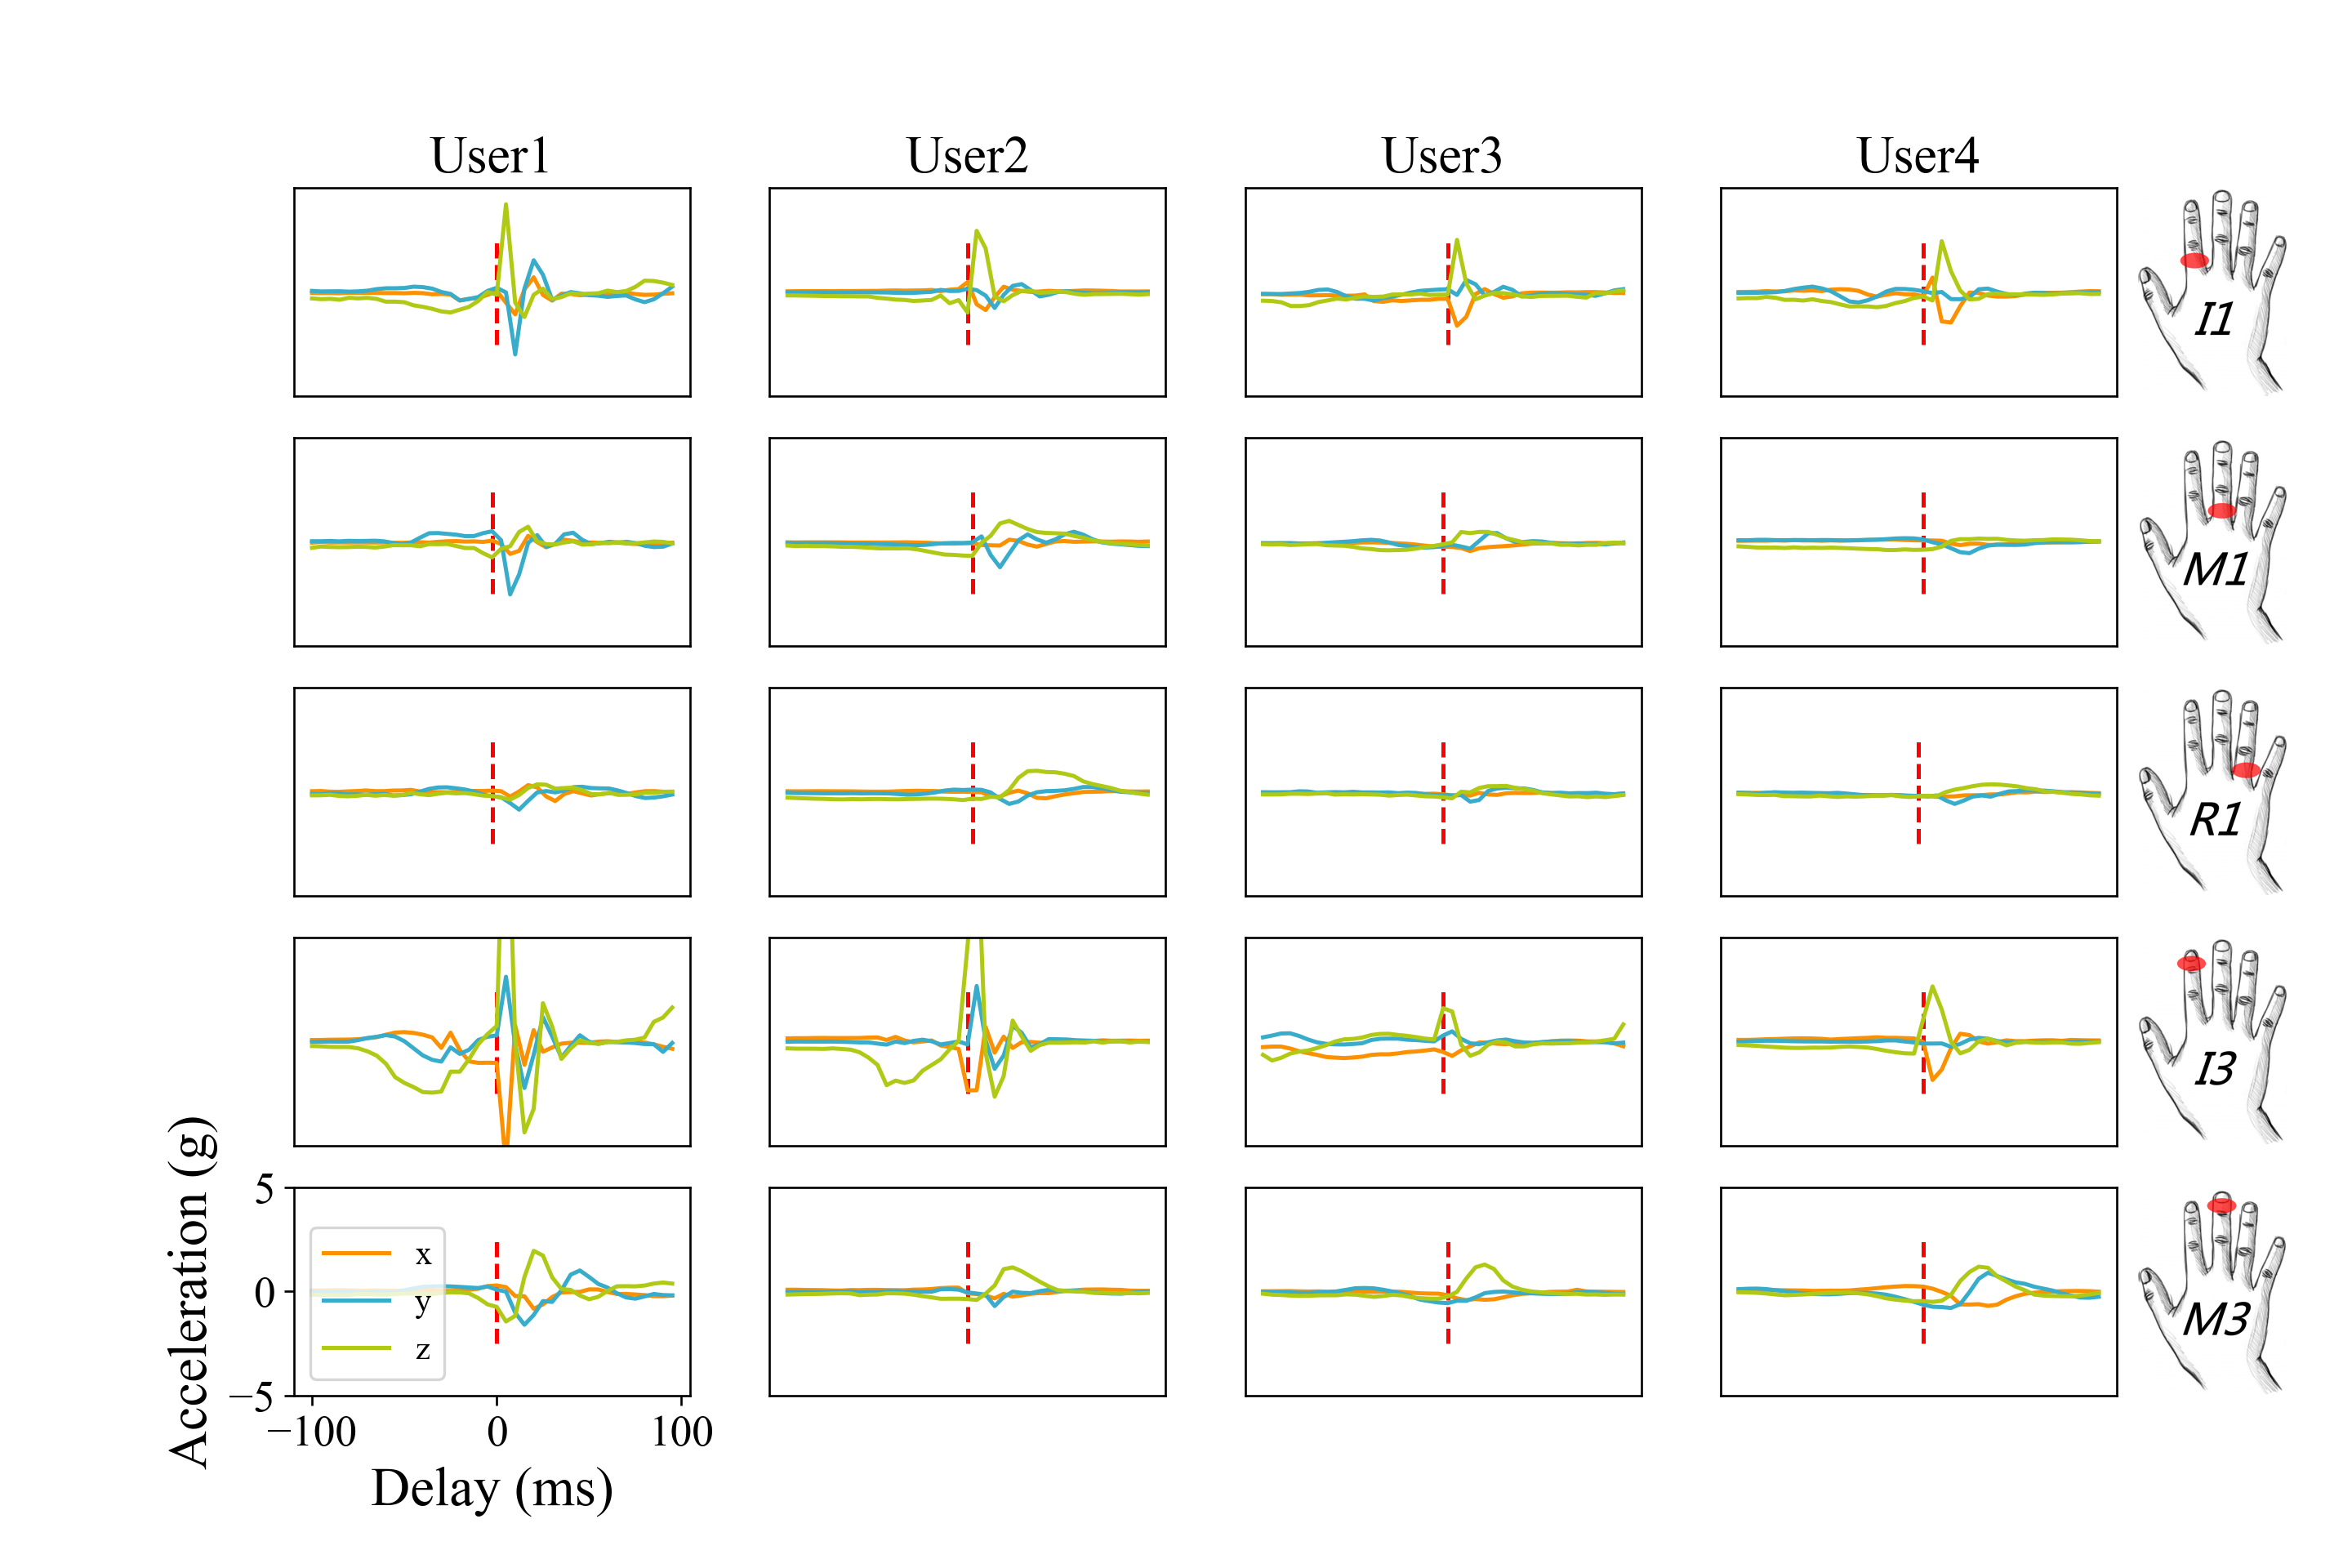
\includegraphics[width=0.8\linewidth]{IMU_acc_hands.png}
	\caption*{图中展示了被试执行食指指腹触摸时的惯性传感器加速度信号,四纵列子图对应四个不同的被试,五横列子图对应了五种不同的指环佩戴位置。}
	\caption{加速度信号图示}
	\label{fig:IMU_acc_hands}
\end{figure}

如图\ref{fig:IMU_acc_hands}所示,本小节以食指指腹点击这一触摸姿态为例分析数据规律。从图中可以看出,触摸导致的震动会传导到各个手指的各个位置上,形成一个幅度较大、较为尖锐的波峰。当指环佩戴在引发触摸的手指上时(如食指第一指骨、食指第三指骨),震动带来的波峰会在触摸后10毫秒内达到峰值;当指环佩戴在其它手指上时,震动带来的波峰则会在20毫米内达到峰值。对于特定的指环佩戴位置,不同被试数据中的加速度波形是类似的。通过观察波形图,实验者推断,触摸发生前后加速度的最大值、最小值、平均值、偏度和峰度等多种特征都可能有助于对触摸的感知。

\begin{figure}
	\centering
	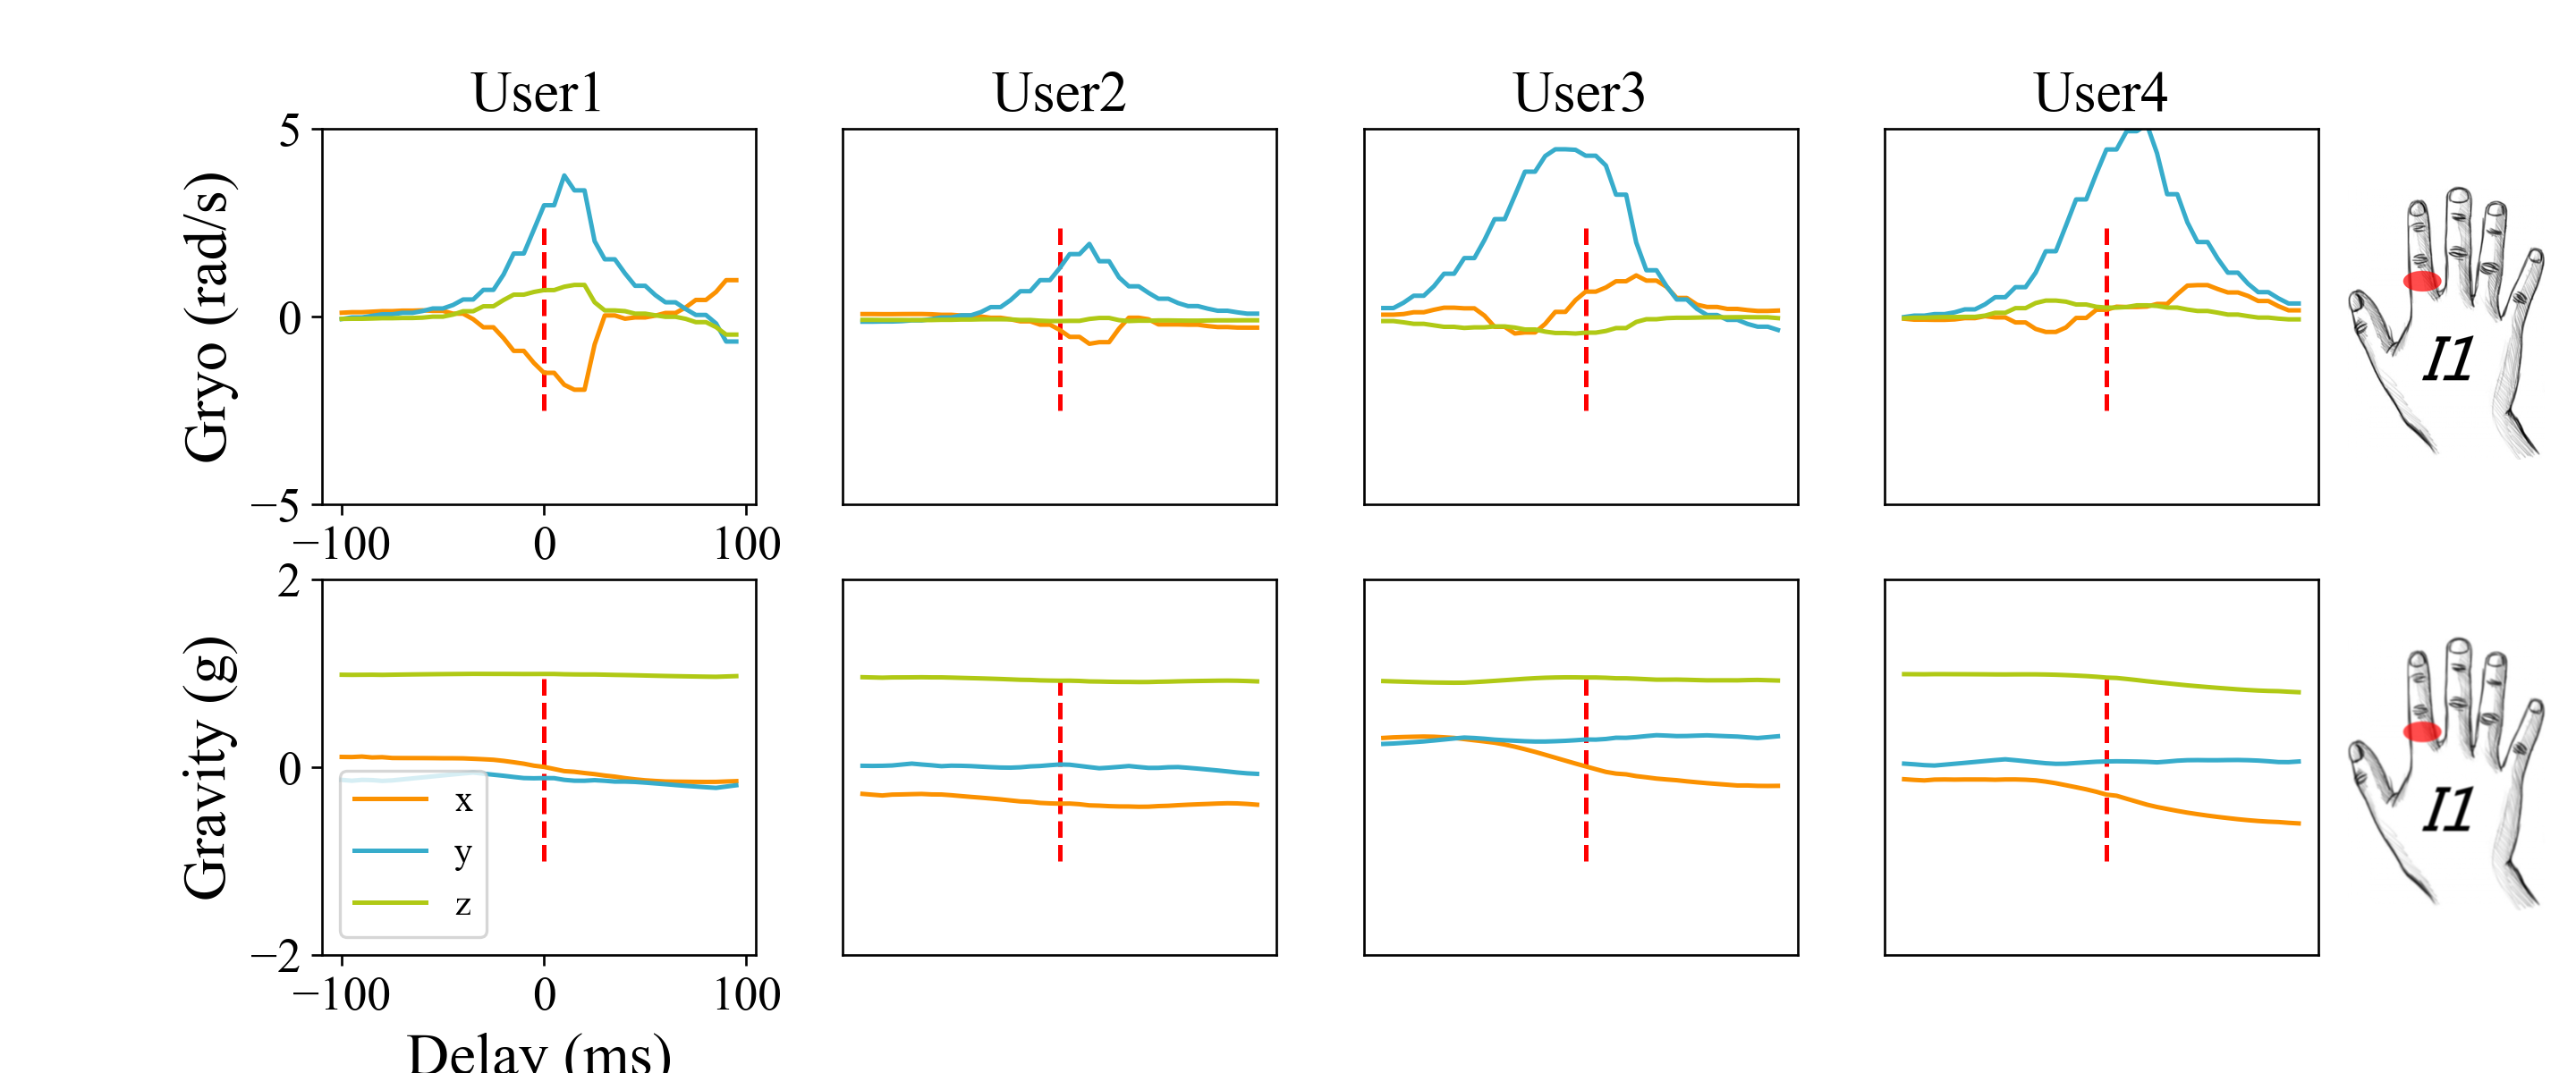
\includegraphics[width=0.8\linewidth]{IMU_gyr_hands.png}
	\caption*{图中展示了被试执行食指指腹触摸时惯性传感器的角速度和重力信号,其中惯性传感指环佩戴在食指第一指骨上,四纵列子图对应四个不同的被试。}
	\caption{角速度和重力信号图示}
	\label{fig:IMU_gyr_hands}
\end{figure}

如图\ref{fig:IMU_gyr_hands}所示是角速度和重力的波形。在触摸发生前后,角速度和重力变化也是有规律的,例如,由于触摸交互时人的手掌大致平行于交互表面,所以所有被试的重力数据都是相似的,若有一段手部运动的重力数据波形与图中所示的形态不符,说明它更有可能属于空中手势交互,而不是触摸交互。上述观察表明,来自惯性传感指环的可用信息是非常丰富的,若利用机器学习方法综合考虑各方面的有效信息,应能在触摸检测的性能上超越先前工作中的阈值方法\cite{lam2002mids, oh2017anywheretouch, niikura2014anywhere}。

\subsubsection{触摸检测分类器}

触摸检测分类器是根据一段时间内惯性传感信号,判断此刻是否发生触摸事件的二分类模型,是基于机器学习的触摸检测技术的核心。分类器从十帧(50毫秒)的传感信号中提取特征,对于九轴惯性传感器数据中的每一个维度,分类器计算其最大值、最小值、均值、偏度和峰度,然后将这些值拼接成45维的数组,作为机器学习模型的特征向量。

\begin{figure}
	\centering
	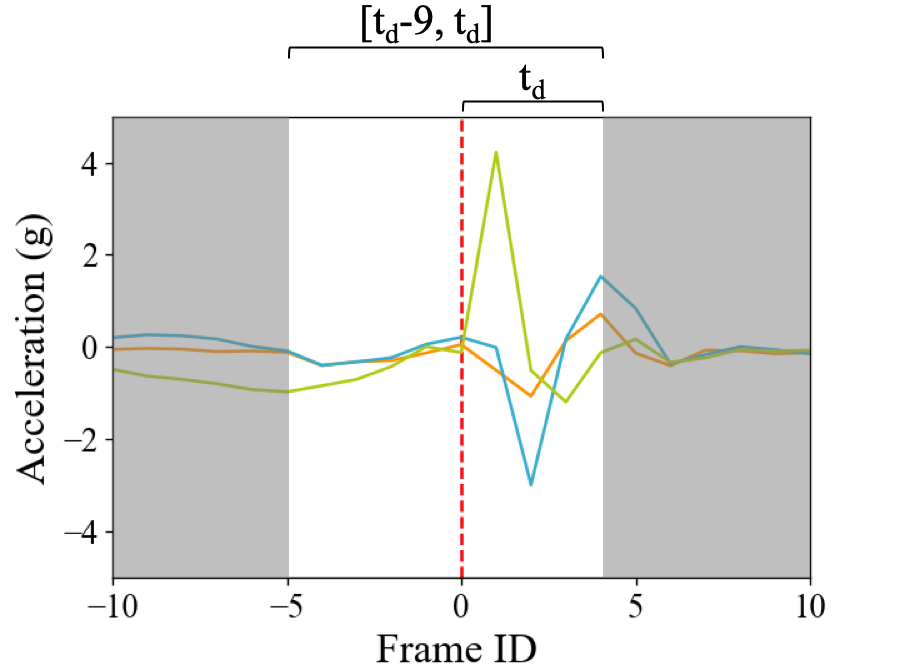
\includegraphics[width=0.8\linewidth]{tapping_ring_classifier.png}
	\caption*{触摸检测分类器是判断当前时刻是否发生触摸事件的二分类模型,其原理是将十帧(50毫秒)的传感信号提取成特征向量,而后使用支持向量机训练得模型。}
	\caption{触摸检测分类器}
	\label{fig:tapping_ring_classifier}
\end{figure}

如何选择信号采样的时间窗口,是一个值得探讨的问题。触摸导致的震动传输到惯性传感器的位置需要一定的时间,如果在震动抵达惯性传感器之前就贸然判定触摸事件是否发生,准确率会受到很大的影响。因此,在本小节所介绍的触摸检测技术中,检测延迟并不是越低越好,检测延迟和准确率是此消彼长的权衡惯性,实验者必须通过模拟实验来确定延迟的最佳取值。如图\ref{fig:tapping_ring_classifier}所示,本小节将$t_d(0<t_d<10)$定义为触摸检测分类器的延迟,设触摸发生在第0帧,则分类器由时间窗口$[t_d-9,t_d]$的信号所提取的特征训练而得。$t_d$的值的选取是一个值得权衡的问题,$t_d$的值越大,分类器就越能够利用触摸实际发生后的震动信号,分类的准确率将会提高,但与此同时检测的延迟也会增加。因此,实验者必须通过测试来给模型选定合适的延迟$t_d$。若给定$t_d$,分类器的训练过程如下:从时间窗口$[t_d-9,t_d]$的惯性传感信号中提取特征作为正样本;为了避免提前汇报触摸事件,需从时间窗口$[-14,-5]$的惯性传感信号中提取特征作为负样本;此外,需要从空中手势中截取信号,提取特征作为负样本。最后,针对以上正负样本数据集运行支持向量机来训练分类器模型。

\subsubsection{检测延迟优化}

上一小节提到,触摸检测分类器的检测延迟$t_d$是由技术实现者自行决定的,是一个检测准确率和延迟之间权衡的问题:一方面,检测延迟越低,触摸检测的准确率就越低;另一方面,检测延迟过高,又会直接影响用户体验。因此,如图\ref{fig:acc_over_delay}所示,实验者通过实验评测了$t_d$取不同的值时,触摸检测技术的准确率。从图中可以看出,总体上来说更高的检测延迟的确可以提高模型的预测准确率,但是当延迟提高至20毫秒以后,再往上延长检测时间的意义就不大了:混合方差分析表明,在20毫秒以内,模型的延迟$t_d$对模型预测准确率有显著性影响($F_{3,33}=133.4,p<.0001$);在20毫秒以后,图中的曲线就开始收敛了($F_{2,22}=0.011,p=.99$)。这说明,触摸检测分类器的检测延迟$t_d$应设置为20毫秒,既能支持较高的检测准确率(99.3\%),又能避免用户察觉到延迟的存在。

\begin{figure}
	\centering
	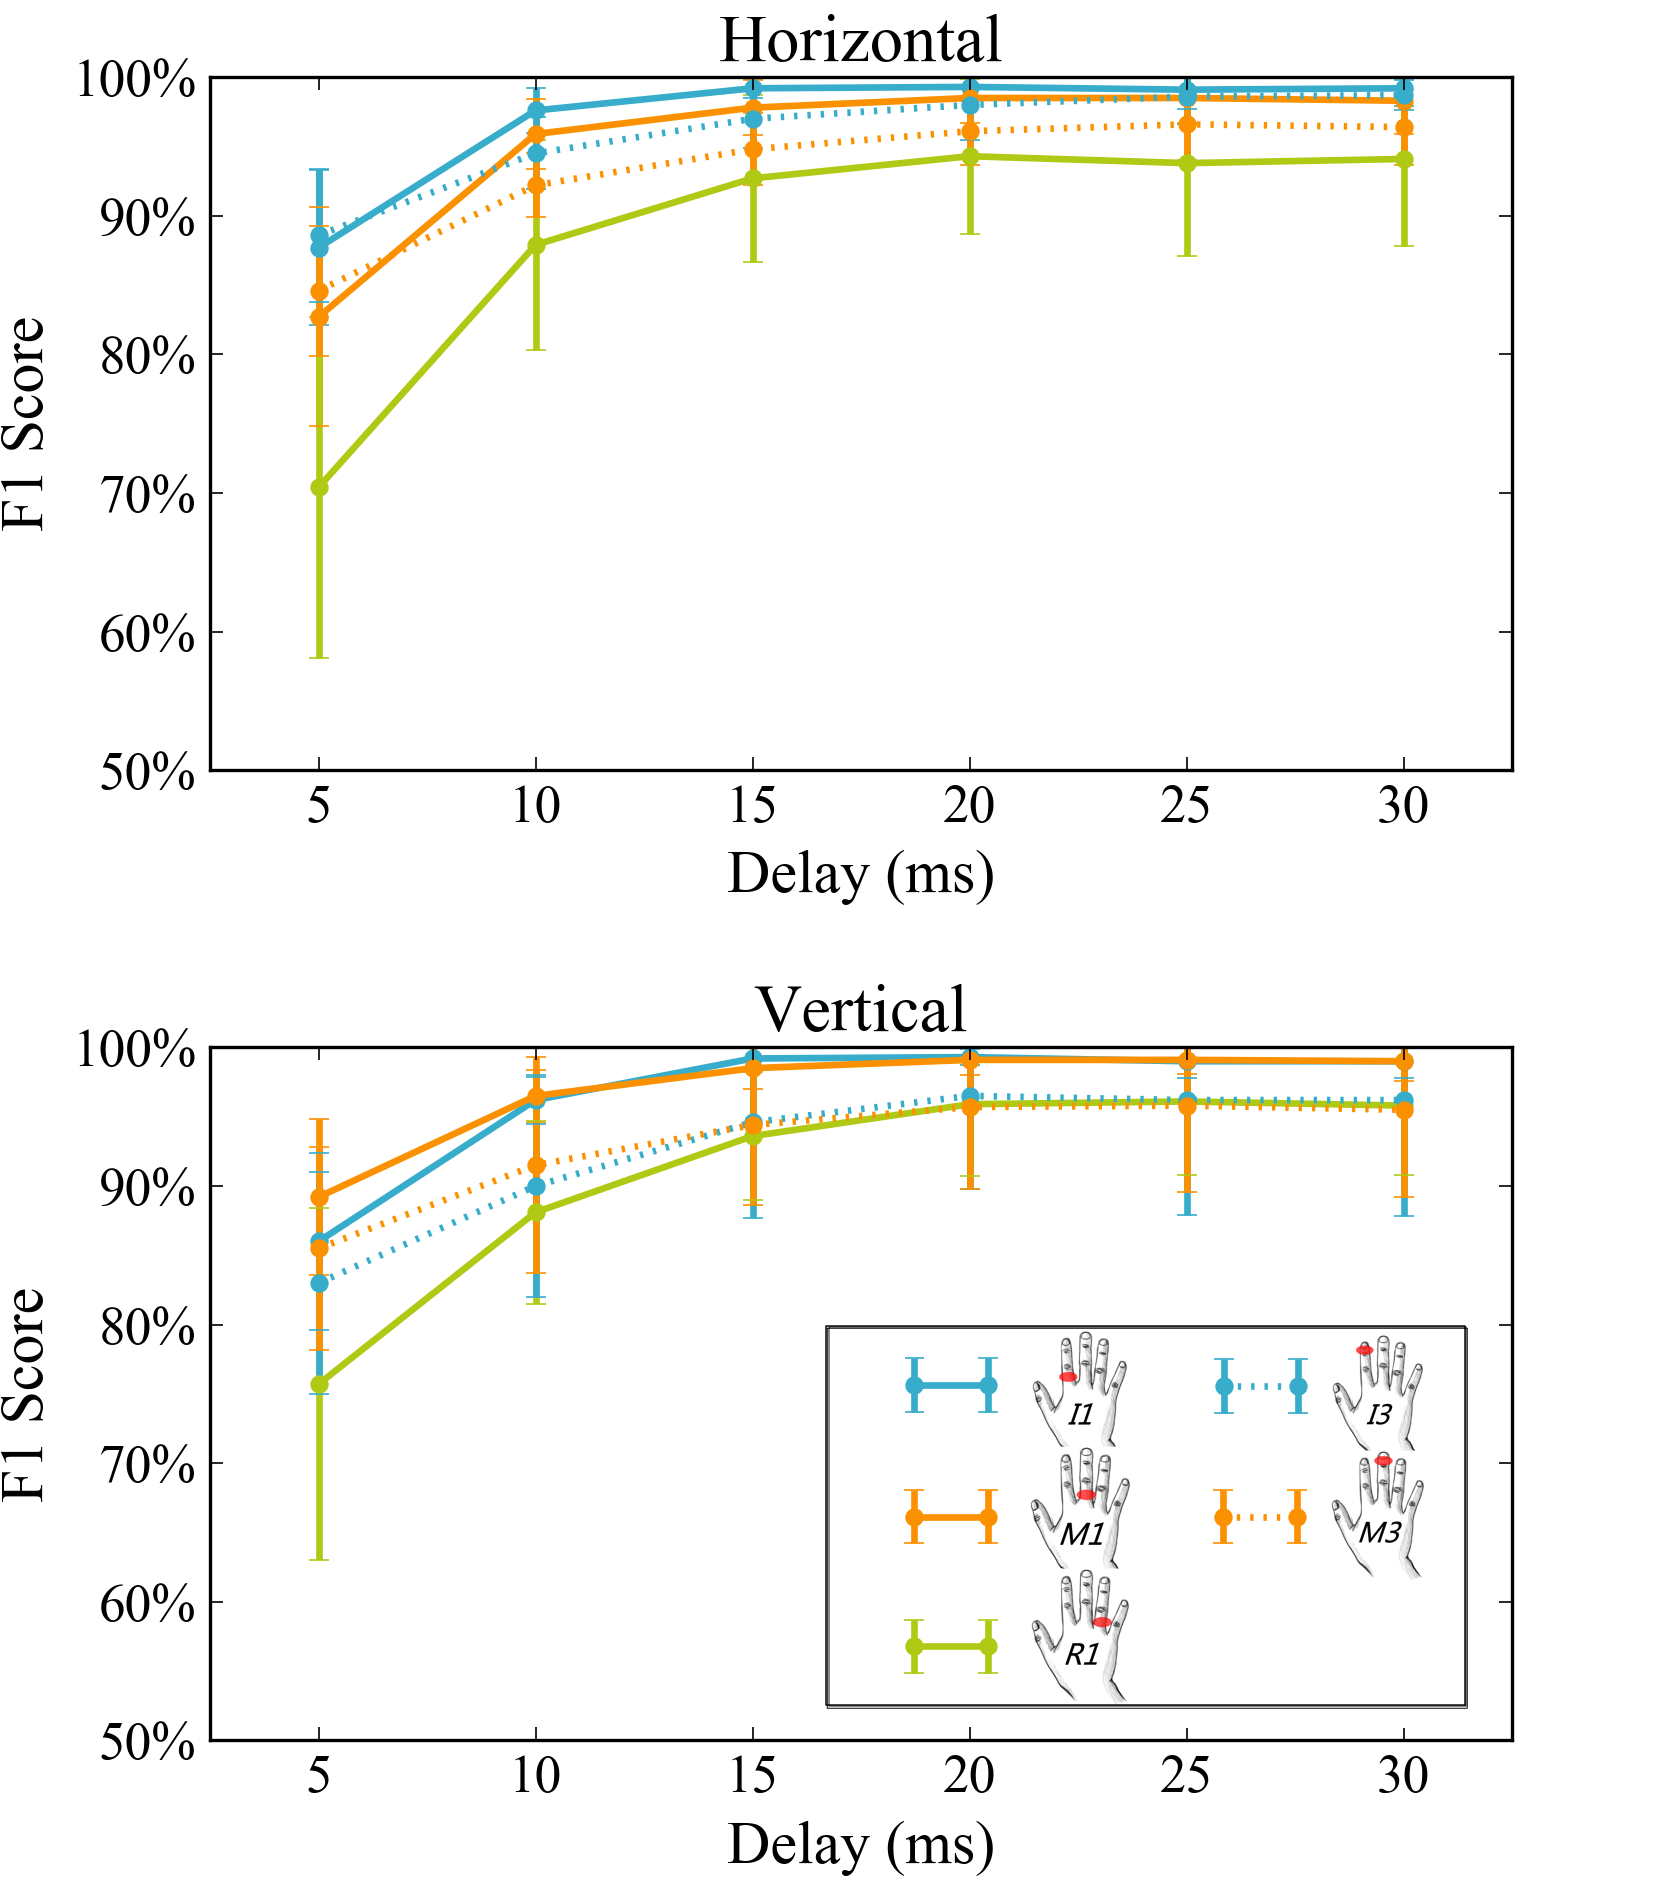
\includegraphics[width=0.8\linewidth]{acc_over_delay.png}
	\caption*{在本小节所介绍的触摸检测技术中,检测准确率和延迟之间是一个此消彼长的权衡问题,图中展示了指环佩戴在不同位置上时,检测准确率和延迟之间的关系。}
	\caption{触摸检测准确率与延迟之间的关系}
	\label{fig:acc_over_delay}
\end{figure}

\subsubsection{指环佩戴位置对比}

\begin{table}[!htbp]
	\centering
	\begin{tabular}{ll|l|l|l|l|l}
		\toprule
		& 指环位置 & I1               & M1            & R1            & I3             & M3            \\
		\midrule
		\multirow{3}{*}{水平} & 精准率 & 99.7\%(0.5\%) & 99.2\%(1.0\%) & 97.6\%(1.9\%) & 99.1\%(1.3\%)  & 98.3\%(1.4\%) \\
		& 召回率    & 98.9\%(1.6\%)    & 97.9\%(3.0\%) & 91.7\%(9.2\%) & 97.1\%(4.4\%)  & 94.1\%(4.1\%) \\
		& F1分数  & 99.3\%(1.0\%)    & 98.5\%(1.8\%) & 94.3\%(5.6\%) & 98.0\%(2.5\%)  & 96.1\%(2.5\%) \\ \hline
		\multirow{3}{*}{垂直}   & 精准率 & 99.7\%(0.6\%)    & 99.3\%(1.1\%) & 98.1\%(1.5\%) & 98.3\%(2.1\%)  & 98.4\%(1.9\%) \\
		& 召回率    & 99.0\%(0.9\%)    & 98.8\%(1.8\%) & 94.0\%(8.4\%) & 95.4\%(10.8\%) & 93.7\%(9.8\%) \\
		& F1分数  & 99.3\%(0.6\%)    & 99.1\%(1.1\%) & 95.9\%(5.3\%) & 96.5\%(6.7\%)  & 95.7\%(5.9\%) \\
		\bottomrule
	\end{tabular}
	\caption{指环佩戴在不同位置上时的触摸检测准确率(触摸检测延迟为20毫秒)}
	\label{tab:acc_over_placement}
\end{table}

在确定20毫秒的检测延迟效果最佳之后,实验者对比了20毫秒延迟下,指环佩戴在不同位置上的检测准确率。结果如表\ref{tab:acc_over_placement}所示,当指环佩戴在I1(食指第一指骨)上时,触摸检测分类器的性能是最好的,准确率(F1综合评价指标)达到99.3\%;次好的指环佩戴位置是M1(中指第一指骨),准确率为98.8\%。方差分析显示,指环佩戴位置对检测准确率有显著性影响($F_{4,44}=6.45,p<.001$),而交互表面的方向则对检测准确率没有显著影响($F_{1,11}=0.09,p=.76$)。后验检测显示I1指环佩戴位置显著优于R1(p<.001)、I3(p<.005)和M3(p<.005);M1显著优于R1(p<.005)、I3(p<.05)和M3(p<.01)。

实验一曾提到,实验者将指环佩戴位置I3和M3(食指、中指第三指骨)也加入了实验序列,其原因是实验者猜测此处能传感到更强的触摸震动,有利于触摸检测的准确率。然而,从本实验的结果看来,此猜测被证伪了,当指环佩戴在位置I3和M3上时触摸检测的准确率反而降低了。通过观察实验数据,实验者找到了两点原因:首先,虽然位置I3和M3上的惯性传感器能传感到更强的振动,但是其噪声也被放大了;其次,一根手指触摸交互表面所产生的震动不能很好地传递到另一根手指的指尖。

综合本小节实验结果和本章中对指环佩戴位置的主观喜好程度调研,将惯性传感指环佩戴在I1或M1位置(食指或中指第一指骨)上是最佳选择,既能提高指环触摸检测技术的检测准确率,又能满足用户的主观喜好。

\subsubsection{综合评测}

以上结果表明,触摸检测分类器在20毫秒的检测延迟下,在用户将惯性传感指环佩戴在食指第一指骨上时,性能最佳。因此,我们在此最佳设置下对触摸检测分类器做全面的评测。

\begin{figure}
	\centering
	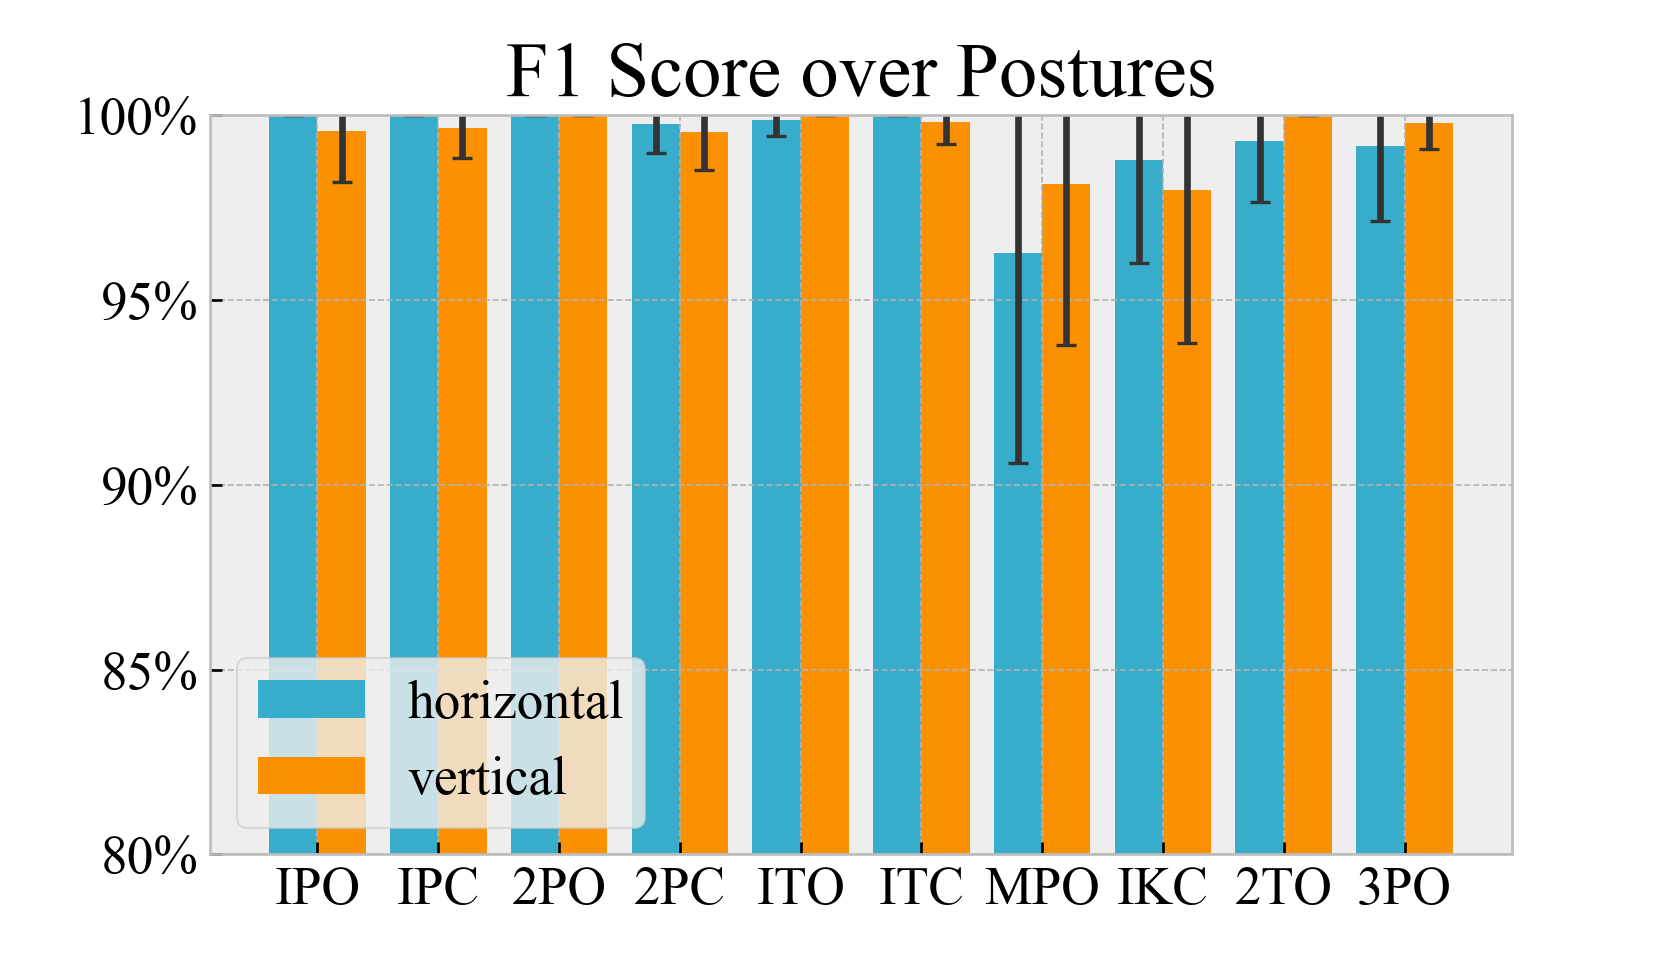
\includegraphics[width=0.8\linewidth]{acc_over_postures.png}
	\caption*{图中展示了触摸检测分类器对十种常用触摸姿态的触摸事件检测准确率,其中误差线表示标准差。}
	\caption{分类器对各触摸姿态的检测准确率}
	\label{fig:acc_over_postures}
\end{figure}

图\ref{fig:acc_over_postures}展示了不同触摸姿态下触摸检测的准确率(F1综合评价指标)。当被试执行敲击姿态MPO(中指指腹点击)和IKC(食指第二关节叩击)时,准确率超过95\%,其它触摸姿态的触摸事件检测准确率均接近100\%。这一结果说明,佩戴在食指上的惯性传感指环在感知食指触摸产生的震动时十分灵敏,而在感知其它手指触摸产生的震动时灵敏度有所下降,但其准确率仍然是可以接受的。

实验者设计了两种基线技术(baseline)用于与本小节所介绍的触摸检测技术做对比,这两种技术分别是基于震动和阈值的方法,和基于视觉的方法:(1)实验者仿照先前工作\cite{lam2002mids, oh2017anywheretouch}实现基于震动和阈值的触摸检测技术,并通过对本章所用数据集进行模拟实验来找到技术中所涉及参数的最优阈值;(2)实验者仿照先前工作\cite{newcombe2011kinectfusion, wilson2010combining, xiao2016direct, xiao2018mrtouch}实现了基于视觉方法的触摸检测技术,当摄像头检测到手指指尖与交互表面的距离下降到10毫米以下时,即汇报触摸事件。图\ref{fig:acc_vs_baseline}现实了本小节所介绍方法与两种基线技术之间的对比,方差分析表面本方法显著提高了触摸检测的精准率($F_{1,11}=10.4,p<.001$)和召回率($F_{1,11}=59.8,p<.0001$, $F_{1,11}=124.7,p<.0001$)。

\begin{figure}
	\centering
	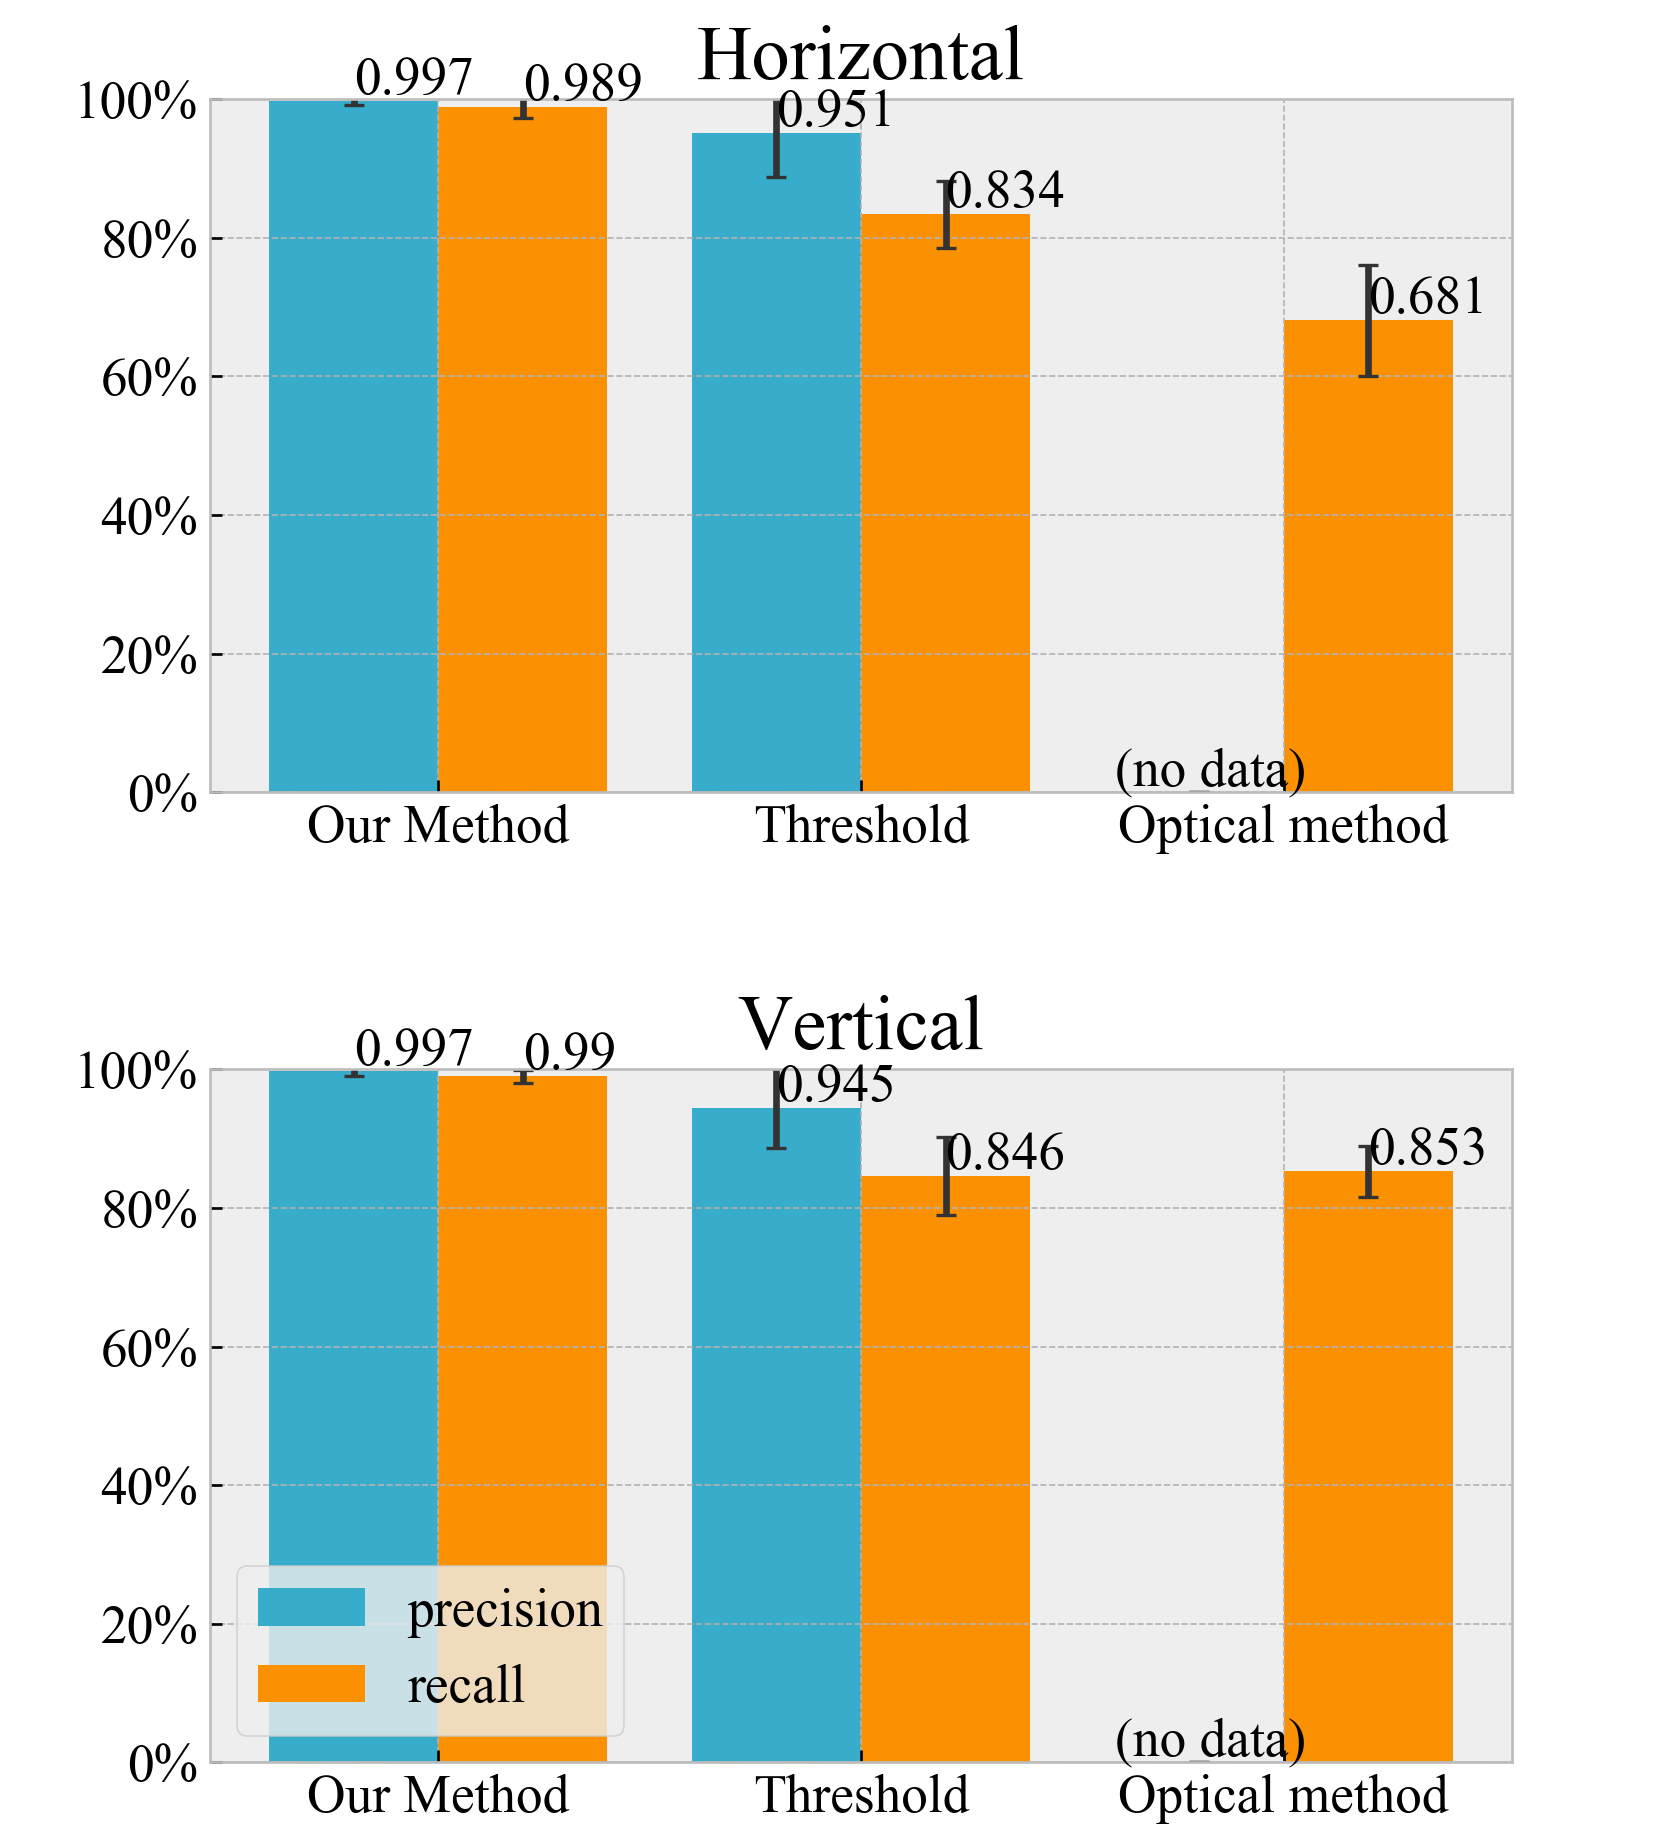
\includegraphics[width=0.8\linewidth]{acc_vs_baseline.png}
	\caption*{图中展示了本触摸检测技术在平均精准率和召回率上的对比,其中,误差线表示标准误差。实验中没有负样本可用于评测视觉方法的精准率。}
	\caption{本触摸检测技术与baseline的对比}
	\label{fig:acc_vs_baseline}
\end{figure}

\subsubsection{触摸检测算法流程}

触摸检测分类器只能就一段惯性传感信号,判断当前是否发生了触摸事件,然而,该分类器还不足以实时感知触摸,这是因为:(1)若时刻通过分类器判断触摸事件,分类器将在手指触摸交互表面后重复报告多次触摸事件;(2)虽然分类器的预测准确率高达99.3\%,但是传感器的运行频率为200赫兹,即每秒钟会调用200次分类器进行判断,这样一来误触的概率还是很大的。为了解决上述问题,实验者设计了一种基于触摸检测分类器的触摸检测算法:

\begin{itemize}
\item 如果在过去的十帧(50毫秒)内分类器预测过触摸事件,则算法不会重复报告触摸事件。
\item 只有当分类器连续两帧判定为触摸时,算法才会报告触摸事件。
\end{itemize}

上述算法会让检测延迟多一帧,但是,它能够大大降低误触的概率,并且不会重复报告多次触摸事件。本章将在实验三中通过实际的触摸交互任务评测该触摸检测算法的性能。

本小节介绍了基于支持向量机(SVM)的触摸检测技术,该方法只是简单版本的触摸检测技术,其目的在于探索清楚基于惯性传感指环的触摸交互技术中的诸多位置问题,为基于触摸运动模型的触摸交互技术打下基础。本小节所得出的结论如下所述:首先,先前工作中采用阈值方法判断触摸事件的方式是低效的,惯性传感指环能提供非常多有用的信息,用于支持低延迟的触摸检测技术;其次,将惯性传感指环佩戴在食指或中指的第一指骨上是最佳选择,该指环佩戴位置既符合用户的主观偏好,有能保证最高的触摸检测准确率;第三,触摸导致的震动能在10毫秒内传递到接触交互表面的手指上,能在20毫秒内传递到相邻手指上。其中,接触交互表面的手指的震感强烈,相邻手指第一指骨上的震感也强烈,但是相邻手指第三指骨处的震动已经不足以支撑高准确率的触摸检测了。上述结论为下一节内容,基于触摸运动模型的低延迟触摸检测技术奠定基础。

\section{基于触摸运动模型的触摸检测技术}

\subsection{基于触摸运动模型的触摸检测技术}\label{section:model_TappingRing}

基于触摸运动模型的触摸检测技术适用于运动传感信号,包括位移、速度和加速度信号。其中,基于摄像头的视觉方法可传感位移信号,惯性传感器可收集加速度信号。本章所提出的MR头盔加上惯性传感指环的智能设备系统可以获取触摸运动的位移和加速度信号,可用于支持低延迟触摸检测技术。本小节将分三种传感信道的情况讨论触摸运动模型如何指导触摸检测技术,这三种情况分别是:(1)仅有位移传感信号;(2)仅有加速度传感信号;(3)融合位移和加速度信号。

\textbf{(1)若仅有位移传感信号}:在追踪手指的过程中,设当前时刻的时间为$t_{now}$,用$t\in[t_{now}-60,t_{now}-10]$毫秒时间内的位移信号拟合无约束运动方程$x(\tau)=x_0+(x_1-x_0)(6\tau^5-15\tau^4+10\tau^3)$,使用信赖阈方法\cite{conn2000trust}进行拟合,若拟合成功,则说明此时手指正处于无约束运动过程中,需要观察手指是否停止运动,以判断手指是否接触到了交互表面。若当前位移测量值$x_m(\tau_{now})$与运动方程的预测值$x(\tau_{now})$相差超过传感信号的三倍标准误差时,可判定触摸事件发生:

\begin{equation}
	\lvert x_m(\tau_{now})-x(\tau_{now})\rvert>3\sigma_x
	\label{equ:touch_condition_x}
\end{equation}

若在成功拟合无约束运动方程后,始终不发上述公式所述情况,说明人的手指做出了空中点击的动作,而非真正的触摸点击。实验表明,触摸瞬间手指速度的经典值为$0.15m/s$,若位移传感信号的标准误差为0.5毫米,则根据上述公式,触摸事件的检测延迟为10毫秒左右。

\textbf{(2)若仅有加速度传感信号}:在记录手指加速度的过程中,设当前时刻的时间为$t_{now}$,用$t\in[t_{now}-60,t_{now}-10]$毫秒时间内的加速度信号拟合无约束运动的加速度方程$a(\tau)=(x_1-x_0)(120\tau^3-180\tau^2+60\tau)$,使用SLSQP算法进行拟合,若拟合成功,则说明此时手指正处于无约束运动过程中,需要观察手指运动是否达到一个很大的加速度,以判断手指是否接触到了交互表面。若当前加速度测量值$a_m(\tau_{now})$与运动方程的预测值$a(\tau_{now})$相差超过传感信号的三倍标准误差时,可判定触摸事件发生:

\begin{equation}
	\lvert a_m(\tau_{now})-a(\tau_{now})\rvert>3\sigma_a
	\label{equ:touch_condition_a}
\end{equation}

由于触摸运动的位移方程在触摸瞬间$t=t_c$不可导,公式揭示此时的加速度无限大。但实际上,手指不是理想的刚体,所以加速度不可能是无限大,而仅仅是相当大。若惯性传感器紧贴在食指的第一关节骨上,它的加速度会在碰撞发生后的10毫秒内达峰值,触摸事件的检测延迟应为10毫秒左右。

\textbf{(3)融合位移和加速度传感信号}:

若同时有位移信号和加速度信号,可以融合两种信号,在保持准确率不变的情况下降低触摸事件检测的延迟。在当前时刻$t_{now}$,位移信号服从正态分布$N(x(\tau_{now}),\sigma_x)$,设位移信号的概率密度函数为$f_x(x_m(\tau_{now}))$:

\begin{equation}
	f_x(x_m(\tau_{now}))=\frac{1}{\sqrt{2\pi}\sigma_x}exp\left(-\frac{(x_m(\tau_{now})-x(\tau_{now}))^2}{2\sigma_x}\right)
\end{equation}

同理,设加速度信号误差的概率密度函数为$f_a(a_m(\tau_{now}))$,则公式\ref{equ:touch_condition_x}、公式\ref{equ:touch_condition_a}分别对应:

\begin{equation}
	\int_{\lvert x_m(\tau_{now})-x(\tau_{now})\rvert<3\sigma_x}f_x(x_m(\tau_{now}))>99.7\%
\end{equation}

\begin{equation}
	\int_{\lvert a_m(\tau_{now})-a(\tau_{now})\rvert<3\sigma_x}f_a(a_m(\tau_{now}))>99.7\%
\end{equation}

由于卡尔曼滤波已经有效利用位移信号和加速度信号的互信息,降低了两者的标准误差,此时可认为位移的误差与加速度的误差相互独立,因此下述公式成立时可判定触摸事件发生:

\begin{equation}
	\int_{\frac{\lvert x_m(\tau_{now})-x(\tau_{now})\rvert^2}{(3\sigma_x)^2}+\frac{\lvert a_m(\tau_{now})-a(\tau_{now})\rvert^2}{(3\sigma_a)^2}<1}f_x(x_m(\tau_{now}))f_a(a_m(\tau_{now}))>99.7\%
\end{equation}

简化以上公式得到,当下述公式成立时可判定触摸事件发生:

\begin{equation}
	\frac{\lvert x_m(\tau_{now})-x(\tau_{now})\rvert^2}{(3\sigma_x)^2}+
	\frac{\lvert a_m(\tau_{now})-a(\tau_{now})\rvert^2}{(3\sigma_a)^2}>1
\label{equ:x_a_judgement}
\end{equation}

以上就是触摸运动模型对触摸检测技术的计算理论指导,根据上述数学推导,接下来将介绍触摸检测的算法流程:

\begin{enumerate}
\item 通过摄像头和视觉的方法实时采集用户手指的位移信号,通过佩戴在手指上的惯性传感指环采集手指的加速度信号,每一时刻都截取从当前时刻往前推100毫秒内的信号数据,作后续处理。
\item 根据Madgwick算法\cite{madgwick2010efficient}计算指环加速度信号在重力方向上的投影,然后根据第二章所介绍的触摸运动模型的计算方法,拟合当前的无约束运动方程,若拟合成功,则说明此时手指正处于无约束运动过程中,跳至下一步骤。
\item 开始检测手指的位移和加速度信号是否满足公式\ref{equ:x_a_judgement},若满足,则判定触摸事件已发生,若在无约束运动方程拟合成功后20毫秒内,公式\ref{equ:x_a_judgement}未得到满足,则回到上一步骤
\end{enumerate}

以上就是基于触摸运动模型的触摸检测算法,接下来一节将通过真实的触摸交互任务评测本技术,同时对比本小节中提到的一系列初探的或先前工作的触摸检测技术。

\subsection{实验三:评测本节触摸检测技术}

本实验通过实际的触摸交互应用程序评测本章所提出的触摸检测技术,实验共对比了三种不同的触摸检测技术,分别是:(1)基线(baseline)技术,先前工作中基于视觉的触摸检测技术\cite{xiao2018mrtouch};(2)本章第3.7节中介绍的,基于机器学习的触摸检测技术;(3)本章第3.8节中介绍的,基于触摸运动模型的低延迟触摸检测技术。为了让上述技术在尽可能苛刻的条件下接受评测,实验者选取了一款名为“别碰白键”的游戏作为实验的交互任务,该游戏要求玩家进行尽可能快速的连续触摸点击。

\subsubsection{实验设计和过程}

实验者从校园中招募了12名被试,其中3名为女性,被试的年龄从20岁到28岁不等,平均年龄为23.2岁。这一批被试未参与之前的任何一个用户实验。实验共分为两大部分,被试分别在水平的桌面和垂直的墙面上进行游戏。每一部分的实验又包含三段实验,每段实验采用不同的触摸检测技术。采取组内实验设计,即每一名被试都要使用不同的触摸检测技术进行实验,为了避免学习效应,实验者采用拉丁方来平衡不同触摸检测技术的实验顺序。

实验中,被试像实验二那样佩戴惯性传感指环,同时,在头上佩戴手型追踪摄像头LeapMotion,实验设置图同实验二的\ref{fig:tapping_ring_config}。被试将指环佩戴在食指第一关节上,通过最常用的触摸姿态,即食指指腹点击进行触摸交互。如图\ref{fig:tapping_ring_app}所示,本实验在一个显示器上展示了“别碰白键”这款游戏,同时也在游戏中渲染了被试的虚拟手,显控比为1:1。“别碰白键”这款游戏的目标是尽可能快速地通过触摸来点击从屏幕顶部出现的黑色按键,同时避开白色按键。每点中一个黑色按键,新一行的按键就会从屏幕的顶部弹出;如果被试不慎点中了白色按键,屏幕就会闪烁一秒以报告错误。游戏中,被试需要点击100个黑色按键来结束游戏,游戏的目标是尽快点击完这100个黑色按键。

\begin{figure}
	\centering
	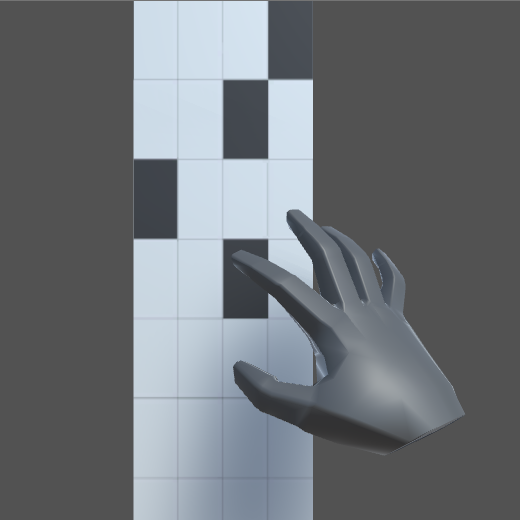
\includegraphics[width=0.6\linewidth]{tapping_ring_app.png}
	\caption*{图中所示为本实验的交互任务:别碰白键,这是一款要求用户以尽可能快的速度进行连续触摸的游戏,能够有效测试触摸检测技术的性能。}
	\caption{实验任务图示}
	\label{fig:tapping_ring_app}
\end{figure}

本实验的总时长为20分钟,我们通过触摸检测的准确率、延迟,和用户完成任务的时间来评价三种不同触摸测试技术的性能。

\subsubsection{实验结果}

\begin{table}[!htbp]
	\centering
	\begin{tabular}{l|lll}
		\toprule
		& 基于视觉方法\cite{xiao2018mrtouch}  & 基于机器学习 & 基于触摸运动模型 \\
		\midrule
		精准率 & 85.42\%(10.42\%) & 98.62\%(2.50\%) & 99.32(0.74\%) \\
		召回率 & 84.08\%(9.24\%) & 98.61\%(1.33\%)  & 99.17(0.88\%) \\
		任务完成时间(秒) & 44.30(19.19) & 35.74(13.69) & 36.21(14.82) \\
		检测延迟(毫秒) & 5.48(15.07) & 9.11(3.41) & 9.02(3.16) \\
		\bottomrule
	\end{tabular}
	\caption{表格对比了不同触摸检测技术的性能,括号中的数值为标准差。}
	\label{tab:tapping_ring_study3}
\end{table}

%请注意,表中的延迟是所评测技术的延迟和低延迟触摸板测量值(本实验的真值)之间的差距。因此实际延迟还可能多0到5毫秒,来至低延迟触摸板的延迟。

表\ref{tab:tapping_ring_study3}展示了实验的评测结果。在检测准确率(F1综合评价指标)方面,方差分析表明,无论是基于触摸运动模型的触摸检测技术($F_{1,11}=87.9,p<.001$),还是基于机器学习的方法($F_{1,11}=53.6,p<.001$),都显著优于先前工作中基于视觉的方法。通过分析视觉方法中的错误案例能发现,本实验的交互任务要求被试连续快速触摸,基于视觉的方法不能很好的处理这种情况,例如,基于视觉的方法认为手指离开交互表面超过15毫米才算一次触摸动作完成,但在连续快速触摸任务中,连续两次触摸之间被试的手指可能从未离开交互表面超过15毫米,这影响了第二次触摸事件的检测。而在本章所提出的两种触摸检测技术的比较中,基于触摸运动模型的触摸检测技术的准确率超过99\%,显著高于基于机器学习方法的准确率($F_{1,11}=5.6,p<.05$)。数据分析发现,这一差异主要来源于对较轻的触摸的检测,基于触摸运动模型的触摸检测技术检测更准确,这可能是因为基于模型的方法更好地利用了触摸之前手指向下运动的信息。

在被试完成实验任务的时间方面,方差分析表明,基于触摸运动模型的触摸检测技术($F_{1,11}=7.9,p<.05$)和基于机器学习的方法($F_{1,11}=8.3,p<.05$),都显著优于先前工作中基于视觉的方法。这是因为在视觉方法中,过高的检测错误率让被试经常需要纠正错误,延误了完成任务的时间。而在本章所提出的两种触摸检测技术的比较中,被试完成任务的时间没有显著性差异。

在检测延迟这方面,基于机器学习或触摸运动模型的触摸检测技术的延迟都稳定在10毫秒以内。而基于视觉的方法的检测延迟则非常不稳定,从表格中可以看到,视觉方法的检测延迟平均值为5.48毫秒,但是其标准差却高达15.07毫秒。有的时候视觉方法甚至会提前汇报触摸事件,导致负延迟的情况,这是因为视觉方法规定,当手指与交互表面下降到10毫米阈值以下时,即报告触摸事件。采访被试发现,没有被试能在基于机器学习或触摸运动模型的触摸检测技术下察觉到延迟的存在,但在基于视觉方法的技术中,则能明显感受到延迟忽快忽慢。

综合上述实验结果,基于触摸运动模型的触摸检测技术具有很高的检测准确率,显著高于先前工作,也显著高于基于简单机器学习的方法。而在检测延迟这方面,基于触摸运动模型的触摸检测技术也显著优于先前工作。这说明,基于惯性传感指环的触摸检测技术很具有实用前景,值得更多的关注。

\section{本章小结}

任意无源表面上的触摸交互很可能是未来的一种主要人机交互方式,头戴式混合现实系统可以在普通物体表面上叠加交互界面,使得这些物体表面上的触摸交互成为可能。先前工作已经提出利用MR头盔的前置摄像头跟踪手型\cite{xiao2018mrtouch},但是相关工作在判断手指是否接触到交互表面上时遇到了困难。本章内容是第一份专注于优化惯性传感指环触摸检测技术的研究。评测结果表明,基于触摸运动模型的指环触摸检测技术可以在10毫秒以内的低延迟下检测触摸事件,召回率高达99.17\%,误触率仅为0.68\%。低延迟是本触摸交互技术的核心贡献之一,这是因为,人在触摸交互中无法察觉到低于24毫秒的延迟\cite{jota2013fast},而本技术的延迟仅为10毫秒,在响应性上提供了最佳的用户体验。从原理的角度来看,基于触摸运动模型的触摸检测技术性能更优有其底层逻辑:(1)触摸运动模型充分利用了多帧信息,降低单帧信号误差带来的影响;(2)无需直接观测触摸点,有效回避视觉遮挡问题\cite{xiao2018mrtouch}。

% !TeX root = ../thuthesis-example.tex

\chapter{面向连续触摸输入的防误触技术}



% 其他部分
\backmatter

% 参考文献
\bibliography{ref/refs}  % 参考文献使用 BibTeX 编译
% \printbibliography       % 参考文献使用 BibLaTeX 编译

% 附录
\appendix
% % !TeX root = ../thuthesis-example.tex

\begin{survey}
\label{cha:survey}

\title{Title of the Survey}
\maketitle


\tableofcontents


本科生的外文资料调研阅读报告。


\section{Figures and Tables}

\subsection{Figures}

An example figure in appendix (Figure~\ref{fig:appendix-survey-figure}).

\begin{figure}
  \centering
  
\includegraphics[width=0.6\linewidth]{example-image-a.pdf}
  \caption{Example figure in appendix}
  \label{fig:appendix-survey-figure}
\end{figure}


\subsection{Tables}

An example table in appendix (Table~\ref{tab:appendix-survey-table}).

\begin{table}
  \centering
  \caption{Example table in appendix}
  \begin{tabular}{ll}
    \toprule
    File name       & Description                                         \\
    \midrule
    thuthesis.dtx   & The source file including documentaion and comments \\
    thuthesis.cls   & The template file                                   \\
    thuthesis-*.bst & BibTeX styles                                       \\
    thuthesis-*.bbx & BibLaTeX styles for bibliographies                  \\
    thuthesis-*.cbx & BibLaTeX styles for citations                       \\
    \bottomrule
  \end{tabular}
  \label{tab:appendix-survey-table}
\end{table}


\section{Equations}

An example equation in appendix (Equation~\eqref{eq:appendix-survey-equation}).
\begin{equation}
  \frac{1}{2 \uppi \symup{i}} \int_\gamma f = \sum_{k=1}^m n(\gamma; a_k) \mathscr{R}(f; a_k)
  \label{eq:appendix-survey-equation}
\end{equation}


\section{Citations}

Example citations in appendix.
\cite{abrahams99tex}
\cite{salomon1995advanced}
\cite{abrahams99tex,salomon1995advanced}


\bibliographystyle{unsrtnat}
\bibliography{ref/appendix}

\end{survey}
       % 本科生:外文资料的调研阅读报告
% % !TeX root = ../thuthesis-example.tex

\begin{translation}
\label{cha:translation}

\title{书面翻译题目}
\maketitle

\tableofcontents


本科生的外文资料书面翻译。


\section{图表示例}

\subsection{图}

附录中的图片示例(图~\ref{fig:appendix-translation-figure})。

\begin{figure}
  \centering
  
\includegraphics[width=0.6\linewidth]{example-image-a.pdf}
  \caption{附录中的图片示例}
  \label{fig:appendix-translation-figure}
\end{figure}


\subsection{表格}

附录中的表格示例(表~\ref{tab:appendix-translation-table})。

\begin{table}
  \centering
  \caption{附录中的表格示例}
  \begin{tabular}{ll}
    \toprule
    文件名          & 描述                         \\
    \midrule
    thuthesis.dtx   & 模板的源文件,包括文档和注释 \\
    thuthesis.cls   & 模板文件                     \\
    thuthesis-*.bst & BibTeX 参考文献表样式文件    \\
    thuthesis-*.bbx & BibLaTeX 参考文献表样式文件  \\
    thuthesis-*.cbx & BibLaTeX 引用样式文件        \\
    \bottomrule
  \end{tabular}
  \label{tab:appendix-translation-table}
\end{table}


\section{数学公式}

附录中的数学公式示例(公式\eqref{eq:appendix-translation-equation})。
\begin{equation}
  \frac{1}{2 \uppi \symup{i}} \int_\gamma f = \sum_{k=1}^m n(\gamma; a_k) \mathscr{R}(f; a_k)
  \label{eq:appendix-translation-equation}
\end{equation}


\section{文献引用}

文献引用示例\cite{abrahams99tex}。


% 书面翻译的参考文献
\bibliographystyle{unsrtnat}
\bibliography{ref/appendix}

% 书面翻译对应的原文索引
\begin{translation-index}
  \nocite{salomon1995advanced}
  \bibliographystyle{unsrtnat}
  \bibliography{ref/appendix}
\end{translation-index}

\end{translation}
  % 本科生:外文资料的书面翻译
% !TeX root = ../thuthesis-example.tex

\chapter{补充内容}

附录是与论文内容密切相关、但编入正文又影响整篇论文编排的条理和逻辑性的资料,例如某些重要的数据表格、计算程序、统计表等,是论文主体的补充内容,可根据需要设置。


\section{图表示例}

\subsection{图}

附录中的图片示例(图~\ref{fig:appendix-figure})。

\begin{figure}
  \centering
  
\includegraphics[width=0.6\linewidth]{example-image-a.pdf}
  \caption{附录中的图片示例}
  \label{fig:appendix-figure}
\end{figure}


\subsection{表格}

附录中的表格示例(表~\ref{tab:appendix-table})。

\begin{table}
  \centering
  \caption{附录中的表格示例}
  \begin{tabular}{ll}
    \toprule
    文件名          & 描述                         \\
    \midrule
    thuthesis.dtx   & 模板的源文件,包括文档和注释 \\
    thuthesis.cls   & 模板文件                     \\
    thuthesis-*.bst & BibTeX 参考文献表样式文件    \\
    thuthesis-*.bbx & BibLaTeX 参考文献表样式文件  \\
    thuthesis-*.cbx & BibLaTeX 引用样式文件        \\
    \bottomrule
  \end{tabular}
  \label{tab:appendix-table}
\end{table}


\section{数学公式}

附录中的数学公式示例(公式\eqref{eq:appendix-equation})。
\begin{equation}
  \frac{1}{2 \uppi \symup{i}} \int_\gamma f = \sum_{k=1}^m n(\gamma; a_k) \mathscr{R}(f; a_k)
  \label{eq:appendix-equation}
\end{equation}


% 致谢
% !TeX root = ../thuthesis-example.tex

\begin{acknowledgements}
  衷心感谢导师×××教授和物理系××副教授对本人的精心指导。他们的言传身教将使我终生受益。

  在美国麻省理工学院化学系进行九个月的合作研究期间,承蒙 Robert Field 教授热心指导与帮助,不胜感激。

  感谢×××××实验室主任×××教授,以及实验室全体老师和同窗们学的热情帮助和支持!

  本课题承蒙国家自然科学基金资助,特此致谢。
\end{acknowledgements}


% 声明
\statement
% 将签字扫描后的声明文件 scan-statement.pdf 替换原始页面
% \statement[file=scan-statement.pdf]
% 本科生编译生成的声明页默认不加页脚,插入扫描版时再补上;
% 研究生编译生成时有页眉页脚,插入扫描版时不再重复。
% 也可以手动控制是否加页眉页脚
% \statement[page-style=empty]
% \statement[file=scan-statement.pdf, page-style=plain]

% 个人简历、在学期间完成的相关学术成果
% !TeX root = ../thuthesis-example.tex

\begin{resume}

  \section*{个人简历}

1995年5月12日出生于广东省中山市

2013年9月考入清华大学计算机系计算机专业,2017年7月本科毕业并获得学士学位。

2017年9月保研进入清华大学计算机系攻读人机交互专业博士至今。

 \section*{在学期间完成的相关学术成果}

 \subsection*{学术论文}

第一作者发表论文

\begin{achievements}
 	\item \textbf{Gu Y}, Yu C, Chen X, et al. Typeboard: Identifying unintentional touch on pressure-sensitive touchscreen keyboards[C]//The 34th Annual ACM Symposium on User Interface Software and Technology. 2021: 568-581. (TH-CPL Rank A)
 	\item \textbf{Gu Y}, Yu C, Li Z, et al. Qwertyring: Text entry on physical surfaces using a ring[J]. Proceedings of the ACM on Interactive, Mobile, Wearable and Ubiquitous Technologies, 2020, 4(4): 1-29. (TH-CPL Rank A)
 	\item \textbf{Gu Y}, Yu C, Li Z, et al. Accurate and low-latency sensing of touch contact on any surface with finger-worn imu sensor[C]//Proceedings of the 32nd Annual ACM Symposium on User Interface Software and Technology. 2019: 1059-1070. (TH-CPL Rank A)

\end{achievements}

共同一作发表论文

\begin{achievements}
	\item Liu G, \textbf{Gu Y}, Yin Y, et al. Keep the phone in your pocket: Enabling smartphone operation with an imu ring for visually impaired people[J]. Proceedings of the ACM on Interactive, Mobile, Wearable and Ubiquitous Technologies, 2020, 4(2): 1-23. (TH-CPL Rank A)
\end{achievements}

学生一作发表论文

\begin{achievements}
	\item Yu C, \textbf{Gu Y}, Yang Z, et al. Tap, dwell or gesture? exploring head-based text entry techniques for hmds[C]//Proceedings of the 2017 CHI Conference on Human Factors in Computing Systems. 2017: 4479-4488. (TH-CPL Rank A)
\end{achievements}

非第一作者发表论文

\begin{achievements}
	\item Yu C, Wei X, Vachher S, Qin Y, Liang C, Weng Y, \textbf{Gu Y}, et al. Handsee: enabling full hand interaction on smartphone with front camera-based stereo vision[C]//Proceedings of the 2019 CHI Conference on Human Factors in Computing Systems. 2019: 1-13. (TH-CPL Rank A)
\end{achievements}

\subsection*{专利}

\begin{achievements}
\item 史元春, 喻纯, \textbf{古裔正}. 2021.07. 一种抬起手势的识别方法、系统、电子设备及存储介质. CN111580664A. (中国专利申请号,已授权)
\item 史元春, 喻纯, 秦岳, \textbf{古裔正}, 韦笑颖. 2021.07. 智能电子设备上基于单摄像头的双目视觉与物体识别技术. CN109993059B. (中国专利申请号,已授权)
\item 喻纯, \textbf{古裔正}, 杨志灿, 阎裕康, 史元春. 2018.08. 手型跟踪装置. CN207752443U. (实用新型,已授权)
\item 史元春, 喻纯, \textbf{古裔正}, 周诚驰, 张磊. 2022.01. 一种二维码扫描方法、装置及电子设备. CN113935348A.(中国专利公开号,已公开)
\item 史元春, 喻纯, \textbf{古裔正}, 周诚驰, 张磊. 2022.01. 一种控制智能家电的方法、装置及电子设备. CN113934150A.(中国专利公开号,已公开)
\item 史元春, 喻纯, \textbf{古裔正}. 2021.11. 触摸屏防误触的方法及装置、电子设备及存储介质. CN113608634A. (中国专利公开号,已公开)
\item 史元春, 喻纯, \textbf{古裔正}. 2020.08. 一种信息输入方法、系统、电子设备及存储介质. CN111580663A. (中国专利公开号,已公开)
\item 史元春, 喻纯, 刘冠宏, \textbf{古裔正}.2020.08. 一种设备控制方法、电子设备、设备控制系统及存储介质. CN111580666A.(中国专利公开号,已公开)
\end{achievements}

\end{resume}


% 指导教师/指导小组学术评语
% !TeX root = ../thuthesis-example.tex

\begin{comments}
% \begin{comments}[name = {指导小组学术评语}]
% \begin{comments}[name = {Comments from Thesis Supervisor}]
% \begin{comments}[name = {Comments from Thesis Supervision Committee}]

  论文提出了……

\end{comments}


% 答辩委员会决议书
% !TeX root = ../thuthesis-example.tex

\begin{resolution}

  论文提出了……

  论文取得的主要创新性成果包括:

  1. ……

  2. ……

  3. ……

  论文工作表明作者在×××××具有×××××知识,具有××××能力,论文××××,答辩××××。

  答辩委员会表决,(×票/一致)同意通过论文答辩,并建议授予×××(姓名)×××(门类)学博士/硕士学位。

\end{resolution}


% 本科生的综合论文训练记录表(扫描版)
% \record{file=scan-record.pdf}

\end{document}
